% Options for packages loaded elsewhere
\PassOptionsToPackage{unicode}{hyperref}
\PassOptionsToPackage{hyphens}{url}
%
\documentclass[
]{book}
\usepackage{amsmath,amssymb}
\usepackage{lmodern}
\usepackage{iftex}
\ifPDFTeX
  \usepackage[T1]{fontenc}
  \usepackage[utf8]{inputenc}
  \usepackage{textcomp} % provide euro and other symbols
\else % if luatex or xetex
  \usepackage{unicode-math}
  \defaultfontfeatures{Scale=MatchLowercase}
  \defaultfontfeatures[\rmfamily]{Ligatures=TeX,Scale=1}
\fi
% Use upquote if available, for straight quotes in verbatim environments
\IfFileExists{upquote.sty}{\usepackage{upquote}}{}
\IfFileExists{microtype.sty}{% use microtype if available
  \usepackage[]{microtype}
  \UseMicrotypeSet[protrusion]{basicmath} % disable protrusion for tt fonts
}{}
\makeatletter
\@ifundefined{KOMAClassName}{% if non-KOMA class
  \IfFileExists{parskip.sty}{%
    \usepackage{parskip}
  }{% else
    \setlength{\parindent}{0pt}
    \setlength{\parskip}{6pt plus 2pt minus 1pt}}
}{% if KOMA class
  \KOMAoptions{parskip=half}}
\makeatother
\usepackage{xcolor}
\usepackage{color}
\usepackage{fancyvrb}
\newcommand{\VerbBar}{|}
\newcommand{\VERB}{\Verb[commandchars=\\\{\}]}
\DefineVerbatimEnvironment{Highlighting}{Verbatim}{commandchars=\\\{\}}
% Add ',fontsize=\small' for more characters per line
\usepackage{framed}
\definecolor{shadecolor}{RGB}{248,248,248}
\newenvironment{Shaded}{\begin{snugshade}}{\end{snugshade}}
\newcommand{\AlertTok}[1]{\textcolor[rgb]{0.94,0.16,0.16}{#1}}
\newcommand{\AnnotationTok}[1]{\textcolor[rgb]{0.56,0.35,0.01}{\textbf{\textit{#1}}}}
\newcommand{\AttributeTok}[1]{\textcolor[rgb]{0.77,0.63,0.00}{#1}}
\newcommand{\BaseNTok}[1]{\textcolor[rgb]{0.00,0.00,0.81}{#1}}
\newcommand{\BuiltInTok}[1]{#1}
\newcommand{\CharTok}[1]{\textcolor[rgb]{0.31,0.60,0.02}{#1}}
\newcommand{\CommentTok}[1]{\textcolor[rgb]{0.56,0.35,0.01}{\textit{#1}}}
\newcommand{\CommentVarTok}[1]{\textcolor[rgb]{0.56,0.35,0.01}{\textbf{\textit{#1}}}}
\newcommand{\ConstantTok}[1]{\textcolor[rgb]{0.00,0.00,0.00}{#1}}
\newcommand{\ControlFlowTok}[1]{\textcolor[rgb]{0.13,0.29,0.53}{\textbf{#1}}}
\newcommand{\DataTypeTok}[1]{\textcolor[rgb]{0.13,0.29,0.53}{#1}}
\newcommand{\DecValTok}[1]{\textcolor[rgb]{0.00,0.00,0.81}{#1}}
\newcommand{\DocumentationTok}[1]{\textcolor[rgb]{0.56,0.35,0.01}{\textbf{\textit{#1}}}}
\newcommand{\ErrorTok}[1]{\textcolor[rgb]{0.64,0.00,0.00}{\textbf{#1}}}
\newcommand{\ExtensionTok}[1]{#1}
\newcommand{\FloatTok}[1]{\textcolor[rgb]{0.00,0.00,0.81}{#1}}
\newcommand{\FunctionTok}[1]{\textcolor[rgb]{0.00,0.00,0.00}{#1}}
\newcommand{\ImportTok}[1]{#1}
\newcommand{\InformationTok}[1]{\textcolor[rgb]{0.56,0.35,0.01}{\textbf{\textit{#1}}}}
\newcommand{\KeywordTok}[1]{\textcolor[rgb]{0.13,0.29,0.53}{\textbf{#1}}}
\newcommand{\NormalTok}[1]{#1}
\newcommand{\OperatorTok}[1]{\textcolor[rgb]{0.81,0.36,0.00}{\textbf{#1}}}
\newcommand{\OtherTok}[1]{\textcolor[rgb]{0.56,0.35,0.01}{#1}}
\newcommand{\PreprocessorTok}[1]{\textcolor[rgb]{0.56,0.35,0.01}{\textit{#1}}}
\newcommand{\RegionMarkerTok}[1]{#1}
\newcommand{\SpecialCharTok}[1]{\textcolor[rgb]{0.00,0.00,0.00}{#1}}
\newcommand{\SpecialStringTok}[1]{\textcolor[rgb]{0.31,0.60,0.02}{#1}}
\newcommand{\StringTok}[1]{\textcolor[rgb]{0.31,0.60,0.02}{#1}}
\newcommand{\VariableTok}[1]{\textcolor[rgb]{0.00,0.00,0.00}{#1}}
\newcommand{\VerbatimStringTok}[1]{\textcolor[rgb]{0.31,0.60,0.02}{#1}}
\newcommand{\WarningTok}[1]{\textcolor[rgb]{0.56,0.35,0.01}{\textbf{\textit{#1}}}}
\usepackage{longtable,booktabs,array}
\usepackage{calc} % for calculating minipage widths
% Correct order of tables after \paragraph or \subparagraph
\usepackage{etoolbox}
\makeatletter
\patchcmd\longtable{\par}{\if@noskipsec\mbox{}\fi\par}{}{}
\makeatother
% Allow footnotes in longtable head/foot
\IfFileExists{footnotehyper.sty}{\usepackage{footnotehyper}}{\usepackage{footnote}}
\makesavenoteenv{longtable}
\usepackage{graphicx}
\makeatletter
\def\maxwidth{\ifdim\Gin@nat@width>\linewidth\linewidth\else\Gin@nat@width\fi}
\def\maxheight{\ifdim\Gin@nat@height>\textheight\textheight\else\Gin@nat@height\fi}
\makeatother
% Scale images if necessary, so that they will not overflow the page
% margins by default, and it is still possible to overwrite the defaults
% using explicit options in \includegraphics[width, height, ...]{}
\setkeys{Gin}{width=\maxwidth,height=\maxheight,keepaspectratio}
% Set default figure placement to htbp
\makeatletter
\def\fps@figure{htbp}
\makeatother
\setlength{\emergencystretch}{3em} % prevent overfull lines
\providecommand{\tightlist}{%
  \setlength{\itemsep}{0pt}\setlength{\parskip}{0pt}}
\setcounter{secnumdepth}{5}
\usepackage{booktabs}
\usepackage{amsthm}
\usepackage{amsmath}
\usepackage[pagebackref=true,breaklinks=true,letterpaper=true,colorlinks,bookmarks=true]{hyperref}
\usepackage{tcolorbox}
\usepackage{color}
\usepackage{framed}
\setlength{\fboxsep}{.8em}
\makeatletter
\def\thm@space@setup{%
  \thm@preskip=8pt plus 2pt minus 4pt
  \thm@postskip=\thm@preskip
}
\makeatother

% \newcommand{\Real}[1]{\mathbb{R}^{#1}}
% \newcommand{\sym}[1]{\mathbb{S}^{#1}}
% \newcommand{\psd}[1]{\sym{#1}_{+}}
% \newcommand{\pd}[1]{\sym{#1}_{++}}
% \newcommand{\inprod}[2]{\langle #1, #2 \rangle}
% \newcommand{\linprod}[2]{\left\langle #1, #2 \right\rangle}
% \newcommand{\trace}{\mathrm{tr}}
% \newcommand{\tran}{^\top}
% % \newcommand{\det}{\mathrm{det}}
% \newcommand{\rank}{\mathrm{rank}}
% \newcommand{\diag}{\mathrm{diag}}

\newtcolorbox{examplebox}{
  colback=green,
  colframe=orange,
  coltext=black,
  boxsep=5pt,
  arc=4pt}

\newtcolorbox{theorembox}{
  colback=green,
  colframe=green,
  coltext=black,
  boxsep=5pt,
  arc=4pt}

\newtcolorbox{definitionbox}{
colback=white,
colframe=green,
coltext=black,
boxsep=5pt,
arc=4pt}
\ifLuaTeX
  \usepackage{selnolig}  % disable illegal ligatures
\fi
\usepackage[]{natbib}
\bibliographystyle{apalike}
\IfFileExists{bookmark.sty}{\usepackage{bookmark}}{\usepackage{hyperref}}
\IfFileExists{xurl.sty}{\usepackage{xurl}}{} % add URL line breaks if available
\urlstyle{same} % disable monospaced font for URLs
\hypersetup{
  pdftitle={Semidefinite Optimization and Relaxation},
  pdfauthor={Heng Yang},
  hidelinks,
  pdfcreator={LaTeX via pandoc}}

\title{Semidefinite Optimization and Relaxation}
\author{Heng Yang}
\date{2024-02-19}

\usepackage{amsthm}
\newtheorem{theorem}{Theorem}[chapter]
\newtheorem{lemma}{Lemma}[chapter]
\newtheorem{corollary}{Corollary}[chapter]
\newtheorem{proposition}{Proposition}[chapter]
\newtheorem{conjecture}{Conjecture}[chapter]
\theoremstyle{definition}
\newtheorem{definition}{Definition}[chapter]
\theoremstyle{definition}
\newtheorem{example}{Example}[chapter]
\theoremstyle{definition}
\newtheorem{exercise}{Exercise}[chapter]
\theoremstyle{definition}
\newtheorem{hypothesis}{Hypothesis}[chapter]
\theoremstyle{remark}
\newtheorem*{remark}{Remark}
\newtheorem*{solution}{Solution}
\begin{document}
\maketitle

{
\setcounter{tocdepth}{1}
\tableofcontents
}
\newcommand{\calG}{\mathcal{G}}
\newcommand{\calV}{\mathcal{V}}
\newcommand{\calE}{\mathcal{E}}
\newcommand{\calQ}{\mathcal{Q}}
\newcommand{\calA}{\mathcal{A}}
\newcommand{\calK}{\mathcal{K}}
\newcommand{\calS}{\mathcal{S}}
\newcommand{\mathx}{\mathrm{x}}
\newcommand{\mathy}{\mathrm{y}}
\newcommand{\bbE}{\mathbb{E}}
\newcommand{\calN}{\mathcal{N}}
\newcommand{\tldR}{\tilde{R}}

\newcommand{\Real}[1]{\mathbb{R}^{#1}}
\newcommand{\Comp}[1]{\mathbb{C}^{#1}}
\newcommand{\sym}[1]{\mathbb{S}^{#1}}
\newcommand{\psd}[1]{\sym{#1}_{+}}
\newcommand{\pd}[1]{\sym{#1}_{++}}
\newcommand{\inprod}[2]{\langle #1, #2 \rangle}
\newcommand{\linprod}[2]{\left\langle #1, #2 \right\rangle}
\newcommand{\trace}{\mathrm{tr}}
\newcommand{\tran}{^\top}

\newcommand{\rank}{\mathrm{rank}}
\newcommand{\diag}{\mathrm{diag}}
\newcommand{\Diag}{\mathrm{Diag}}
\newcommand{\BlkDiag}{\mathrm{BlkDiag}}
\newcommand{\vectorize}{\mathrm{vec}}
\newcommand{\svec}{\mathrm{svec}}
\newcommand{\mat}{\mathrm{mat}}
\newcommand{\smat}{\mathrm{smat}}
\newcommand{\norm}[1]{\Vert #1 \Vert}
\newcommand{\lnorm}[1]{\left\Vert #1 \right\Vert}
\newcommand{\pnorm}[2]{\Vert #1 \Vert_{#2}}
\newcommand{\Fnorm}[1]{\Vert #1 \Vert_\mathrm{F}}
\newcommand{\conv}{\mathrm{conv}}
\newcommand{\cone}{\mathrm{cone}}
\newcommand{\interior}{\mathrm{int}}
\newcommand{\relint}{\mathrm{ri}}
\newcommand{\poly}[1]{\mathbb{R}[#1]}
\newcommand{\SOd}{\mathrm{SO}(d)}
\newcommand{\SOthree}{\mathrm{SO}(3)}
\newcommand{\Od}{\mathrm{O}(d)}
\newcommand{\Ogroup}{\mathrm{O}}
\newcommand{\usphere}{\mathcal{S}}
\newcommand{\bmath}[1]{\boldsymbol{#1}}
\newcommand{\lbrkt}{[\![}
\newcommand{\rbrkt}{]\!]}
\newcommand{\brkt}[1]{\lbrkt #1 \rbrkt}
\newcommand{\bracket}[1]{[ #1 ]}
\newcommand{\sign}{\mathrm{sgn}}

\newcommand{\cbrace}[1]{\{ #1 \}}
\newcommand{\lcbrace}[1]{ \left\{ #1 \right\} }
\newcommand{\aff}{\mathrm{aff}}
\newcommand{\bbN}{\mathbb{N}}
\newcommand{\dist}{\mathrm{dist}}
\newcommand{\subject}{\mathrm{s.t.}}
\newcommand{\cl}{\mathrm{cl}}
\newcommand{\eye}{\mathrm{I}}
\newcommand{\inv}{^{-1}}
\newcommand{\invtran}{^{-\top}}
\newcommand{\Range}{\mathrm{Range}}
\renewcommand{\ker}{\mathrm{ker}}
\newcommand{\face}{\mathrm{face}}
\newcommand{\lmid}{\ \middle\vert\ }
\renewcommand{\Re}{\mathrm{Re}}
\newcommand{\hatmap}[1]{[#1]_{\times}}
\newcommand{\kron}{\otimes}
\newcommand{\skron}{\kron_{\mathrm{s}}}

\hypertarget{preface}{%
\chapter*{Preface}\label{preface}}
\addcontentsline{toc}{chapter}{Preface}

This is the textbook for Harvard ENG-SCI 257: Semidefinite Optimization and Relaxation.

\hypertarget{feedback}{%
\section*{Feedback}\label{feedback}}
\addcontentsline{toc}{section}{Feedback}

I would like to invite you to provide comments to the textbook via the following two ways:

\begin{itemize}
\tightlist
\item
  Inline comments with Hypothesis:

  \begin{itemize}
  \tightlist
  \item
    Go to \href{https://hypothes.is}{Hypothesis} and create an account
  \item
    Install the \href{https://chrome.google.com/webstore/detail/hypothesis-web-pdf-annota/bjfhmglciegochdpefhhlphglcehbmek}{Chrome extension of Hypothesis}
  \item
    Provide public comments to textbook contents and I will try to address them
  \end{itemize}
\item
  Blog-style comments with Disqus:

  \begin{itemize}
  \tightlist
  \item
    At the end of each Chapter, there is a Disqus module where you can leave feedback
  \end{itemize}
\end{itemize}

I would recommend using Disqus for high-level and general feedback regarding the entire Chapter, but using Hypothesis for feedback and questions about the technical details.

\hypertarget{offerings}{%
\section*{Offerings}\label{offerings}}
\addcontentsline{toc}{section}{Offerings}

Information about the offerings of the class is listed below.

\hypertarget{spring}{%
\subsubsection*{2024 Spring}\label{spring}}
\addcontentsline{toc}{subsubsection}{2024 Spring}

\textbf{Time}: Mon/Wed 2:15 - 3:30pm

\textbf{Location}: Science and Engineering Complex, 1.413

\textbf{Instructor}: \href{https://hankyang.seas.harvard.edu/}{Heng Yang}

\textbf{Teaching Fellow}: \href{https://safwanhossain.github.io/}{Safwan Hossain}

\href{https://docs.google.com/document/d/1H6Wqht_PVw_n8Jl0kXN3HjZfHkeZJYqYWT4ayxvqRlU/edit?usp=sharing}{\textbf{Syllabus}}

\hypertarget{notation}{%
\chapter*{Notation}\label{notation}}
\addcontentsline{toc}{chapter}{Notation}

We will use the following standard notation throughout this book.

\textbf{Basics}

\begin{longtable}[]{@{}
  >{\raggedright\arraybackslash}p{(\columnwidth - 2\tabcolsep) * \real{0.7083}}
  >{\raggedright\arraybackslash}p{(\columnwidth - 2\tabcolsep) * \real{0.2917}}@{}}
\toprule()
\endhead
\(\mathbb{R}^{}\) & real numbers \\
\(\mathbb{R}^{}_{+}\) & nonnegative real \\
\(\mathbb{R}^{}_{++}\) & positive real \\
\(\mathbb{Z}\) & integers \\
\(\mathbb{N}\) & nonnegative integers \\
\(\mathbb{N}_{+}\) & positive integers \\
\(\mathbb{R}^{n}\) & \(n\)-D column vector \\
\(\mathbb{R}^{n}_{+}\) & nonnegative orthant \\
\(\mathbb{R}^{n}_{++}\) & positive orthant \\
\(e_i\) & standard basic vector \\
\(\Delta_n := \{x \in \mathbb{R}^n_{+} \mid \sum x_i = 1 \}\) & standard simplex \\
\bottomrule()
\end{longtable}

\textbf{Matrices}

\begin{longtable}[]{@{}
  >{\raggedright\arraybackslash}p{(\columnwidth - 2\tabcolsep) * \real{0.7083}}
  >{\raggedright\arraybackslash}p{(\columnwidth - 2\tabcolsep) * \real{0.2917}}@{}}
\toprule()
\endhead
\(\mathbb{R}^{m \times n}\) & \(m \times n\) real matrices \\
\(\mathbb{S}^{n}\) & \(n\times n\) symmetric matrices \\
\(\mathbb{S}^{n}_{+}\) & \(n\times n\) positive semidefinite matrices \\
\(\mathbb{S}^{n}_{++}\) & \(n\times n\) positive definite matrices \\
\(\langle A, B \rangle\) or \(\bullet\) & inner product in \(\mathbb{R}^{m \times n}\) \\
\(\mathrm{tr}(A)\) & trace of \(A \in \mathbb{R}^{n \times n}\) \\
\(A^\top\) & matrix transpose \\
\(\det(A)\) & matrix determinant \\
\(\mathrm{rank}(A)\) & rank of a matrix \\
\(\mathrm{diag}(A)\) & diagonal of a matrix \(A\) as a vector \\
\(\mathrm{Diag}(a)\) & turning a vector into a diagonal matrix \\
\(\mathrm{BlkDiag}(A,B,\dots)\) & block diagonal matrix with blocks \(A,B,\dots\) \\
\(\succeq 0\) and \(\preceq 0\) & positive / negative semidefinite \\
\(\succ 0\) and \(\prec 0\) & positive / negative definite \\
\(\lambda_{\max}\) and \(\lambda_{\min}\) & maximum / minimum eigenvalue \\
\(\sigma_{\max}\) and \(\sigma_{\min}\) & maximum / minimum singular value \\
\(\mathrm{vec}(A)\) & vectorization of \(A \in \mathbb{R}^{m \times n}\) \\
\(\mathrm{svec}(A)\) & symmetric vectorization of \(A \in \mathbb{S}^{n}\) \\
\(\Vert A \Vert_\mathrm{F}\) & Frobenius norm \\
\(\mathrm{Range}(A)\) & span of the column vectors \\
\(\mathrm{ker}(A)\) & right null space \\
\bottomrule()
\end{longtable}

\textbf{Geometry}

\begin{longtable}[]{@{}ll@{}}
\toprule()
\endhead
\(\Vert a \Vert_{p}\) & \(p\)-norm \\
\(\Vert a \Vert\) & \(2\)-norm \\
\(B(o,r)\) & ball with center \(o\) and radius \(r\) \\
\(\mathrm{aff}(S)\) & affine hull of set \(S\) \\
\(\mathrm{conv}(S)\) & convex hull of set \(S\) \\
\(\mathrm{cone}(S)\) & conical hull of set \(S\) \\
\(\mathrm{int}(S)\) & interior of set \(S\) \\
\(\mathrm{ri}(S)\) & relative interior of set \(S\) \\
\(\partial S\) & boundary of set \(S\) \\
\(P^\circ\) & polar of convex body \\
\(P^{*}\) & dual of set \(P\) \\
\(\mathrm{O}(d)\) & orthogonal group of dimension \(d\) \\
\(\mathrm{SO}(d)\) & special orthogonal group of dimension \(d\) \\
\(\mathcal{S}^{d-1}\) & unit sphere in \(\mathbb{R}^{d}\) \\
\bottomrule()
\end{longtable}

\textbf{Optimization}

\begin{longtable}[]{@{}ll@{}}
\toprule()
\endhead
KKT & Karush--Kuhn--Tucker \\
LP & linear program \\
QP & quadratic program \\
SOCP & second-order cone program \\
SDP & semidefinite program \\
\bottomrule()
\end{longtable}

\textbf{Algebra}

\begin{longtable}[]{@{}ll@{}}
\toprule()
\endhead
\(\mathbb{R}[x]\) & polynomial ring in \(x\) with real coefficients \\
\(\deg\) & degree of a monomial / polynomial \\
\(\mathbb{R}[x]_d\) & polynomials in \(x\) of degree up to \(d\) \\
\([x]_d\) & vector of monomials of degree up to \(d\) \\
\([\![x ]\!]_d\) & vector of monomials of degree \(d\) \\
\bottomrule()
\end{longtable}

\hypertarget{background}{%
\chapter{Mathematical Background}\label{background}}

\hypertarget{background:convexity}{%
\section{Convexity}\label{background:convexity}}

A very important notion in modern optimization is that of \emph{convexity}. To a large extent, an optimization problem is ``easy'' if it is convex, and ``difficult'' when convexity is lost, i.e., \emph{nonconvex}. We give a basic review of convexity here and refer the reader to \citep{rockafellar70-convexanalysis}, \citep{boyd04book-convex}, and \citep{bertsekas03book-convex} for comprehensive treatments.

We will work on a finite-dimensional real vector space, which we will identify with \(\mathbb{R}^{n}\).

\begin{definition}[Convex Set]
\protect\hypertarget{def:ConvexSet}{}\label{def:ConvexSet}A set \(S\) is convex if \(x_1,x_2 \in S\) implies \(\lambda x_1 + (1-\lambda) x_2 \in S\) for any \(\lambda \in [0,1]\). In other words, if \(x_1,x_2 \in S\), then the line segment connecting \(x_1\) and \(x_2\) lies inside \(S\).
\end{definition}

Conversely, a set \(S\) is nonconvex if Definition \ref{def:ConvexSet} does not hold.

Given \(x_1, x_2 \in S\), \(\lambda x_1 + (1-\lambda) x_2\) is called a \emph{convex combination} when \(\lambda \in [0,1]\). For convenience, we will use the following notation
\begin{equation}
\begin{split}
(x_1,x_2) = \{ \lambda x_1 + (1-\lambda) x_2 \mid \lambda \in (0,1) \}, \\ [x_1,x_2] = \{ \lambda x_1 + (1-\lambda) x_2 \mid \lambda \in [0,1] \}.
\end{split}
\end{equation}

A \textbf{hyperplane} is a common convex set defined as
\begin{equation}
H = \{  x \in \mathbb{R}^{n} \mid \langle c, x \rangle = d  \}
\label{eq:hyperplane}
\end{equation}
for some \(c \in \mathbb{R}^{n}\) and scalar \(d\). A \textbf{halfspace} is a convex set defined as
\begin{equation}
H^{+} = \{  x \in \mathbb{R}^{n} \mid \langle c, x \rangle \geq d  \}.
\label{eq:halfspace}
\end{equation}

Given two nonempty convex sets \(C_1\) and \(C_2\), the \textbf{distance} between \(C_1\) and \(C_2\) is defined as
\begin{equation}
\mathrm{dist}(C_1,C_2) = \inf \{ \Vert c_1 - c_2 \Vert \mid c_1 \in C_1, c_2 \in C_2 \}.
\end{equation}

For a convex set \(C\), the hyperplane \(H\) in \eqref{eq:hyperplane} is called a \textbf{supporting hyperplane} for \(C\) if \(C\) is contained in the half space \(H^{+}\) and the distance between \(H\) and \(C\) is zero. For example, the hyperplane \(x_1 = 0\) is supporting for the hyperboloid \(\{ (x_1,x_2) \mid x_1 x_2 \geq 1, x_1 \geq 0, x_2 \geq 0 \}\) in \(\mathbb{R}^{2}\).

An important property of a convex set is that we can \emph{certify} when a point is not in the set. This is usually done via a separation theorem.

\begin{theorem}[Separation Theorem]
\protect\hypertarget{thm:SeparationTheorem}{}\label{thm:SeparationTheorem}Let \(S_1,S_2\) be two convex sets in \(\mathbb{R}^{n}\) and \(S_1 \cap S_2 = \emptyset\), then there exists a hyperplane that separates \(S_1\) and \(S_2\), i.e., there exists \(c\) and \(d\) such that
\begin{equation}
\begin{split}
\langle c, x \rangle \geq d, &  \forall x \in S_1,\\
\langle c, x \rangle \leq d, & \forall x \in S_2.
\end{split}
\label{eq:separation}
\end{equation}
Further, if \(S_1\) is compact (i.e., closed and bounded) and \(S_2\) is closed, then the separation is strict, i.e., the inequalities in \eqref{eq:separation} are strict.
\end{theorem}

The strict separation theorem is used typically when \(S_1\) is a single point (hence compact).

We will see a generalization of the separation theorem for nonconvex sets later after we introduce the idea of sums of squares.

\begin{exercise}
Provide examples of two disjoint convex sets such that the separation in \eqref{eq:separation} is not strict in one way and both ways.
\end{exercise}

\begin{exercise}
Provide a constructive proof that the separation hyperplane exists in Theorem \ref{thm:SeparationTheorem} when (1) both \(S_1\) and \(S_2\) are closed, and (2) at least one of them is bounded.
\end{exercise}

The intersection of convex sets is always convex (try to prove this).

\hypertarget{background:convex:geometry}{%
\section{Convex Geometry}\label{background:convex:geometry}}

\hypertarget{basic-facts}{%
\subsection{Basic Facts}\label{basic-facts}}

Given a set \(S\), its \textbf{affine hull} is the set
\[
\mathrm{aff}(S) =  \left\{  \sum_{i=1}^k \lambda_i u_i \mid \lambda_1 + \dots + \lambda_k = 1, u_i \in S, k \in \mathbb{N}_{+}  \right\} ,
\]
where \(\sum_{i=1}^{k} \lambda_i u_i\) is called an \emph{affine combination} of \(u_1,\dots,u_k\) when \(\sum_i \lambda_i = 1\). The affine hull of a set is the smallest affine subspace that contains \(S\), and the \textbf{dimension} of \(S\) is the dimension of its affine hull. The affine hull of the emptyset is the emptyset, of a singleton is the singleton itself. The affine hull of a set of two different points is the line going through them. The affine hull of a set of three points not on one line is the plane going through them. The affine hull of a set of four points not in a plane in \(\mathbb{R}^{3}\) is the entire space \(\mathbb{R}^{3}\).

For a convex set \(C \subseteq \mathbb{R}^{n}\), the \textbf{interior} of \(C\) is defined as
\[
\mathrm{int}(C) := \{  u \in C \mid \exists \epsilon > 0, B(u,\epsilon) \subseteq C  \},
\]
where \(B(u,\epsilon)\) denotes a ball centered at \(u\) with radius \(\epsilon\) (using the usual 2-norm). Each point in \(\mathrm{int}(C)\) is called an \emph{interior point} of \(C\). If \(\mathrm{int}(C) = C\), then \(C\) is said to be an \textbf{open set}. A convex set with nonempty interior is called a \textbf{convex domain}, while a compact (i.e., closed and bounded) convex domain is called a \textbf{convex body}.

The \textbf{boundary of \(C\)} is the subset of points that are in the \textbf{closure}\footnote{The closure of a subset \(C\) of points, denoted \(\mathrm{cl}(C)\), consists of all points in \(C\) together with all limit points of \(C\). The closure of \(C\) may equivalently be defined as the intersection of all closed sets containing \(C\). Intuitively, the closure can be thought of as all the points that are either in \(C\) or ``very near'' \(C\). For example, the closure of the open line segment \(C= (0,1)\) is the closed line segment \(C=[0,1]\).} of \(C\) but are not in the interior of \(C\), and we denote it as \(\partial C\). For example, the closed line segment \(C = [0,1]\) has two points on the boundary: \(0\) and \(1\); the open line segment \(C = (0,1)\) has the same two points as its boundary.

It is possible that a convex set has empty interior. For example, a hyperplane has no interior, and neither does a singleton. In such cases, the \textbf{relative interior} can be defined as
\[
\mathrm{ri}(C) := \{  u \in C \mid \exists \epsilon > 0, B(u,\epsilon) \cap \mathrm{aff}(C) \subseteq C  \}.
\]
For a nonempty convex set, the relative interior always exists. If \(\mathrm{ri}(C) = C\), then \(C\) is said to be \textbf{relatively open}. For example, the relative interior of a singleton is the singleton itself, and hence a singleton is relatively open.

For a convex set \(C\), a point \(u \in C\) is called an \textbf{extreme point} if
\[
u \in (x,y), x \in C, y \in C \quad \Rightarrow u = x = y.
\]
For example, consider \(C = \{ (x,y)\mid x^2 + y^2 \leq 1 \}\), then all the points on the boundary \(\partial C = \{ (x,y) \mid x^2 + y^2 = 1 \}\) are extreme points.

A subset \(F \subseteq C\) is called a \textbf{face} if \(F\) itself is convex and
\[
u \in (x,y), u \in F, x,y \in C \quad \Rightarrow x,y \in F. 
\]
Clearly, the empty set \(\emptyset\) and the entire set \(C\) are faces of \(C\), which are called \emph{trivial faces}. The face \(F\) is said to be \emph{proper} if \(F \neq C\). The set of any single extreme point is also a face. A face \(F\) of \(C\) is called \textbf{exposed} if there exists a supporting hyperplane \(H\) for \(C\) such that
\[
F = H \cap C.
\]

\hypertarget{cones-duality-polarity}{%
\subsection{Cones, Duality, Polarity}\label{cones-duality-polarity}}

\begin{definition}[Polar]
\protect\hypertarget{def:polar}{}\label{def:polar}For a nonempty set \(T \subseteq \mathbb{R}^{n}\), its polar is the set
\begin{equation}
T^\circ := \{  y \in \mathbb{R}^{n} \mid \langle x, y \rangle \leq 1, \forall x \in T  \}.
\label{eq:polar}
\end{equation}
\end{definition}

The polar \(T^\circ\) is a closed convex set and contains the origin. Note that \(T\) is always contained in the polar of \(T^\circ\), i.e., \(T \subseteq (T^\circ)^\circ\). Indeed, they are equal under some assumptions.

\begin{theorem}[Bipolar]
\protect\hypertarget{thm:bipolar}{}\label{thm:bipolar}If \(T \subseteq \mathbb{R}^{n}\) is a closed convex set containing the origin, then \((T^\circ)^\circ = T\).
\end{theorem}

An important class of convex sets are those that are invariant under positive scalings.\footnote{Some authors define a cone using nonnegative scalings.} A set \(K \subseteq \mathbb{R}^{n}\) is a \textbf{cone} if \(t x \in K\) for all \(x \in K\) and for all \(t > 0\). For example, the positive real line \(\{ x \in \mathbb{R}^{} \mid x > 0 \}\) is a cone. The cone \(K\) is \textbf{pointed} if \(K \cap -K = \{ 0 \}\). It is said to be \textbf{solid} if its interior \(\mathrm{int}(K) \neq \emptyset\). Any nonzero point of a cone cannot be extreme. If a cone is pointed, the only extreme point is the origin.

The analogue of extreme point for convex cones is the \textbf{extreme ray}. For a convex cone \(K\) and \(0 \neq u \in K\), the line segment
\[
u \cdot [0,\infty) := \{ tu \mid t\geq 0 \}
\]
is called an extreme ray of \(K\) if
\[
u \in (x,y), x,y \in K \quad \Rightarrow \quad u,x,y \text{ are parallel to each other}.
\]
If \(u \cdot [0,\infty)\) is an extreme ray, then we say \(u\) generates the extreme ray.

\begin{definition}[Proper Cone]
\protect\hypertarget{def:ProperCone}{}\label{def:ProperCone}A cone \(K\) is proper if it is closed, convex, pointed, and solid.
\end{definition}

A proper cone \(K\) induces a \textbf{partial order} on the vector space, via \(x \succeq y\) if \(x - y \in K\). We also use \(x \succ y\) if \(x - y\) is in \(\mathrm{int}(K)\). Important examples of proper cones are the nonnegative orthant, the second-order cone, the set of symmetric positive semidefinite matrices, and the set of nonnegative polynomials, which we will describe later in the book.

\begin{definition}[Dual]
\protect\hypertarget{def:Dual}{}\label{def:Dual}The dual of a nonempty set \(S\) is
\[
S^* := \{  y \in \mathbb{R}^{n} \mid \langle y, x \rangle \geq 0, \forall x \in S \}.
\]
\end{definition}

Given any set \(S\), its dual \(S^*\) is always a closed convex cone. Duality reverses inclusion, that is,
\[
S_1 \subseteq S_2 \quad \Rightarrow \quad S_1^* \supseteq S_2^*.
\]
If \(S\) is a closed convex cone, then \(S^{* *}= S\). Otherwise, \(S^{* *}\) is the closure of the smallest convex cone that contains \(S\).

For a cone \(K \subseteq \mathbb{R}^{n}\), one can show that
\[
K^\circ = \{ y \in \mathbb{R}^{n} \mid \langle x, y \rangle \leq 0, \forall x \in K \}.
\]
The set \(K^\circ\) is called the \textbf{polar cone} of \(K\). The negative of \(K^\circ\) is just the \textbf{dual cone}
\[
K^{*} = \{ y \in \mathbb{R}^{n} \mid \langle x, y \rangle \geq 0, \forall x \in K \}.
\]

\begin{definition}[Self-dual]
\protect\hypertarget{def:selfdual}{}\label{def:selfdual}A cone \(K\) is self-dual if \(K^{*} = K\).
\end{definition}

As an easy example, the nonnegative orthant \(\mathbb{R}^{n}_{+}\) is self-dual.

\begin{example}[Second-order Cone]
\protect\hypertarget{exm:SecondOrderCone}{}\label{exm:SecondOrderCone}The second-order cone, or the Lorentz cone, or the ice cream cone
\[
\mathcal{Q}_n := \{  (x_0,x_1,\dots,x_n) \in \mathbb{R}^{n+1} \mid \sqrt{x_1^2 + \dots + x_n^2} \leq x_0  \}
\]
is a proper cone of \(\mathbb{R}^{n+1}\). We will show that it is also self-dual.

\textbf{Proof}. Consider \((y_0,y_1,\dots,y_n) \in \mathcal{Q}_n\), we want to show that
\begin{equation}
x_0 y_0 + x_1 y_1 + \dots + x_n y_n \geq 0, \forall (x_0,x_1,\dots,x_n) \in \mathcal{Q}_n.
\label{eq:dual-cone-condition}
\end{equation}
This is easy to verify because
\[
x_1 y_1 + \dots + x_n y_n \geq - \sqrt{x_1^2 + \dots + x_n^2} \sqrt{y_1^2 + \dots + y_n^2} \geq - x_0 y_0.
\]
Hence we have \(\mathcal{Q}_n \subseteq \mathcal{Q}_n^{*}\).

Conversely, if \eqref{eq:dual-cone-condition} holds, then take
\[
x_1 = -y_1, \dots, x_n = - y_n, \quad x_0 = \sqrt{x_1^2 + \dots + x_n^2},
\]
we have
\[
y_0 \geq \sqrt{y_1^2 + \dots + y_n^2},
\]
hence \(\mathcal{Q}_n^{*} \subseteq \mathcal{Q}_n\). \(\blacksquare\)
\end{example}

Not every proper cone is self-dual.

\begin{exercise}
Consider the following proper cone in \(\mathbb{R}^{2}\)
\[
K = \{ (x_1,x_2) \mid 2x_1 - x_2 \geq 0, 2x_2 - x_1 \geq 0 \}.
\]
Show that it is not self-dual.
\end{exercise}

\hypertarget{background:convex:optimization}{%
\section{Convex Optimization}\label{background:convex:optimization}}

\begin{definition}[Convex Function]
\protect\hypertarget{def:ConvexFun}{}\label{def:ConvexFun}A function \(f: \mathbb{R}^{n} \rightarrow \mathbb{R}^{}\) is a convex function if
\[
f(\lambda x + (1-\lambda) y) \leq \lambda f(x) + (1-\lambda) f(y), \forall \lambda \in [0,1], \forall x,y \in \mathbb{R}^{n}.
\]
\end{definition}

A function \(f\) is convex if and only if its \textbf{epigraph} \(\{ (x,t) \in \mathbb{R}^{n+1} \mid f(x) \leq t \}\) is a convex set.

When a function \(f\) is differentiable, then there are several equivalent characterizations of convexity, in terms of the gradient \(\nabla f(x)\) or the Hessian \(\nabla^2 f(x)\).

\begin{theorem}[Equivalent Characterizations of Convexity]
\protect\hypertarget{thm:CharacterizeConvexity}{}\label{thm:CharacterizeConvexity}

Let \(f: \mathbb{R}^{n} \rightarrow \mathbb{R}^{}\) be a twice differentiable function. The following propositions are equivalent.

\begin{enumerate}
\def\labelenumi{\roman{enumi}.}
\item
  \(f\) is convex, i.e.,
  \[
  f(\lambda x + (1-\lambda) y) \leq \lambda f(x) + (1-\lambda) f(y), \forall \lambda \in [0,1], x,y \in \mathbb{R}^{n}.
  \]
\item
  The first-order convexity condition holds:
  \[
  f(y) \geq f(x) + \langle \nabla f(x),  y - x \rangle, \forall x, y \in \mathbb{R}^{n},
  \]
  i.e., the hyperplane going through \((x,f(x))\) with slope \(\nabla f(x)\) supports the epigraph of \(f\).
\item
  The second-order convexity condition holds:
  \[
  \nabla^2 f(x) \succeq 0, \forall x \in \mathbb{R}^{n},
  \]
  i.e., the Hessian is positive semidefinite everywhere.
\end{enumerate}

\end{theorem}

Let's work on a little exercise.

\begin{exercise}

Which one of the following functions \(f: \mathbb{R}^{n} \rightarrow \mathbb{R}^{}\) is not convex?

\begin{enumerate}
\def\labelenumi{\alph{enumi}.}
\item
  \(\exp(-c^\top x)\), with \(c\) constant
\item
  \(\exp(c^\top x)\), with \(c\) constant
\item
  \(\exp(x^\top x)\)
\item
  \(\exp(-x^\top x)\)
\end{enumerate}

\end{exercise}

\hypertarget{minimax-theorem}{%
\subsection{Minimax Theorem}\label{minimax-theorem}}

Given a function \(f: X \times Y \rightarrow \mathbb{R}^{}\), the following inequality always holds
\begin{equation}
\max_{y \in Y} \min_{x \in X} f(x,y) \leq \min_{x \in X} \max_{y \in Y} f(x,y).
\label{eq:weak-minimax}
\end{equation}
If the maximum or minimum is not attained, then \eqref{eq:weak-minimax} holds with \(\max\) / \(\min\) replaced by \(\sup\) and \(\inf\), respectively.

\begin{exercise}
Provide examples of \(f\) such that the inequality in \eqref{eq:weak-minimax} is strict.
\end{exercise}

It is of interest to understand when equality holds in \eqref{eq:weak-minimax}.

\begin{theorem}[Minimax Theorem]
\protect\hypertarget{thm:minimax}{}\label{thm:minimax}Let \(X \subset \mathbb{R}^{n}\) and \(Y \subset \mathbb{R}^{n}\) be compact convex sets, and \(f: X \times Y \rightarrow \mathbb{R}^{}\) be a continuous function that is convex in its first argument and concave in the second. Then
\[
\max_{y \in Y} \min_{x \in X} f(x,y) = \min_{x \in X} \max_{y \in Y} f(x,y).
\]
\end{theorem}

A special case of this theorem, used in game theory to prove the existence of equilibria for zero-sum games, is when \(X\) and \(Y\) are standard unit simplicies and the function \(f(x,y)\) is bilinear. In a research from our group \citep{tang23arxiv-uncertainty}, we used the minimax theorem to convert a minimax problem into a single-level minimization problem.

\hypertarget{background:convex:optimization:Lagrangian}{%
\subsection{Lagrangian Duality}\label{background:convex:optimization:Lagrangian}}

Consider a nonlinear optimization problem
\begin{equation}
\begin{split}
u^\star = \min_{x \in \mathbb{R}^{n}} & \quad f(x) \\
\mathrm{s.t.}& \quad g_i(x) \leq 0, i=1,\dots,m, \\
& \quad h_j(x) = 0, j = 1,\dots,p.
\end{split}
\label{eq:background-nlp}
\end{equation}
Define the \textbf{Lagrangian} associated with the optimization problem \eqref{eq:background-nlp} as
\begin{equation}
\begin{split}
L: \mathbb{R}^{n} \times \mathbb{R}^{m}_{+} \times \mathbb{R}^{p} \quad & \rightarrow \quad \mathbb{R}^{}, \\
(x,\lambda,\mu) \quad & \mapsto \quad f(x) + \sum_{i=1}^m \lambda_i g_i(x) + \sum_{j=1}^p \mu_j h_j(x).
\end{split}
\label{eq:background-Lagrangian}
\end{equation}
The \textbf{Lagrangian dual function} is defined as
\begin{equation}
\phi(\lambda,\mu) := \min_{x \in \mathbb{R}^{n}} L(x,\lambda,\mu).
\label{eq:background-Lagrangian-dual}
\end{equation}
Maximizing this function over the dual variables \((\lambda,\mu)\) yields
\begin{equation}
v^\star := \max_{\lambda \geq 0, \mu \in \mathbb{R}^{p}} \phi(\lambda,\mu)
\label{eq:background-Lagrangian-dual-problem}
\end{equation}
Applying the minimax Theorem \ref{thm:minimax}, we can see that
\[
v^\star = \max_{(\lambda,\mu)} \min_{x} L(x,\lambda,\mu) \leq \min_{x} \max_{(\lambda,\mu)} L(x,\lambda,\mu) = u^\star.
\]
That is to say solving the dual problem \eqref{eq:background-Lagrangian-dual-problem} always provides a lower bound to the primal problem \eqref{eq:background-nlp}.

If the functions \(f,g_i\) are convex and \(h_i\) are affine, the Lagrangian is convex in \(x\) and convex in \((\lambda,\mu)\). To ensure strong duality (i.e., \(u^\star = v^\star\)), compactness or other \textbf{constraint qualifications} are needed. An often used condition is the Slater constraint qualification.

\begin{definition}[Slater Constraint Qualification]
\protect\hypertarget{def:SlaterCQ}{}\label{def:SlaterCQ}There exists a strictly feasible point for \eqref{eq:background-nlp}, i.e., a point \(z \in \mathbb{R}^{n}\) such that \(h_j(z) = 0,j=1,\dots,p\) and \(g_i(z) < 0,i=1,\dots,m\).
\end{definition}

Under these conditions, we have strong duality.

\begin{theorem}[Strong Duality]
\protect\hypertarget{thm:StrongDuality}{}\label{thm:StrongDuality}Consider the optimization \eqref{eq:background-nlp} and assume \(f,g_i\) are convex and \(h_j\) are affine. If Slater's constraint qualification holds, then the optimal value of the primal problem \eqref{eq:background-nlp} is the same as the optimal value of the dual problem \eqref{eq:background-Lagrangian-dual-problem}.
\end{theorem}

\hypertarget{kkt-optimality-conditions}{%
\subsection{KKT Optimality Conditions}\label{kkt-optimality-conditions}}

Consider the nonlinear optimization problem \eqref{eq:background-nlp}. A pair of primal and dual variables \((x^\star,\lambda^\star,\mu^\star)\) is said to satisfy the Karush-Kuhn-Tucker (KKT) optimality conditions if

\begin{equation}
\begin{split}
\text{primal feasibility}:\ \  & g_i(x^\star) \leq 0,\forall i=1,\dots,m; h_j(x^\star) = 0, \forall j=1,\dots,p \\
\text{dual feasibility}:\ \  & \lambda_i^\star \geq 0, \forall i=1,\dots,m \\
\text{stationarity}:\ \  & \nabla_x L(x^\star,\lambda^\star,\mu^\star) = 0 \\
\text{complementarity}:\ \  & \lambda_i^\star \cdot g_i(x^\star) = 0, \forall i=1,\dots,m.
\end{split}
\label{eq:KKT-conditions}
\end{equation}

Under certain constraint qualifications, the KKT conditions are necessary for local optimality.

\begin{theorem}[Necessary Optimality Conditions]
\protect\hypertarget{thm:KKTNecessary}{}\label{thm:KKTNecessary}Assume any of the following constraint qualifications hold:

\begin{itemize}
\item
  The gradients of the constraints \(\{ \nabla g_i(x^\star) \}_{i=1}^m\), \(\{ \nabla h_j(x^\star) \}_{j=1}^p\) are linearly independent.
\item
  Slater's constraint qualification (cf.~Definition \ref{def:SlaterCQ}).
\item
  All constraints \(g_i(x)\) and \(h_j(x)\) are affine functions.
\end{itemize}

Then, at every local minimum \(x^\star\) of \eqref{eq:background-nlp}, the KKT conditions \eqref{eq:KKT-conditions} hold.
\end{theorem}

On the other hand, for convex optimization problems, the KKT conditions are sufficient for global optimality.

\begin{theorem}[Sufficient Optimality Conditions]
\protect\hypertarget{thm:KKTSufficient}{}\label{thm:KKTSufficient}Assume optimization \eqref{eq:background-nlp} is convex, i.e., \(f,g_i\) are convex and \(h_j\) are affine. Every point \(x^\star\) that satisfies the KKT conditions \eqref{eq:KKT-conditions} is a global minimizer.
\end{theorem}

\hypertarget{background:linear:optimization}{%
\section{Linear Optimization}\label{background:linear:optimization}}

\hypertarget{polyhedra}{%
\subsection{Polyhedra}\label{polyhedra}}

In \(\mathbb{R}^{n}\), a \textbf{polyhedron} is a set defined by finitely many linear inequalities, i.e.,
\begin{equation}
P = \{ x \in \mathbb{R}^{n} \mid A x \geq b \},
\label{eq:polyhedron}
\end{equation}
for some matrix \(A \in \mathbb{R}^{m \times n}\) and \(b \in \mathbb{R}^{m}\). In \eqref{eq:polyhedron}, the inequality should be interpreted as \(A x - b \in \mathbb{R}^{m}_{+}\), i.e., every entry of \(Ax\) is no smaller than the corresponding entry of \(b\).

The convex hull of finitely many points in \(\mathbb{R}^{n}\) is called a \textbf{polytope}, where the convex hull of a set \(S\) is defined as
\begin{equation}
\hspace{-10mm} \mathrm{conv}(S) =  \left\{ \sum_{i=1}^k \lambda_i u_i \mid k \in \mathbb{N}_{+}, \sum_{i=1}^k \lambda_i = 1, \lambda_i \geq 0,i=1,\dots,k, u_i \in S, \forall i =1,\dots,k \right\} ,
\label{eq:convex-hull}
\end{equation}
i.e., all possible convex combinations of points in \(S\). Clearly, a polytope is bounded.

The conic hull of finitely many points in \(\mathbb{R}^{n}\) is called a \textbf{polyhedral cone}, where the conic hull of a set \(S\) is defined as
\begin{equation}
\hspace{-10mm} \mathrm{cone}(S) =  \left\{  \sum_{i=1}^k \lambda_i u_i \mid k \in \mathbb{N}_{+}, \lambda_i \geq 0,i=1,\dots,k, u_i \in S, \forall i =1,\dots,k   \right\} .
\label{eq:conic-hull}
\end{equation}
The only difference between \eqref{eq:conic-hull} and \eqref{eq:convex-hull} is the removal of \(\sum_{i} \lambda_i = 1\). Clearly, the origin belongs to the conic hull of any nonempty set, and the conic hull of any nonempty set is unbounded.

The next theorem characterizes a polyhedron.

\begin{theorem}[Polyhedron Decomposition]
\protect\hypertarget{thm:DecomposePolyhedron}{}\label{thm:DecomposePolyhedron}Every polyhedron \(P\) is finitely generated, i.e., it can be written as the Minkowski sum of a polytope and a polyhedral cone:
\[
P = \mathrm{conv}(u_1,\dots,u_r) + \mathrm{cone}(v_1,\dots,v_s),
\]
where the Minkowski sum of two sets is defined as \(X + Y := \{ x+y \mid x \in X, y \in Y \}\).

Further, a bounded polyhedron is a polytope.
\end{theorem}

An extreme point of a polytope is called a \textbf{vertex}. A \(1\)-dimensional face of a polytope is called an \textbf{edge}. A \(d-1\)-dimensional face of a \(d\)-dimensional polytope is called a \textbf{facet}.

\hypertarget{linear-program}{%
\subsection{Linear Program}\label{linear-program}}

We will now give a brief review of important results in linear programming (LP). The standard reference for linear programming is \citep{bertsimas97book-lp}. In some sense, the theory of semidefinite programming (SDP) has been developed in order to generalize those of LP to the setup where the decision variable becomes a symmetric matrix and the inequality is interpreted as being positive semidefinite.

A standard form linear program (LP) reads
\begin{equation}
\begin{split}
\min_{x \in \mathbb{R}^{n}} & \quad \langle c, x \rangle  \\
\mathrm{s.t.}& \quad Ax = b \\
& \quad x \geq 0
\end{split}
\label{eq:primal-lp}
\end{equation}
for given \(A \in \mathbb{R}^{m\times n}\), \(b \in \mathbb{R}^{m}\), and \(c \in \mathbb{R}^{n}\). Often the tuple \((A,b,c)\) is called the \emph{problem data} because the LP \eqref{eq:primal-lp} is fully defined once the tuple is given (indeed many LP numerical solvers take the tuple \((A,b,c)\) as input). Clearly, the feasible set of the LP \eqref{eq:primal-lp} is a polyhedron. The LP \eqref{eq:primal-lp} is often referred to as the \textbf{primal} LP. Associated with \eqref{eq:primal-lp} is the following \textbf{dual} LP
\begin{equation}
\begin{split}
\max_{y \in \mathbb{R}^{m}} & \quad \langle b, y \rangle \\
\mathrm{s.t.}& \quad c - A^\top y \geq 0
\end{split}
\label{eq:dual-lp}
\end{equation}
It is worth noting that the dimension of the dual variable \(y\) is exactly the number of constraints in the primal LP.

\textbf{Lagrangian duality}. Let us use the idea of Lagrangian duality introduced in Section \ref{background:convex:optimization:Lagrangian} to verify that \eqref{eq:dual-lp} is indeed the Lagrangian dual problem of \eqref{eq:primal-lp}. The Lagrangian associated with \eqref{eq:primal-lp} is
\begin{equation}
\begin{split}
L(x,\lambda,\mu) & = \langle c, x \rangle + \langle \mu, Ax - b \rangle + \langle \lambda, -x \rangle, \quad \mu \in \mathbb{R}^{m}, \lambda \in \mathbb{R}^{n}_{+}\\
& = \langle c + A^\top\mu - \lambda, x \rangle - \langle \mu, b \rangle, \quad \mu \in \mathbb{R}^{m}, \lambda \in \mathbb{R}^{n}_{+}.
\end{split}
\end{equation}
The Lagrangian dual function is therefore
\[
\phi(\lambda,\mu) = \min_{x} L(x,\lambda,\mu) = \begin{cases}
- \langle \mu, b \rangle & \text{if } c + A^\top\mu - \lambda = 0 \\
- \infty & \text{Otherwise}
\end{cases}, \mu \in \mathbb{R}^{m}, \lambda \in \mathbb{R}^{n}_{+}.
\]
The Lagrangian dual problem seeks to maximize the dual function \(\phi(\lambda,\mu)\), and hence it must set \(c + A^\top\mu - \lambda = 0\) (otherwise it leads to \(-\infty\)). As a result, the dual problem is
\begin{equation}
\begin{split}
\max_{\mu \in \mathbb{R}^{m}} & \quad \langle b, -\mu \rangle \\
\mathrm{s.t.}& \quad c + A^\top\mu = \lambda \geq 0
\end{split}
\label{eq:lp-Lagrangian-dual}
\end{equation}
With a change of variable \(y := -\mu\), we observe that problem \eqref{eq:lp-Lagrangian-dual} is precisely problem \eqref{eq:dual-lp}.

\textbf{Weak duality}. For the pair of primal-dual LPs, it is easy to verify that, for any \(x\) that is feasible for the primal \eqref{eq:primal-lp} and \(y\) that is feasible for the dual \eqref{eq:dual-lp}, we have
\begin{equation}
\langle c, x \rangle - \langle b, y \rangle = \langle c, x \rangle - \langle Ax, y \rangle = \langle c, x \rangle - \langle A^\top y, x \rangle = \langle c - A^\top y, x \rangle \geq 0.
\label{eq:weak-duality-lp}
\end{equation}
Therefore, denoting \(p^\star\) as the optimum of \eqref{eq:primal-lp} and \(d^\star\) as the optimum of \eqref{eq:dual-lp}, we have the weak duality
\[
p^\star \geq d^\star.
\]
Note that such weak duality can also be directly obtained since \eqref{eq:lp-Lagrangian-dual} is the Lagrangian dual of \eqref{eq:primal-lp}.

If \(p^\star = d^\star\), then we say \textbf{strong duality} holds. The LP \eqref{eq:primal-lp} is said to be \textbf{feasible} if its feasible set is nonempty. It is said to be \textbf{unbounded below} if there exists a sequence \(\{ u_i \}_{i=1}^{\infty} \subseteq \mathbb{R}^{n}_{+}\) such that \(\langle c, u_i \rangle \rightarrow -\infty\) and \(A u_i = b\). If the primal \eqref{eq:primal-lp} is infeasible (resp. unbounded below), we set \(p^\star = + \infty\) (resp. \(p^\star = - \infty\)). Similar characteristics are defined for the dual LP \eqref{eq:dual-lp}. In particular, if the dual \eqref{eq:dual-lp} is unbounded, then we set \(d^\star = + \infty\). If the dual is infeasible, then we set \(d^\star = - \infty\).

Strong duality is well understood in linear programming.

\begin{theorem}[LP Strong Duality]
\protect\hypertarget{thm:LPStrongDuality}{}\label{thm:LPStrongDuality}

For the LP primal-dual pair \eqref{eq:primal-lp} and \eqref{eq:dual-lp}, we have

\begin{itemize}
\item
  If one of \eqref{eq:primal-lp} and \eqref{eq:dual-lp} is feasible, then \(p^\star = d^\star\) (i.e., finite, \(+\infty\), or \(-\infty\)).
\item
  If one of \(p^\star\) or \(d^\star\) is finite, then \(p^\star = d^\star\) is finite, and both \eqref{eq:primal-lp} and \eqref{eq:dual-lp} achieve the same optimal value (i.e., they botb have optimizers).
\item
  A primal feasible point \(x^\star\) of \eqref{eq:primal-lp} is a minimizer if and only if there exists a dual feasible point \(y^\star\) such that \(\langle c, x^\star \rangle = \langle b, y^\star \rangle\).
\end{itemize}

\end{theorem}

For example, consider the following primal-dual LP pair
\begin{equation}
\begin{cases}
\min_{x \in \mathbb{R}^{3}_{+}} & x_1 + x_2 + 2 x_3 \\
\mathrm{s.t.}& \begin{bmatrix} -1 & 1 & 1 \\ 1 & 1 & 2 \end{bmatrix} \begin{bmatrix} x_1 \\ x_2 \\ x_3 \end{bmatrix} = \begin{bmatrix} 0 \\ 1 \end{bmatrix}
\end{cases},
\begin{cases}
\max_{y \in \mathbb{R}^{2}} & y_2 \\
\mathrm{s.t.}& \begin{bmatrix} 1 \\ 1 \\ 2 \end{bmatrix} - \begin{bmatrix} -1 & 1 \\ 1 & 1 \\ 1 & 2 \end{bmatrix} \begin{bmatrix} y_1 \\ y_2 \end{bmatrix} \geq 0
\end{cases}.
\end{equation}
\(x^\star = [1/2,1/2,0]^\top\) is feasible for the primal and attains \(p^\star = 1\). \(y^\star = [0,1]^\top\) is feasible for the dual and attains \(d^\star = 1\). Therefore, both \(x^\star\) and \(y^\star\) are optimizers for the primal and dual, respectively.

\textbf{Complementary slackness}. Strong duality, when combined with \eqref{eq:weak-duality-lp}, implies that
\[
x_i^\star (c - A^\top y^\star)_i = 0, \forall i = 1,\dots,n,
\]
where \((\cdot)_i\) denotes the \(i\)-th entry of a vector. This is known as complementary slackness, which states that whenever a primal optimal solution has a nonzero entry, the corresponding dual inequality must be tight.

An important property of LP is that if the primal problem is feasible and bounded below, then it must have an optimizer that is a \textbf{basic feasible point}, i.e., a feasible point has at most \(m\) nonzero entries. The simplex method \citep{bertsimas97book-lp} for solving LPs searches for optimizers among the basic feasible points.

We also introduce how to detect infeasibility and unboundedness of LPs.

\begin{theorem}[LP Infeasibility and Unboundedness]
\protect\hypertarget{thm:LPInfeasUnbound}{}\label{thm:LPInfeasUnbound}

Infeasibility and Unboundedness of LP can be certified by existence of an improving/decreasing ray for the primal and dual:

\begin{itemize}
\item
  When the primal \eqref{eq:primal-lp} is feasible, it is unbounded below if and only if it has a decreasing ray, i.e., there exists \(u \in \mathbb{R}^{n}\) such that
  \[
  A u = 0, \quad u \geq 0, \quad \langle c, u \rangle < 0.
  \]
\item
  When the dual \eqref{eq:dual-lp} is feasible, it is unbounded above if and only if it has an improving ray, i.e., there exists \(u \in \mathbb{R}^{m}\) such that
  \[
  A^\top u \leq 0, \quad \langle b, u \rangle > 0. 
  \]
\item
  The primal problem \eqref{eq:primal-lp} is infeasible if and only if the dual problem \eqref{eq:dual-lp} has an improving ray, i.e., there exists \(u \in \mathbb{R}^{m}\) such that
  \[
  A^\top u \leq 0, \quad \langle b, u \rangle > 0.
  \]
\item
  The dual problem \eqref{eq:dual-lp} is infeasible if and only if the primal problem \eqref{eq:primal-lp} has a decreasing ray, i.e., there exists \(u \in \mathbb{R}^{n}\) such that
  \[
  A u = 0, \quad u \geq 0, \quad \langle c, u \rangle < 0.
  \]
\end{itemize}

\end{theorem}

It is important to note that both the primal and dual can be infeasible, as in the following example.
\begin{equation}
\begin{cases}
\min_{x \in \mathbb{R}^{2}_{+}} & - x_1 - x_2 \\
\mathrm{s.t.}& \begin{bmatrix} -1 & 1 \\ -1 & 1 \end{bmatrix} x = \begin{bmatrix} 2 \\ 3 \end{bmatrix}
\end{cases},
\begin{cases}
\max_{y \in \mathbb{R}^{2}} & 2 y_1 + 3 y_2 \\
\mathrm{s.t.}& \begin{bmatrix} -1 \\ -1 \end{bmatrix} - \begin{bmatrix} -1 & -1 \\ 1 & 1 \end{bmatrix} y \geq 0
\end{cases}.
\end{equation}

\hypertarget{farkas-lemma}{%
\subsection{Farkas Lemma}\label{farkas-lemma}}

A foundational result in linear programming is the Farkas Lemma.

\begin{theorem}[Farkas Lemma]
\protect\hypertarget{thm:FarkasLemma}{}\label{thm:FarkasLemma}For a given \(A \in \mathbb{R}^{m \times n}\) and \(c \in \mathbb{R}^{n}\), if \(\langle c, x \rangle \geq 0\) for all \(x\) satisfying \(Ax \geq 0\), then there exists \(\lambda \in \mathbb{R}^{m}\) such that
\[
c = A^\top\lambda, \quad \lambda \geq 0.
\]
\end{theorem}

As a simple example, take \(A = \mathrm{I}_n\) as the identity matrix, then Farkas Lemma says if \(\langle c, x \rangle \geq 0\) for all \(x \geq 0\), then \(c\) must be that \(c \geq 0\) -- this is exactly the fact that the nonnegative orthant \(\mathbb{R}^{n}_{+}\) is self-dual.

In general, the Farkas Lemma states if the linear function \(\langle c, x \rangle\) is nonnegative on the space \(\{ Ax \geq 0 \}\), then there exists \(\lambda \in \mathbb{R}^{m}_{+}\) such that
\begin{equation}
\langle c, x \rangle = \langle \lambda,  Ax \rangle = \sum_{i=1}^m \lambda_i (a_i^\top x),
\label{eq:farkas-lemma-imply}
\end{equation}
where \(a_i^\top\) is the \(i\)-th row of \(A\). Note that \eqref{eq:farkas-lemma-imply} is a polynomial identity. As we will see later in the course, the idea of sums of squares (SOS), to some extent, is to generalize Farkas Lemma to the case where the function is a polynomial and the set is a basic semialgebraic set (i.e., defined by polynomial equalities and inequalities).

A generalization of Farkas Lemma to inhomogeneous affine functions is stated below.

\begin{theorem}[Inhomogeneous Farkas Lemma]
\protect\hypertarget{thm:InhomogeneousFarkasLemma}{}\label{thm:InhomogeneousFarkasLemma}Suppose the set \(P = \{ x \in \mathbb{R}^{n} \mid A x \geq b \}\) with \(A \in \mathbb{R}^{m \times n}, b \in \mathbb{R}^{m}\) is nonempty. If a linear function \(\langle c, x \rangle - d\) is nonnegative on \(P\), then there exists \(\lambda \in \mathbb{R}^{m}\) and \(\nu \in \mathbb{R}^{}\) such that
\[
\langle c, x \rangle - d = \nu + \langle \lambda, A x - b \rangle, \quad \lambda \geq 0, \nu \geq 0. 
\]
\end{theorem}

A more general result is called the Theorem of Alternatives, which states that a polyhedral set is empty if and only if another polyhedral set is nonempty.

\begin{theorem}[Theorem of Alternatives]
\protect\hypertarget{thm:Alternative}{}\label{thm:Alternative}Given \(A_1 \in \mathbb{R}^{m_1 \times n}, A_2 \in \mathbb{R}^{m_2 \times n}\), \(b_1 \in \mathbb{R}^{m_1}\), and \(b_2 \in \mathbb{R}^{m_2}\), the set
\[
\{ x \in \mathbb{R}^{n} \mid A_1 x > b_1, A_2 x \geq b_2 \}
\]
is empty if and only if the following set
\[
 \left\{ (\lambda_1,\lambda_2) \in \mathbb{R}^{m_1} \times \mathbb{R}^{m_2}\ \middle\vert\ \begin{array}{r} \lambda_1 \geq 0, \lambda_2 \geq 0, \\ b_1^\top\lambda_1 + b_2^\top\lambda_2 \geq 0, \\ A_1^\top\lambda_1 + A_2^\top\lambda_2 = 0, \\ (e + b_1)^\top\lambda_1 + b_2^\top\lambda_2 = 1 \end{array}  \right\} 
\]
is nonempty, with \(e\) being the vector of all ones.
\end{theorem}

\hypertarget{sdp}{%
\chapter{Semidefinite Optimization}\label{sdp}}

\hypertarget{positive-semidefinite-matrices}{%
\section{Positive Semidefinite Matrices}\label{positive-semidefinite-matrices}}

A real matrix \(A = (A_{ij}) \in \mathbb{R}^{n \times n}\) is symmetric if \(A = A^\top\), i.e., \(A_{ij} = A_{ji}\) for all \(i,j\). Let \(\mathbb{S}^{n}\) be the space of all real symmetric matrices.

Any symmetric matrix \(A\) defines a \textbf{quadratic form} \(x^\top A x\). A matrix \(A\) is said to be \textbf{positive semidefinite} (PSD) if and only if its associated quadratic form is nonnegative, i.e.,
\[
x^\top A x \geq 0, \quad \forall x \in \mathbb{R}^{n}.
\]
We use \(\mathbb{S}^{n}_{+}\) to denote the set of \(n\times n\) PSD matrices. We also write \(A \succeq 0\) to denote positive semidefiniteness when the dimension is clear.

There are several equivalent characterizations of positive semidefiniteness.

\begin{lemma}[Positive Semidefinite Matrices]
\protect\hypertarget{lem:PositiveSemidefinite}{}\label{lem:PositiveSemidefinite}

Let \(A \in \mathbb{S}^{n}\) be a symmetric matrix, the following statements are equivalent:

\begin{enumerate}
\def\labelenumi{\arabic{enumi}.}
\item
  A is positive semidefinite.
\item
  \(x^\top A x \geq 0, \forall x \in \mathbb{R}^{n}\).
\item
  All eigenvalues of \(A\) are nonnegative.
\item
  All \(2^n-1\) principal minors of \(A\) are nonnegative.
\item
  The coefficients of \(p_A(\lambda)\) weakly alternate in sign, i.e., \((-1)^{n-k} p_k \geq 0\) for \(k=0,\dots,n-1\), where \(p_A(\lambda) = \det (A - \lambda \mathrm{I}_n)\) is the characteristics polynomial of \(A\).
\item
  There exists a factorization \(A = BB^\top\), where \(B \in \mathbb{R}^{n \times r}\) with \(r\) the rank of \(A\).
\end{enumerate}

\end{lemma}

Among the equivalent characterizations of PSD matrices, (5) is less well-known, but it can be very useful when we want to convert a PSD constraint into multiple scalar constraints. For example, consider the following subset of \(\mathbb{R}^{3}\):
\[
 \left\{ z \in \mathbb{R}^{3} \ \middle\vert\ X(z) = \begin{bmatrix} 1 & z_1 & z_2 \\ z_1 & z_2 & z_3 \\ z_2 & z_3 & 5 z_2 - 4  \end{bmatrix} \succeq 0  \right\} .
\]
We can first form the characteristic polynomial of \(X(z)\) --whose coefficients will be functions of \(z\)-- and then invoking (5) to obtain a finite number scalar inequality constraints. We can then pass these scalar constraints to Mathematica and plot the set as in the following figure \citep{yang22mp-inexact}.

\begin{figure}

{\centering 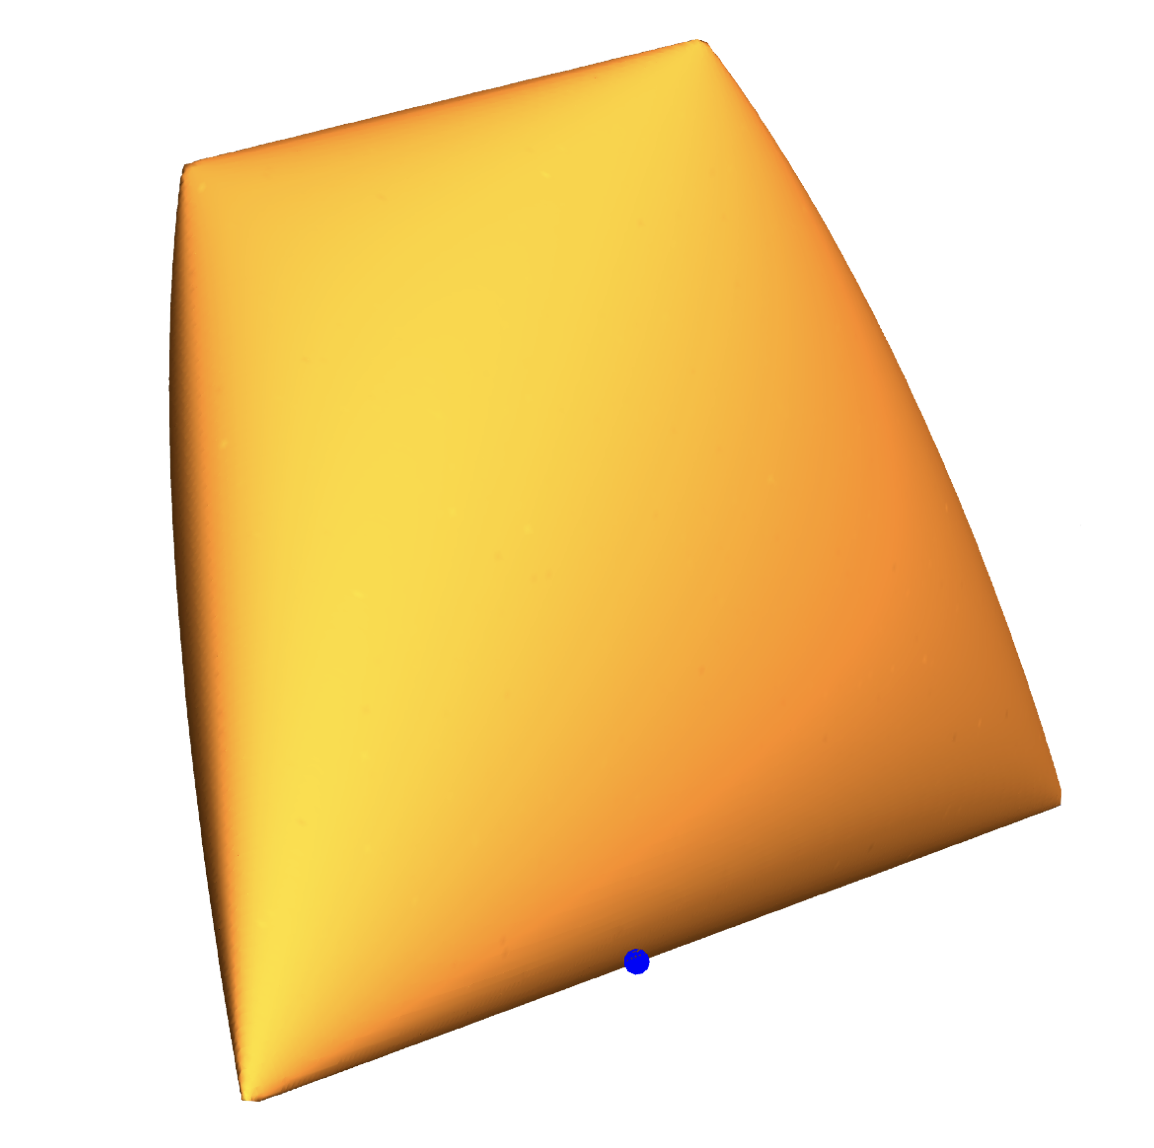
\includegraphics[width=0.5\linewidth]{images/spectrahedron-stride} 

}

\caption{An example spectrahedron.}\label{fig:SpectrahedronStride}
\end{figure}

Similarly, we say a matrix \(A \in \mathbb{S}^{n}\) is \textbf{positive definite} (PD) is its associated quadratic form is always positive, i.e.,
\[
x^\top A x > 0, \quad \forall x \in \mathbb{R}^{n}.
\]
We use \(\mathbb{S}^{n}_{++}\) to denote the set of \(n \times n\) PD matrices, and also write \(A \succ 0\) when the dimension is clear.

Below is set of equivalent characterizations of positive definite matrices.

\begin{lemma}[Positive Definite Matrices]
\protect\hypertarget{lem:PositiveDefinite}{}\label{lem:PositiveDefinite}

Let \(A \in \mathbb{S}^{n}\) be a symmetric matrix, the following statements are equivalent:

\begin{enumerate}
\def\labelenumi{\arabic{enumi}.}
\item
  A is positive definite.
\item
  \(x^\top A x > 0, \forall x \in \mathbb{R}^{n}\).
\item
  All eigenvalues of \(A\) are strictly positive.
\item
  All \(n\) leading principal minors of \(A\) are strictly positive.
\item
  The coefficients of \(p_A(\lambda)\) strictly alternate in sign, i.e., \((-1)^{n-k} p_k > 0\) for \(k=0,\dots,n-1\), where \(p_A(\lambda) = \det (A - \lambda \mathrm{I}_n)\) is the characteristics polynomial of \(A\).
\item
  There exists a factorization \(A = BB^\top\) with \(B\) square and nonsingular (full-rank).
\end{enumerate}

\end{lemma}

\textbf{Schur Complements}. A useful technique to check whether a matrix is positive (semi-)definite is to use the Schur Complements. Consider a block-partitioned matrix
\begin{equation}
M = \begin{bmatrix} A & B \\ B^\top& C \end{bmatrix},
\label{eq:block-mat-M}
\end{equation}
where \(A\) and \(C\) are symmetric matrices.
If \(A\) is invertible, then the Schur complement of \(A\) is
\[
M / A = C - B^\top A^{-1}B.
\]
Similarly, if \(C\) is invertible, then the Schur complement of \(C\) is
\[
M / C = A - B C^{-1}B^\top.
\]

We have the following result relating the Schur Complements to positive (semi-)definiteness.

\begin{proposition}[Schur Complements and PSD]
\protect\hypertarget{prp:SchurPSD}{}\label{prp:SchurPSD}

Consider the block-partitioned matrix \(M\) in \eqref{eq:block-mat-M},

\begin{itemize}
\item
  \(M\) is positive definite if and only if both \(A\) and \(M/A\) are positive definite:
  \[
  M \succ 0 \Leftrightarrow A \succ 0, M/A = C - B^\top A^{-1}B \succ 0.
  \]
\item
  \(M\) is positive definite if and only if both \(C\) and \(M/C\) are positive definite:
  \[
  M \succ 0 \Leftrightarrow C \succ 0, M/C = A - B C^{-1}B^\top\succ 0.
  \]
\item
  If \(A\) is positive definite, then \(M\) is positive semidefinite if and only if \(M/A\) is positive semidefinite:
  \[
  \text{If } A \succ 0, \text{ then } M \succeq 0 \Leftrightarrow M / A \succeq 0.
  \]
\item
  If \(C\) is positive definite, then \(M\) is positive semidefinite if and only if \(M/C\) is positive semidefinite:
  \[
  \text{If } C \succ 0, \text{ then } M \succeq 0 \Leftrightarrow M / C \succeq 0.
  \]
\end{itemize}

\end{proposition}

\hypertarget{geometric-properties}{%
\subsection{Geometric Properties}\label{geometric-properties}}

The set \(\mathbb{S}^{n}_{+}\) is a proper cone (cf.~Definition \ref{def:ProperCone}). Its interior is \(\mathbb{S}^{n}_{++}\). Under the inner product
\[
\langle A, B \rangle = \mathrm{tr}(AB^\top), \quad A,B \in \mathbb{R}^{n \times n},
\]
the PSD cone \(\mathbb{S}^{n}_{+}\) is self-dual.

Next we want to characterize the face of the PSD cone. We first present the following lemma which will turn out to be useful afterwards.

\begin{lemma}[Range of PSD Matrices]
\protect\hypertarget{lem:PSDRange}{}\label{lem:PSDRange}Let \(A,B \in \mathbb{S}^{n}_{+}\), then we have
\begin{equation}
\mathrm{Range}(A) \subseteq \mathrm{Range}(A + B),
\label{eq:Range-PSD}
\end{equation}
where \(\mathrm{Range}(A)\) denotes the span of the column vectors of \(A\).
\end{lemma}

\begin{proof}
For any symmetric matrix \(S\), we know
\[
\mathrm{Range}(S) = \mathrm{ker}(S)^{\perp}.
\]
Therefore, to prove \eqref{eq:Range-PSD}, it is equivalent to prove
\[
\mathrm{ker}(A) \supseteq \mathrm{ker}(A + B).
\]
Pick any \(u \in \mathrm{ker}(A + B)\), we have
\[
(A + B) u = 0 \Rightarrow u ^\top(A + B) u = 0 \Rightarrow u^\top A u + u^\top B u = 0 \Rightarrow u^\top A u = u^\top B u = 0,
\]
where the last derivation is due to \(A, B \succeq 0\). Now that we have \(u^\top A u = 0\), we claim that \(Au = 0\) must hold, i.e., \(u \in \mathrm{ker}(A)\). To see this, write
\[
u = \sum_{i=1}^n a_i v_i,
\]
where \(a_i = \langle u, v_i \rangle\) and \(v_i,i=1,\dots,n\) are the eigenvectors of \(A\) corresponding to eigenvalues \(\lambda_i,i=1,\dots,n\). Then we have
\[
Au = \sum_{i=1}^n a_i A v_i = \sum_{i=1}^n a_i \lambda_i v_i,
\]
and
\[
u^\top A u = \sum_{i=1}^n \lambda_i a_i^2 = 0.
\]
Since \(\lambda_i \geq 0, a_i^2 \geq 0\), we have
\[
\lambda_i a_i^2 = 0, \forall i = 1,\dots,n.
\]
This indicates that if \(\lambda_i > 0\), then \(a_i = 0\). Therefore, \(a_i\) can only be nonzero for \(\lambda_i = 0\), which leads to
\[
Au = \sum_{i=1}^n a_i \lambda_i v_i = 0.
\]
Therefore, \(u \in \mathrm{ker}(A)\), proving the result.
\end{proof}

Lemma \ref{lem:PSDRange} indicates that if \(A \succeq B\), then \(\mathrm{Range}(B) \subseteq \mathrm{Range}(A)\). What about the reverse?

\begin{lemma}[Extend Line Segment]
\protect\hypertarget{lem:Extension}{}\label{lem:Extension}Let \(A,B \in \mathbb{S}^{n}_{+}\), if \(\mathrm{Range}(B) \subseteq \mathrm{Range}(A)\), then there must exist \(C \in \mathbb{S}^{n}_{+}\) such that
\[
A \in (B,C),
\]
i.e., the line segment from \(B\) to \(A\) can be extended past \(A\) within \(\mathbb{S}^{n}_{+}\).
\end{lemma}

\begin{proof}
Since \(\mathrm{Range}(B) \subseteq \mathrm{Range}(A)\), we have
\[
\mathrm{ker}(A) \subseteq \mathrm{ker}(B).
\]
Now consider extending the line segment past \(A\) to
\[
C_{\alpha} = A + \alpha(A - B) = (1+\alpha) A - \alpha B,
\]
with some \(\alpha > 0\). We want to show that there exists \(\alpha > 0\) such that \(C_{\alpha} \succeq 0\).

Pick \(u \in \mathbb{R}^{n}\), then either \(u \in \mathrm{ker}(B)\) or \(u \not\in \mathrm{ker}(B)\). If \(u \in \mathrm{ker}(B)\), then
\[
u^\top C_{\alpha} u = (1+\alpha) u^\top A u - \alpha u^\top B u = (1+\alpha) u^\top A u \geq 0.
\]
If \(u \not\in \mathrm{ker}(B)\), then due to \(\mathrm{ker}(A) \subseteq \mathrm{ker}(B)\), we have \(u \not\in \mathrm{ker}(A)\) as well. As a result, we have
\begin{equation}
u^\top C_{\alpha} u = (1+\alpha) u^\top A u - \alpha u^\top B u = (1+\alpha) u^\top A u \lparen{ 1- \frac{\alpha}{1+\alpha} \frac{u^\top B u}{u^\top A u} }.
\label{eq:prove-extension-1}
\end{equation}
Since
\[
\max_{u: u \not\in \mathrm{ker}(A)} \frac{u^\top B u}{u^\top A u} \leq \frac{\lambda_{\max}(B)}{\lambda_{\min,>0}(A)},
\]
where \(\lambda_{\min,>0}(A)\) denotes the minimum positive eigenvalue of \(A\), we can always choose \(\alpha\) sufficiently small to make \eqref{eq:prove-extension-1} nonnegative. Therefore, there exists \(\alpha > 0\) such that \(C_{\alpha} \succeq 0\).
\end{proof}

In fact, from Lemma \ref{lem:PSDRange} we can induce a corollary.

\begin{corollary}[Range of PSD Matrices]
\protect\hypertarget{cor:PSDRange}{}\label{cor:PSDRange}Let \(A, B \in \mathbb{S}^{n}_{+}\), then we have
\[
\mathrm{Range}(A + B) = \mathrm{Range}(A) + \mathrm{Range}(B),
\]
with ``\(+\)'' the Minkowski sum.
\end{corollary}

\begin{exercise}
Let \(A,B \in \mathbb{S}^{n}_{+}\), show that \(\langle A, B \rangle = 0\) if and only if \(\mathrm{Range}(A) \perp \mathrm{Range}(B)\).
\end{exercise}

For a subset \(T \subseteq \mathbb{S}^{n}_{+}\), we use \(\mathrm{face}(T,\mathbb{S}^{n}_{+})\) to denote the smallest face of \(\mathbb{S}^{n}_{+}\) that contains \(T\). We first characterize the smallest face that contains a given PSD matrix, i.e., \(\mathrm{face}(A,\mathbb{S}^{n}_{+})\) for \(A\succeq 0\). Clearly, if \(A\) is PD, then \(\mathrm{face}(A, \mathbb{S}^{n}_{+}) = \mathbb{S}^{n}_{+}\) is the entire cone. If \(A\) is PSD but singular with rank \(r < n\), then \(A\) has the following spectral decomposition
\[
Q^\top A Q = \begin{bmatrix} \Lambda & 0 \\ 0 & 0 \end{bmatrix},
\]
where \(\Lambda \in \mathbb{S}^{r}_{++}\) is a diagonal matrix with the \(r\) nonzero eigenvalues of \(A\), and \(Q \in \mathrm{O}(n)\) is orthogonal. If
\[
A = \lambda B + (1-\lambda)C, \quad B,C \in \mathbb{S}^{n}_{+},\lambda \in (0,1),
\]
then multiplying both sides by \(Q^\top\) and \(Q\) we have
\[
\begin{bmatrix} \Lambda & 0 \\ 0 & 0 \end{bmatrix} = Q^\top A Q = \lambda Q^\top B Q + (1-\lambda) Q^\top C Q.
\]
Therefore, it must hold that
\[
Q^\top B Q = \begin{bmatrix} B_1 & 0 \\ 0 & 0 \end{bmatrix}, \quad Q^\top C Q = \begin{bmatrix} C_1 & 0 \\ 0 & 0 \end{bmatrix}, \quad B_1 \in \mathbb{S}^{r}_{+}, C_1 \in \mathbb{S}^{r}_{+},
\]
which is equivalent to
\[
B = Q \begin{bmatrix} B_1 & 0 \\ 0 & 0 \end{bmatrix} Q^\top, C = Q \begin{bmatrix} C_1 & 0 \\ 0 & 0 \end{bmatrix} Q^\top, \quad B_1 \in \mathbb{S}^{r}_{+}, C_1 \in \mathbb{S}^{r}_{+}.
\]
We conclude that \(\mathrm{face}(A,\mathbb{S}^{n}_{+})\) must contain the set
\begin{equation}
G:=  \left\{ Q \begin{bmatrix} X & 0 \\ 0 & 0 \end{bmatrix} Q^\top\ \middle\vert\ X \in \mathbb{S}^{r}_{+} \right\} .
\label{eq:face-of-A-psd}
\end{equation}

\begin{exercise}
Show that \(G\) in \eqref{eq:face-of-A-psd} is a face of \(\mathbb{S}^{n}_{+}\), i.e., (i) \(G\) is convex; (ii) \(u \in (x,y), u \in G, x,y \in \mathbb{S}^{n}_{+} \Rightarrow x,y \in G\).
\end{exercise}

As a result, we have \(\mathrm{face}(A,\mathbb{S}^{n}_{+}) = G\).

More general faces of the PSD cone \(\mathbb{S}^{n}_{+}\) can be characterized as follows (Theorem 3.7.1 in \citep{wolkowicz12book-sdp}).

\begin{theorem}[Faces of the PSD Cone]
\protect\hypertarget{thm:FacePSD}{}\label{thm:FacePSD}A set \(F \subseteq \mathbb{S}^{n}_{+}\) is a face if and only if there exists a subspace \(L \subseteq \mathbb{R}^{n}\) such that
\[
F = \{ X \in \mathbb{S}^{n}_{+} \mid \mathrm{Range}(X) \subseteq L \}.
\]
\end{theorem}

\begin{proof}
It is easy to prove the ``\textbf{If}'' direction using Lemma \ref{lem:PSDRange}.

First we show \(F\) is convex. Pick \(A,B \in F\). We have \(\mathrm{Range}(A) \subseteq L\) and \(\mathrm{Range}(B) \subseteq L\). Let \(v_1,\dots,v_m\) be a set of basis spanning \(L\). We have that, for any \(u \in \mathbb{R}^{n}\),
\begin{equation}
\begin{split}
A u \in L & \Rightarrow Au = \sum_{i=1}^m a_i v_i, \\
B u \in L & \Rightarrow Bu = \sum_{i=1}^m b_i v_i. 
\end{split}
\end{equation}
So for any \(\lambda \in [0,1]\), we have
\[
(\lambda A + (1-\lambda) B) u = \lambda Au + (1-\lambda) Bu = \sum_{i=1}^m (\lambda a_i + (1-\lambda) b_i ) v_i \in L,
\]
implying \(\lambda A + (1-\lambda) B \in F\) for any \(\lambda \in [0,1]\).

Now we show that:
\[
X \in (A,B), X \in F, A,B \in \mathbb{S}^{n}_{+} \Rightarrow A, B \in F.
\]
From \(X = \lambda A + (1-\lambda) B\) for some \(\lambda \in (0,1)\), and invoking Lemma \ref{lem:PSDRange}, we have
\begin{equation}
\begin{split}
\mathrm{Range}(X) & = \mathrm{Range}(\lambda A + (1-\lambda) B) \supseteq \mathrm{Range}(\lambda A) = \mathrm{Range}(A) \\
\mathrm{Range}(X) & = \mathrm{Range}(\lambda A + (1-\lambda) B) \supseteq \mathrm{Range}((1-\lambda) B) = \mathrm{Range}(B).
\end{split}
\end{equation}
Since \(\mathrm{Range}(X) \subseteq L\) due to \(X \in F\), we have
\[
\mathrm{Range}(A) \subseteq L, \quad \mathrm{Range}(B) \subseteq L,
\]
leading to \(A,B \in F\).

The proof for the ``\textbf{Only If}'' direction can be found in Theorem 3.7.1 of \citep{wolkowicz12book-sdp}.
\end{proof}

\hypertarget{semidefinite-programming}{%
\section{Semidefinite Programming}\label{semidefinite-programming}}

\hypertarget{spectrahedra}{%
\subsection{Spectrahedra}\label{spectrahedra}}

Recall the definition of a polyhedron in \eqref{eq:polyhedron}, i.e., a vector \(x\) constrained by finitely many linear inequalities. The feasible set of a Linear Program is a polyhedron.

Similarly, we define a \textbf{spectrahedron} as a set defined by finitely many \textbf{linear matrix inequalities} (LMIs). Spectrahedra are the feasible sets of Semidefinite Programs (SDPs).

A linear matrix inequality has the form
\[
A_0 + \sum_{i=1}^m A_i x_i \succeq 0,
\]
where \(A_i \in \mathbb{S}^{n},i=0,\dots,m\) are given symmetric matrices. Correspondingly, a spectrahedron is defined by finitely many LMIs.

\begin{definition}[Spectrahedron]
\protect\hypertarget{def:Spectrahedron}{}\label{def:Spectrahedron}A set \(S \subseteq \mathbb{R}^{m}\) is a spectrahedron if it has the form
\[
S =  \left\{ x \in \mathbb{R}^{m} \ \middle\vert\ A_0 + \sum_{i=1}^m x_i A_i \succeq 0 \right\} ,
\]
for given symmetric matrices \(A_0,A_1,\dots,A_m \in \mathbb{S}^{n}\).
\end{definition}

Note that there is no less of generality in defining a spectrahedron using a single LMI. For example, in the case of a set defined by two LMIs:
\[
S =  \left\{ x \in \mathbb{R}^{m} \ \middle\vert\ A_0 + \sum_{i=1}^m x_i A_i \succeq 0, B_0 + \sum_{i=1}^m x_i B_i \succeq 0  \right\} , A_i \in \mathbb{S}^{n}, B_i \in \mathbb{S}^{d},
\]
we can compress the two LMIs into a single LMI by putting \(A_i\) and \(B_i\) along the diagonal:
\[
S =  \left\{ x \in \mathbb{R}^{m} \ \middle\vert\ \begin{bmatrix} A_0 & \\ & B_0 \end{bmatrix} + \sum_{i=1}^m x_i \begin{bmatrix} A_i & \\ & B_i \end{bmatrix} \succeq 0  \right\} .
\]

Leveraging (5) of Lemma \ref{lem:PositiveSemidefinite}, we know that a PSD constraint is equivalent to weakly alternating signs of the characteristic polynomial of the given matrix. Therefore, a spectrahedron is defined by finitely many polynomial inequalities, i.e., a spectrahedron is a (convex) \textbf{basic semialgebraic set}, as seen in the following example \citep{blekherman12book-semidefinite}.

\begin{example}[Elliptic Curve]
\protect\hypertarget{exm:EllipticCurve}{}\label{exm:EllipticCurve}

Consider the spectrahedron in \(\mathbb{R}^{2}\) defined by
\[
 \left\{ (x,y) \in \mathbb{R}^{2} \ \middle\vert\ A(x,y) = \begin{bmatrix} x+1 & 0 & y \\ 0 & 2 & -x-1 \\ y & -x-1 & 2 \end{bmatrix} \succeq 0  \right\} .
\]
To obtain scalar inequalities defining the set, let
\[
p_A(\lambda) = \det (\lambda I - A(x,y)) = \lambda^3 + p_2 \lambda^2 + p_1 \lambda + p_0
\]
be the characteristic polynomial of \(A(x,y)\). \(A(x,y) \succeq 0\) is then equivalent to the coefficients weakly alternating in sign:
\begin{equation}
\begin{split}
p_2 & = -(x+5) \leq 0, \\
p_1 & = -x^2 + 2x - y^2 + 7 \geq 0, \\
p_0 & = -(3+ x -x^3 -3x^2 - 2y^2) \leq 0.
\end{split}
\end{equation}
We can use the following Matlab script to plot the set shown in Fig. \ref{fig:EllipticCurve}. (The code is also available at \href{https://github.com/ComputationalRobotics/Semidefinite-Examples}{here}.) As we can see, the spectrahedron is convex, but it is not a polyhedron.

\begin{Shaded}
\begin{Highlighting}[]
\VariableTok{x} \OperatorTok{=} \OperatorTok{{-}}\FloatTok{2}\OperatorTok{:}\FloatTok{0.01}\OperatorTok{:}\FloatTok{2}\OperatorTok{;} 
\VariableTok{y} \OperatorTok{=} \OperatorTok{{-}}\FloatTok{2}\OperatorTok{:}\FloatTok{0.01}\OperatorTok{:}\FloatTok{2}\OperatorTok{;} 
\NormalTok{[}\VariableTok{X}\OperatorTok{,}\VariableTok{Y}\NormalTok{] }\OperatorTok{=} \VariableTok{meshgrid}\NormalTok{(}\VariableTok{x}\OperatorTok{,}\VariableTok{y}\NormalTok{)}\OperatorTok{;}

\VariableTok{ineq} \OperatorTok{=}\NormalTok{ (}\OperatorTok{{-}}\VariableTok{X} \OperatorTok{{-}} \FloatTok{5} \OperatorTok{\textless{}=} \FloatTok{0}\NormalTok{) }\OperatorTok{\&} \OperatorTok{...}
\NormalTok{    (}\OperatorTok{{-}}\VariableTok{X}\OperatorTok{.\^{}}\FloatTok{2} \OperatorTok{+} \FloatTok{2}\OperatorTok{*}\VariableTok{X} \OperatorTok{{-}} \VariableTok{Y}\OperatorTok{.\^{}}\FloatTok{2} \OperatorTok{+} \FloatTok{7} \OperatorTok{\textgreater{}=}\FloatTok{0}\NormalTok{) }\OperatorTok{\&} \OperatorTok{...}
\NormalTok{    (}\FloatTok{3} \OperatorTok{+} \VariableTok{X} \OperatorTok{{-}} \VariableTok{X}\OperatorTok{.\^{}}\FloatTok{3} \OperatorTok{{-}} \FloatTok{3}\OperatorTok{*}\VariableTok{X}\OperatorTok{.\^{}}\FloatTok{2} \OperatorTok{{-}} \FloatTok{2}\OperatorTok{*}\VariableTok{Y}\OperatorTok{.\^{}}\FloatTok{2} \OperatorTok{\textgreater{}=} \FloatTok{0}\NormalTok{)}\OperatorTok{;}

\VariableTok{h} \OperatorTok{=} \VariableTok{pcolor}\NormalTok{(}\VariableTok{X}\OperatorTok{,}\VariableTok{Y}\OperatorTok{,}\VariableTok{double}\NormalTok{(}\VariableTok{ineq}\NormalTok{)) }\OperatorTok{;}
\VariableTok{h}\NormalTok{.}\VariableTok{EdgeColor} \OperatorTok{=} \SpecialStringTok{\textquotesingle{}none\textquotesingle{}} \OperatorTok{;}
\end{Highlighting}
\end{Shaded}

\begin{figure}

{\centering 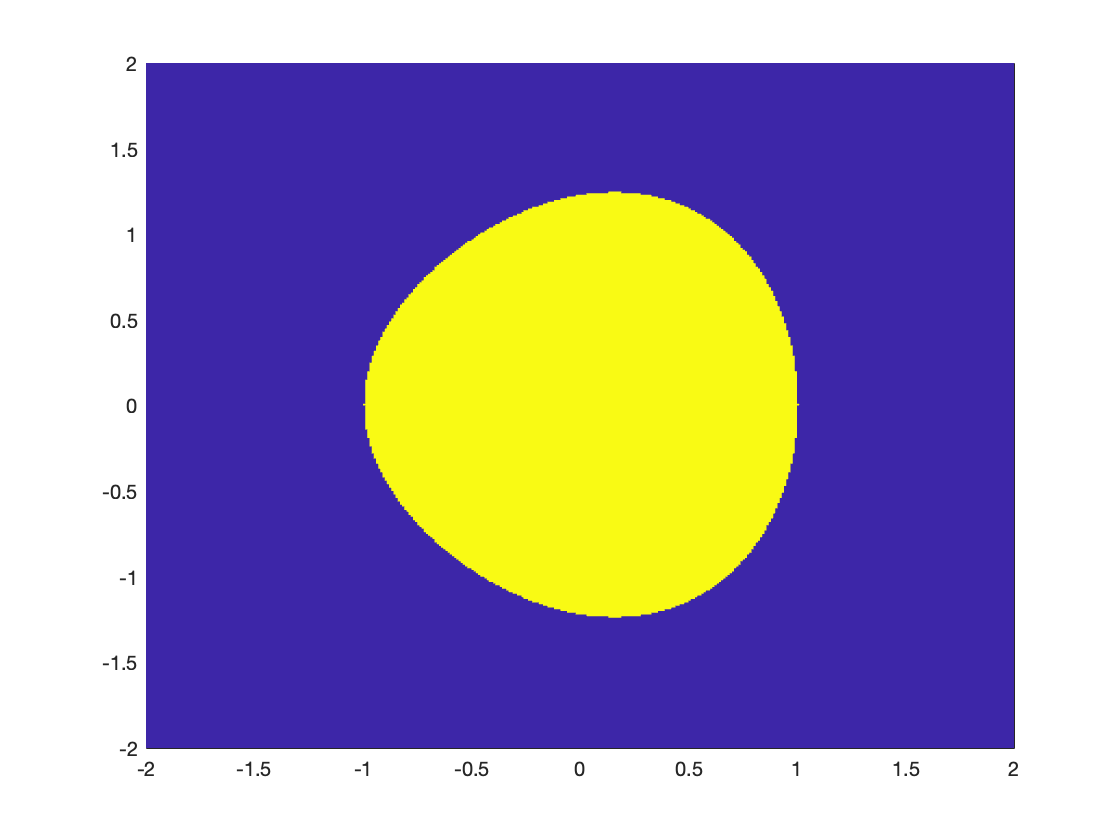
\includegraphics[width=0.6\linewidth]{images/elliptic_curve} 

}

\caption{Elliptic Curve.}\label{fig:EllipticCurve}
\end{figure}

\end{example}

We can use the same technique to visualize the elliptope, a spectrahedron that we will see again later when we study the MAXCUT problem.

\begin{example}[Elliptope]
\protect\hypertarget{exm:Elliptope}{}\label{exm:Elliptope}

Consider the 3D elliptope defined by
\[
 \left\{ (x,y,z) \in \mathbb{R}^{3} \ \middle\vert\ A(x,y,z) = \begin{bmatrix} 1 & x & y \\ x & 1 & z \\ y & z & 1 \end{bmatrix} \succeq 0 \right\} .
\]
The characteristic polynomial of \(A(x,y,z)\) is
\[
p_A(\lambda) = \lambda^3 - 3 \lambda^2 + (-x^2 - y^2 - z^2 + 3) \lambda + x^2 - 2 xyz + y^2 + z^2 -1. 
\]
The coefficients need to weakly alternative in sign, we have the inequalities
\begin{equation}
\begin{split}
-x^2 - y^2 - z^2 + 3 & \geq 0 \\
x^2 - 2 xyz + y^2 + z^2 -1 & \leq 0
\end{split}
\end{equation}

Using the Matlab script \href{https://github.com/ComputationalRobotics/Semidefinite-Examples/blob/main/elliptope.m}{here}, we generate the following plot.

\begin{figure}

{\centering 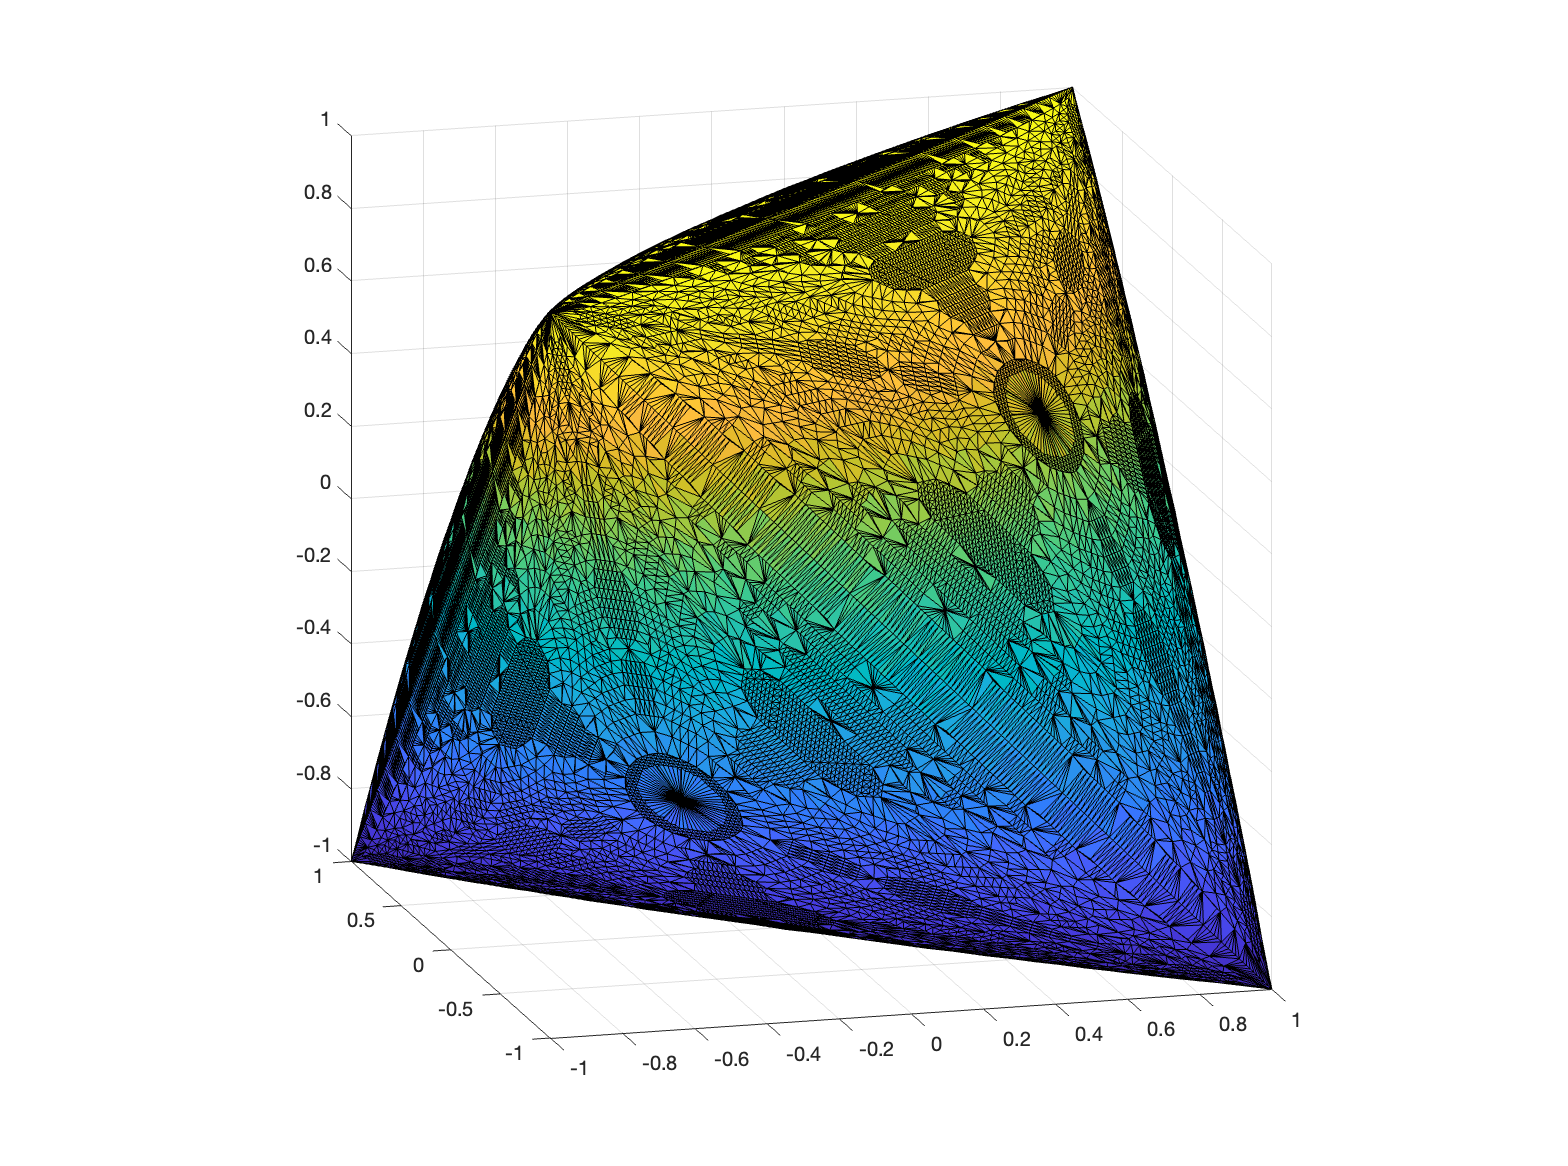
\includegraphics[width=0.8\linewidth]{images/elliptope} 

}

\caption{Elliptope.}\label{fig:Elliptope}
\end{figure}

\end{example}

Another example is provided in Fig. \ref{fig:SpectrahedronStride}.

\hypertarget{formulation-and-duality}{%
\subsection{Formulation and Duality}\label{formulation-and-duality}}

Semidefinite programs (SDPs) are linear optimization problems over spectrahedra. A standard SDP in \textbf{primal} form is written as
\begin{equation}
\boxed{
\begin{split}
p^\star = \min_{X \in \mathbb{S}^{n}} & \quad \langle C, X \rangle \\
\mathrm{s.t.}& \quad \mathcal{A}(X) = b, \\
& \quad X \succeq 0
\end{split}
}
\label{eq:SDP-P}
\end{equation}
where \(C \in \mathbb{S}^{n}\), \(b \in \mathbb{R}^{m}\), and the linear map \(\mathcal{A}: \mathbb{S}^{n} \rightarrow \mathbb{R}^{m}\) is defined as
\[
\mathcal{A}(X) := \begin{bmatrix} \langle A_1, X \rangle \\
\vdots \\ \langle A_i, X \rangle \\ \langle A_m, X \rangle \end{bmatrix}.
\]
Recall that \(\langle C, X \rangle = \mathrm{tr}(CX)\). The feasible set of \eqref{eq:SDP-P} is the intersection of the PSD cone (\(\mathbb{S}^{n}_{+}\)) and the affine subspace defined by \(\mathcal{A}(X) = b\).

Closely related to the primal SDP \eqref{eq:SDP-P} is the \textbf{dual} problem
\begin{equation}
\boxed{
\begin{split}
d^\star = \max_{y \in \mathbb{R}^{m}} & \quad \langle b, y \rangle \\
\mathrm{s.t.}& \quad C - \mathcal{A}^* (y) \succeq 0
\end{split}
}
\label{eq:SDP-D}
\end{equation}
where \(\mathcal{A}^{*}: \mathbb{R}^{m} \rightarrow \mathbb{S}^{n}\) is the \textbf{adjoint} map defined as
\[
\mathcal{A}^*(y) := \sum_{i=1}^m y_i A_i.
\]
Observe how the primal-dual SDP pair \eqref{eq:SDP-P}-\eqref{eq:SDP-D} parallels the primal-dual LP pair \eqref{eq:primal-lp}-\eqref{eq:dual-lp}.

\textbf{Weak duality}. We have a similar weak duality between the primal and dual. Pick any \(X\) that is feasible for the primal \eqref{eq:SDP-P} and \(y\) that is feasible for the dual \eqref{eq:SDP-D}, we have
\[
\boxed{\langle C, X \rangle - \langle b, y \rangle = \langle C, X \rangle - \langle \mathcal{A}(X), y \rangle = \langle C - \mathcal{A}^* (y), X \rangle \geq 0,}
\]
where the last inequality holds because both \(C - \mathcal{A}^*(y)\) and \(X\) are positive semidefinite. As a result, we have the weak duality
\[
d^\star \leq p^\star.
\]

Similar to the LP case, we will denote \(p^\star = +\infty\) if the primal is infeasible, \(p^\star = - \infty\) if the primal is unbounded below. We will denote \(d^\star = +\infty\) if the dual is unbounded above, and \(d^\star = -\infty\) if the dual is infeasible. We say the primal (or the dual) is \textbf{solvable} if it admits optimizers. We denote \(p^\star - d^\star\) as the \textbf{duality gap}.

Recall Theorem \ref{thm:LPStrongDuality} states that in LP, if at least one of the primal and dual is feasible, then strong duality holds (i.e., \(p^\star = d^\star = \{\pm \infty, \text{finite} \}\)). Unfortunately, this does not carry over to SDPs. Let us provide several examples.

\begin{example}[Failure of SDP Strong Duality]
\protect\hypertarget{exm:FailureSDPDuality}{}\label{exm:FailureSDPDuality}The first example, from \citep{ramana97mp-exact}, shows that even if both primal and dual are feasible, there could exist a nonzero duality gap. Consider the following SDP pair for some \(\alpha \geq 0\)
\[
\begin{cases}
\min_{X \in \mathbb{S}^{3}} & \alpha X_{11} \\
\mathrm{s.t.}& X_{22} = 0 \\
& X_{11} + 2 X_{23} = 1 \\
& \begin{bmatrix} X_{11} & X_{12} & X_{13} \\
* & X_{22} & X_{23} \\
* & * & X_{33} \end{bmatrix} \succeq 0 
\end{cases}, 
\begin{cases}
\max_{y \in \mathbb{R}^{2}} & y_2 \\
\mathrm{s.t.}& \begin{bmatrix} \alpha & 0 & 0 \\ 0 & 0 & 0 \\ 0 & 0 & 0 \end{bmatrix} \succeq \begin{bmatrix} y_2 & 0 & 0 \\ 0 & y_1 & y_2 \\ 0 & y_2 & 0 \end{bmatrix}
\end{cases}
\]
To examine the primal feasible set, let us pick the bottom-right \(2\times 2\) submatrix of \(X\). The determinant of this submatrix needs to be nonnegative (due to (4) of Lemma \ref{lem:PositiveSemidefinite}):
\[
X_{22} X_{33} - X_{23}^2 \geq 0.
\]
Because \(X_{22} = 0\), we have \(X_{23} = 0\) and hence \(X_{11} = 1\). Therefore, \(p^\star = \alpha\) is attained.

To examine the dual feasible set, pick the bottom-right \(2 \times 2\) submatrix of
\[
\begin{bmatrix} \alpha - y_2 & 0 & 0 \\ 0 & - y_1 & -y_2 \\ 0 & -y_2 & 0 \end{bmatrix} \succeq 0,
\]
we have \(y_2 = 0\). As a result, \(d^\star = 0\), and strong duality fails.

The second example, from \citep{todd01an-semidefinite}, shows that the duality gap can even be infinite. Consider the primal-dual SDP
\[
\begin{cases}
\min_{X \in \mathbb{S}^{2}} & 0 \\
\mathrm{s.t.}& X_{11} = 0 \\
& X_{12} = 1 \\
& \begin{bmatrix} X_{11} & X_{12} \\ * & X_{22} \end{bmatrix} \succeq 0
\end{cases},
\begin{cases}
\max_{y \in \mathbb{R}^{2}} & 2 y_2 \\
\mathrm{s.t.}& \begin{bmatrix} - y_1 & - y_2 \\ - y_2 & 0 \end{bmatrix} \succeq 0 
\end{cases}
\]
Clearly, the primal is infeasible because
\[
\begin{bmatrix} 0 & 1 \\ 1 & X_{22} \end{bmatrix}
\]
can never be PSD. So \(p^\star = + \infty\). The dual problem, however, is feasible. From the PSD constraint we have \(y_2 = 0\) and \(d^\star = 0\). Therefore, the duality gap is infinite.

The third example, from \citep{todd01an-semidefinite}, shows that even when the duality gap is zero, the primal or dual problem may not admit optimizers. Consider the primal-dual SDP
\[
\begin{cases}
\min_{X \in \mathbb{S}^{2}} & 2 X_{12} \\
\mathrm{s.t.}& - X_{11} = -1 \\
& - X_{22} = 0 \\
& \begin{bmatrix} X_{11} & X_{12} \\ * & X_{22} \end{bmatrix} \succeq 0 
\end{cases},
\begin{cases}
\max_{y \in \mathbb{R}^{2}} & - y_1 \\
\mathrm{s.t.}& \begin{bmatrix} y_1 & 1 \\ 1 & y_2 \end{bmatrix} \succeq 0
\end{cases}
\]
To examine the primal feasible set, we have
\[
\begin{bmatrix} 1 & X_{12} \\ X_{12} & 0 \end{bmatrix} \succeq 0
\]
implies \(X_{12} = 0\). Hence the primal feasible set only has one point and \(p^\star = 0\). The dual feasible set reads
\[
y_1 y_2 \geq 1,\quad  y_1 \geq 0, \quad y_2 \geq 0,
\]
and we want to minimize \(y_1\). Clearly, \(d^\star = 0\) but it is not attainable. Therefore, strong duality holds but the dual problem is not solvable.

A Matlab script that passes these three examples to SDP solvers can be found \href{https://github.com/ComputationalRobotics/Semidefinite-Examples/blob/main/failure_strong_duality.m}{here}.
\end{example}

The examples above are somewhat ``pathological'' and they show that SDPs in general can be more complicated that LPs. It turns out, with the addition of \textbf{Slater's condition}, i.e., \textbf{strict feasibility} of the primal and dual, we can recover nice results parallel to those of LP.

\begin{theorem}[SDP Strong Duality]
\protect\hypertarget{thm:SDPStrongDuality}{}\label{thm:SDPStrongDuality}Assume both the primal SDP \eqref{eq:SDP-P} and the dual SDP \eqref{eq:SDP-D} are \emph{strictly feasible}, i.e., there exists \(X \succ 0\) such that \(\mathcal{A}(X)=b\) for the primal and there exists \(y \in \mathbb{R}^{m}\) such that \(C - \mathcal{A}^* (y) \succ 0\) for the dual, then strong duality holds, i.e., both problems are solvable and admit optimizers, and \(p^\star = d^\star\) equals to some finite number.

Further, a pair of primal-dual feasible points \((X,y)\) is optimal if and only if
\[
\langle C, X \rangle = \langle b, y \rangle \Leftrightarrow \langle C - \mathcal{A}^* (y), X \rangle = 0 \Leftrightarrow (C - \mathcal{A}^* (y)) X = 0.
\]
\end{theorem}

One can relax the requirement of both primal and dual being strictly feasible to only one of them being strictly feasible, and similar results would hold. Precisely, if the primal is bounded below and strictly feasible, then \(p^\star = d^\star\) and the dual is solvable. If the dual is bounded above and strictly feasible, then \(p^\star = d^\star\) and the primal is solvable \citep{nie23book-moment}.

\begin{example}[SDP Strong Duality]
\protect\hypertarget{exm:SuccessSDPDuality}{}\label{exm:SuccessSDPDuality}Consider the following primal-dual SDP pair
\[
\begin{cases}
\min_{X \in \mathbb{S}^{2}} & 2 X_{11} + 2 X_{12} \\
\mathrm{s.t.}& X_{11} + X_{22} = 1 \\
& \begin{bmatrix} X_{11} & X_{12} \\ * & X_{22} \end{bmatrix} \succeq 0 
\end{cases},
\begin{cases}
\max_{y \in \mathbb{R}^{}} & y \\
\mathrm{s.t.}& \begin{bmatrix} 2 - y & 1 \\ 1 & - y \end{bmatrix} \succeq 0
\end{cases}
\]
Choose
\[
X = \begin{bmatrix} 0.5 & 0 \\ 0 & 0.5 \end{bmatrix} \succ 0
\]
we see the primal is strictly feasible.
Choose \(y = -1\), we have
\[
\begin{bmatrix} 3 & 1 \\ 1 & 1 \end{bmatrix} \succ 0
\]
and the dual is strictly feasible. Therefore, strong duality holds.

In this case, pick the pair of primal-dual feasible points
\[
X^\star = \begin{bmatrix} \frac{2 - \sqrt{2}}{4} & - \frac{1}{2 \sqrt{2}} \\ - \frac{1}{2 \sqrt{2}} & \frac{2 + \sqrt{2}}{4} \end{bmatrix}, \quad y^\star = 1 - \sqrt{2},
\]
we have
\[
\langle C, X^\star \rangle = 1-\sqrt{2} = \langle b, y^\star \rangle,
\]
and both \(X^\star\) and \(y^\star\) are optimal.
\end{example}

\hypertarget{geometric-properties-1}{%
\subsection{Geometric Properties}\label{geometric-properties-1}}

\hypertarget{software-for-conic-optimization}{%
\section{Software for Conic Optimization}\label{software-for-conic-optimization}}

Linear optimization over the nonnegative orthant (\(\mathbb{R}^{n}_{+}\)), the second-order cone (\(\mathcal{Q}_{n}\)), and the positive semidefinite cone (\(\mathbb{S}^{n}_{+}\)) forms the foundation of modern convex optimization, commonly referred to as conic optimization. These three types of cones are self-dual, and there exist efficient algorithms to solve the convex optimization problems. Popular solvers include SDPT3, SeDuMi, MOSEK, and SDPNAL+.

In this section, we introduce how we should ``talk to'' the numerical solvers for conic optimization, i.e., how should we pass a mathematically written conic optimization to a numerical solver. Note that in many cases, this ``transcription'' can be done by programming packages such as CVX, CVXPY, YALMIP etc., but I think it is important to understand the standard interface of numerical solvers because (i) it reinforces our understanding of the mathematical basics, (ii) it gets us closer to designing custom numerical solvers for specific problems, (iii) if you are a heavy convex optimization user you will realize that many of the programming packages are not ``efficient'' in transcribing the original optimization problem (but they are indeed very general). I have had cases where solving the conic optimization takes a few minutes but transcribing the problem to the solver takes half an hour.

We will use the SeDuMi format as an example. Consider the following general linear convex optimization problem
\begin{equation}
\begin{split}
\max_{y \in \mathbb{R}^{m}} & \quad b^\top y \\
\mathrm{s.t.}& \quad Fy = g \\
& \quad f \geq Gy \\
& \quad h_i^\top y + \tau_i \geq \Vert H_i y + p_i \Vert_2, i=1,\dots,r \\
& \quad B_{j,0} + \sum_{k=1}^m y_k B_{j,k} \succeq 0, j=1,\dots,s,
\end{split}
\label{eq:general-convex-sedumi}
\end{equation}
for given matrices and vectors
\[
F \in \mathbb{R}^{\ell_1 \times m},G \in \mathbb{R}^{\ell_2 \times m},H_i \in \mathbb{R}^{l_i \times m}, B_{j,k} \in \mathbb{S}^{n_j}, h_i \in \mathbb{R}^{m}, p_i \in \mathbb{R}^{l_i}, \tau_i \in \mathbb{R}^{}, g \in \mathbb{R}^{\ell_1},f \in \mathbb{R}^{\ell_2}.
\]
Define the linear function
\[
\phi(y):= \left(Fy, Gy, \begin{bmatrix} - h_1^\top y \\ - H_1 y \end{bmatrix}, \dots, \begin{bmatrix} - h_r^\top y \\ - H_r y \end{bmatrix}, - \sum_{k=1}^m y_k B_{1,k}, \dots,- \sum_{k=1}^m y_k B_{s,k} \right),
\]
which is a linear map from \(\mathbb{R}^{m}\) to the vector space of Cartesian products
\[
V:= \mathbb{R}^{\ell_1} \times \mathbb{R}^{\ell_2} \times \mathbb{R}^{l_1+1} \times \dots \times \mathbb{R}^{l_r + 1} \times \mathbb{S}^{n_1}\times \dots \times \mathbb{S}^{n_s}.
\]
A vector \(X \in V\) can be written as a tuple
\[
X = (x_1,x_2,\mathrm{x}_1,\dots,\mathrm{x}_r,X_1,\dots,X_s).
\]
Given another vector \(Y \in V\)
\[
X = (y_1,y_2,\mathrm{y}_1,\dots,\mathrm{y}_r,Y_1,\dots,Y_s),
\]
the inner product between \(X\) and \(Y\) is defined as
\[
\langle X, Y \rangle = \langle x_1, y_2 \rangle + \langle x_2, y_2 \rangle + \sum_{i=1}^r \langle \mathrm{x}_i, \mathrm{y}_i \rangle + \sum_{j=1}^s \langle X_j, Y_j \rangle.
\]

Let \(\mathcal{K}\) be the Cartesian product of the free cone, the nonnegative orthant, the second-order cone, and the PSD cone
\[
\mathcal{K}:= \mathbb{R}^{\ell_1} \times \mathbb{R}^{\ell_2}_{+} \times \mathcal{Q}_{l_1} \times \dots \times \mathcal{Q}_{l_r} \times \mathbb{S}^{n_1}_{+} \times \dots \times \mathbb{S}^{n_s}_{+}.
\]
Its dual cone is
\[
\mathcal{K}^* = \{0\}^{\ell_1} \times \times \mathbb{R}^{\ell_2}_{+} \times \mathcal{Q}_{l_1} \times \dots \times \mathcal{Q}_{l_r} \times \mathbb{S}^{n_1}_{+} \times \dots \times \mathbb{S}^{n_s}_{+}.
\]
Note that all the cones there are self-dual except the free cone whose dual is the zero point. Then denote
\[
C := \left( g,f,\begin{bmatrix} \tau_1 \\ p_1 \end{bmatrix},\dots,\begin{bmatrix} \tau_r \\ p_r \end{bmatrix},B_{1,0},\dots,B_{s,0} \right) \in V,
\]
we have that the original optimization \eqref{eq:general-convex-sedumi} is simply the following dual conic problem
\begin{equation}
\max_{y \in \mathbb{R}^{m}} \{ b^\top y \mid C - \phi(y) \in \mathcal{K}^* \}.
\label{eq:dual-conic}
\end{equation}
The linear map \(\phi(y)\) can be written as
\[
\phi(y) = y_1 A_1 + \dots, y_m A_m
\]
for vectors \(A_1,\dots,A_m\) in the space \(V\). Therefore, the primal problem to \eqref{eq:dual-conic} is
\begin{equation}
\min_{X \in V} \{ \langle C, X \rangle \mid \langle A_i, X \rangle=b_i,i=1,\dots,m,X \in \mathcal{K} \}.
\label{eq:primal-conic}
\end{equation}

Let us practice an example from \citep{nie23book-moment}.

\begin{example}[SeDuMi Example]
\protect\hypertarget{exm:SeDuMiExample}{}\label{exm:SeDuMiExample}Consider the following optimization problem as an instance of \eqref{eq:general-convex-sedumi}:
\begin{equation}
\begin{split}
\max_{y \in \mathbb{R}^{3}} & \quad y_3 - y_1 \\
\mathrm{s.t.}& \quad y_1 + y_2 + y_3 = 3\\
& \quad -1 \geq -y_1 - y_2 \\
& \quad -1 \geq -y_2 - y_3 \\
& \quad y_1 + y_3 \geq \sqrt{(y_1-1)^2 + y_2^2 + (y_3 -1)^2} \\
& \quad \begin{bmatrix} 1 & y_1 & y_2 \\ y_1 & 2 & y_3 \\ y_2 & y_3 & 3 \end{bmatrix} \succeq 0
\end{split}
\label{eq:sedumi-example}
\end{equation}
Clearly we have \(b = (-1,0,1)\). The linear map \(\phi(y)\) is
\[
\phi(y) = \left( y_1+y_2+y_3,\begin{bmatrix} -y_1 - y_2 \\ - y_2 - y_3 \end{bmatrix}, \begin{bmatrix} - y_1 - y_3 \\ -y_1 \\ -y_2 \\ -y_3 \end{bmatrix}, \begin{bmatrix} 0 & -y_1 & -y_2 \\ -y_1 & 0 & -y_3 \\ -y_2 & -y_3 & 0 \end{bmatrix} \right).
\]
The vector space \(V=\mathbb{R}^{} \times \mathbb{R}^{2} \times \mathbb{R}^{4} \times \mathbb{S}^{3}\), and the cone \(\mathcal{K}\) is
\[
\mathcal{K}= \mathbb{R}^{} \times \mathbb{R}^{2}_{+} \times \mathcal{Q}_3 \times \mathbb{S}^{3}_{+}.
\]
The vectors \(A_1,A_2,A_3\) are
\begin{equation}
\begin{split}
A_1 &= \left( 1,\begin{bmatrix}-1\\0\end{bmatrix}, \begin{bmatrix}-1\\-1\\0\\0\end{bmatrix},\begin{bmatrix}0&-1&0\\-1&0&0\\0&0&0\end{bmatrix} \right)\\
A_2 &= \left( 1,\begin{bmatrix}-1\\-1\end{bmatrix}, \begin{bmatrix}0\\0\\-1\\0\end{bmatrix},\begin{bmatrix}0&0&-1\\0&0&0\\-1&0&0\end{bmatrix} \right)\\
A_3 &= \left( 1,\begin{bmatrix}0\\-1\end{bmatrix}, \begin{bmatrix}-1\\0\\0\\-1\end{bmatrix},\begin{bmatrix}0&0&0\\0&0&-1\\0&-1&0\end{bmatrix} \right).
\end{split}
\end{equation}
The vector \(C\) is
\[
C = \left( 3,\begin{bmatrix}-1\\-1\end{bmatrix}, \begin{bmatrix}0\\-1\\0\\-1\end{bmatrix},\begin{bmatrix}1&0&0\\0&2&0\\0&0&3\end{bmatrix} \right).
\]

To input this problem to SeDuMi, we only need to provide the data \((A,b,C)\) together with the description of the cones \(\mathcal{K}\).

\begin{Shaded}
\begin{Highlighting}[]
\CommentTok{\% describe dimensions of the cones}
\VariableTok{K}\NormalTok{.}\VariableTok{f} \OperatorTok{=} \FloatTok{1}\OperatorTok{;} \CommentTok{\% free cone}
\VariableTok{K}\NormalTok{.}\VariableTok{l} \OperatorTok{=} \FloatTok{2}\OperatorTok{;} \CommentTok{\% nonnegative orthant}
\VariableTok{K}\NormalTok{.}\VariableTok{q} \OperatorTok{=} \FloatTok{4}\OperatorTok{;} \CommentTok{\% second order cone}
\VariableTok{K}\NormalTok{.}\VariableTok{s} \OperatorTok{=} \FloatTok{3}\OperatorTok{;} \CommentTok{\% psd cone}

\CommentTok{\% provide A,b,c}
\VariableTok{c} \OperatorTok{=}\NormalTok{ [}\FloatTok{3}\OperatorTok{,{-}}\FloatTok{1}\OperatorTok{,{-}}\FloatTok{1}\OperatorTok{,}\FloatTok{0}\OperatorTok{,{-}}\FloatTok{1}\OperatorTok{,}\FloatTok{0}\OperatorTok{,{-}}\FloatTok{1}\OperatorTok{,}\FloatTok{1}\OperatorTok{,}\FloatTok{0}\OperatorTok{,}\FloatTok{0}\OperatorTok{,}\FloatTok{0}\OperatorTok{,}\FloatTok{2}\OperatorTok{,}\FloatTok{0}\OperatorTok{,}\FloatTok{0}\OperatorTok{,}\FloatTok{0}\OperatorTok{,}\FloatTok{3}\NormalTok{]}\OperatorTok{;}
\VariableTok{b} \OperatorTok{=}\NormalTok{ [}\OperatorTok{{-}}\FloatTok{1}\OperatorTok{,}\FloatTok{0}\OperatorTok{,}\FloatTok{1}\NormalTok{]}\OperatorTok{;}
\VariableTok{A} \OperatorTok{=}\NormalTok{ [}
    \FloatTok{1}\OperatorTok{,{-}}\FloatTok{1}\OperatorTok{,}\FloatTok{0}\OperatorTok{,{-}}\FloatTok{1}\OperatorTok{,{-}}\FloatTok{1}\OperatorTok{,}\FloatTok{0}\OperatorTok{,}\FloatTok{0}\OperatorTok{,}\FloatTok{0}\OperatorTok{,{-}}\FloatTok{1}\OperatorTok{,}\FloatTok{0}\OperatorTok{,{-}}\FloatTok{1}\OperatorTok{,}\FloatTok{0}\OperatorTok{,}\FloatTok{0}\OperatorTok{,}\FloatTok{0}\OperatorTok{,}\FloatTok{0}\OperatorTok{,}\FloatTok{0}\OperatorTok{;}
    \FloatTok{1}\OperatorTok{,{-}}\FloatTok{1}\OperatorTok{,{-}}\FloatTok{1}\OperatorTok{,}\FloatTok{0}\OperatorTok{,}\FloatTok{0}\OperatorTok{,{-}}\FloatTok{1}\OperatorTok{,}\FloatTok{0}\OperatorTok{,}\FloatTok{0}\OperatorTok{,}\FloatTok{0}\OperatorTok{,{-}}\FloatTok{1}\OperatorTok{,}\FloatTok{0}\OperatorTok{,}\FloatTok{0}\OperatorTok{,}\FloatTok{0}\OperatorTok{,{-}}\FloatTok{1}\OperatorTok{,}\FloatTok{0}\OperatorTok{,}\FloatTok{0}\OperatorTok{;}
    \FloatTok{1}\OperatorTok{,}\FloatTok{0}\OperatorTok{,{-}}\FloatTok{1}\OperatorTok{,{-}}\FloatTok{1}\OperatorTok{,}\FloatTok{0}\OperatorTok{,}\FloatTok{0}\OperatorTok{,{-}}\FloatTok{1}\OperatorTok{,}\FloatTok{0}\OperatorTok{,}\FloatTok{0}\OperatorTok{,}\FloatTok{0}\OperatorTok{,}\FloatTok{0}\OperatorTok{,}\FloatTok{0}\OperatorTok{,{-}}\FloatTok{1}\OperatorTok{,}\FloatTok{0}\OperatorTok{,{-}}\FloatTok{1}\OperatorTok{,}\FloatTok{0}
\NormalTok{    ]}\OperatorTok{;}

\CommentTok{\% solve using sedumi}
\NormalTok{[}\VariableTok{xopt}\OperatorTok{,}\VariableTok{yopt}\OperatorTok{,}\VariableTok{info}\NormalTok{] }\OperatorTok{=} \VariableTok{sedumi}\NormalTok{(}\VariableTok{A}\OperatorTok{,}\VariableTok{b}\OperatorTok{,}\VariableTok{c}\OperatorTok{,}\VariableTok{K}\NormalTok{)}\OperatorTok{;}
\end{Highlighting}
\end{Shaded}

Note that in providing \(A\), we vectorize each \(A_i\) and place it along the \(i\)-th row of the matrix \(A\).
The above Matlab script gives us the optimal solution
\[
y^\star = (0,1,2).
\]
To run the \href{https://github.com/ComputationalRobotics/Semidefinite-Examples/blob/main/sedumi_example.m}{code}, make sure you download \href{https://github.com/sqlp/sedumi}{SeDuMi} and add that to your Matlab path.
\end{example}

\hypertarget{interior-point-algorithm}{%
\section{Interior Point Algorithm}\label{interior-point-algorithm}}

A nice property of semidefinite optimization is that it can be solved in polynomial time. The algorithm of choice for solving SDPs is called an \textbf{interior point method} (IPM), which is also what popular SDP solvers like SeDuMI, MOSEK, and SDPT3 implement under the hood.

Although it can be difficult to implement an SDP solver as efficient and robust as MOSEK (as it requires many engineering wisdom), it is surprisingly simple to sketch out the basic algorithmic framework, as it is based on \href{https://en.wikipedia.org/wiki/Newton\%27s_method\#:~:text=14\%20External\%20links-,Description,the\%20method\%20can\%20be\%20iterated.}{Newton's method for solving a system of nonlinear equations}. Before I introduce you the basic algorithm, let me review two useful preliminaries.

Newton's Method

Given a function \(f: \mathbb{R}^{} \rightarrow \mathbb{R}^{}\) that is continuously differentiable, Newton's method is designed to find a root of \(f(x) = 0\). Given an initial iterate \(x^{(0)}\), Newton's method works as follows
\[
x^{(k+1)} = x^{(k)} - \frac{f(x^{(k)})}{f'(x^{(k)})},
\]
where \(f'(x^{(k)})\) denotes the derivative of \(f\) at the current iterate \(x^{(k)}\). This simple algorithm is indeed (in my opinion) the most important foundation of modern numerical optimization \citep{nocedal99book-numerical}. Under mild conditions, Newton's method has at least quadratic convergence rate, that is to say, if \(|x^{(k)} - x^\star| = \epsilon\), then \(|x^{(k+1)} - x^\star| = O(\epsilon^2)\). Of course, there exist pathological cases where even linear convergence is not guaranteed (e.g., when \(f'(x^\star) = 0\)).

Newton's method can be generalized to find a point at which multiple functions vanish simultaneously. Given a function \(F: \mathbb{R}^{n} \rightarrow \mathbb{R}^{n}\) that is continuously differentiable, and an initial iterate \(x^{(0)}\), Newton's method reads
\begin{equation}
x^{(k+1)} = x^{(k)} - J_F(x^{(k)})^{-1}F(x^{(k)}),
\label{eq:newton-method-vector}
\end{equation}
where \(J_F(\cdot)\) denotes the Jacobian of \(F\). Iteration \eqref{eq:newton-method-vector} is equivalent to
\begin{equation}
\begin{split}
J_F(x^{(k)}) \Delta x^{(k)} & = - F(x^{(k)}) \\
x^{(k+1)} & = x^{(k)} + \Delta x^{(k)}
\end{split}
\label{eq:newton-method-vector-1}
\end{equation}
i.e., one first solves a linear system of equations to find an update direction \(\Delta x^{(k)}\), and then take a step along the direction.

As we will see, IPMs for solving SDPs can be interpreted as applying Newton's method to the perturbed KKT optimality conditions.

We introduce another useful preliminary about the symmetric Kronecker product.

Symmetric Vectorization and Kronecker Product

Consider a linear operator on \(\mathbb{R}^{n \times n}\):
\begin{equation}
\begin{split}
\mathbb{R}^{n \times n} & \rightarrow \mathbb{R}^{n \times n} \\
K & \mapsto N K M^\top
\end{split}
\label{eq:linear-opt-Rn}
\end{equation}
where \(N,M \in \mathbb{R}^{n \times n}\) are given square matrices. This linear map is equivalent to
\begin{equation}
\begin{split}
\mathbb{R}^{n^2} & \rightarrow \mathbb{R}^{n^2} \\
\mathrm{vec}(K) & \mapsto (M \otimes N) \mathrm{vec}(K)
\end{split}
\label{eq:linear-opt-Rn-kron}
\end{equation}
where \(\otimes\) denotes the usual kronecker product.

Symmetric vectorization and kronecker product is to generalize the above linear map on \(\mathbb{R}^{n \times n}\) to \(\mathbb{S}^{n}\).

Consider a linear operator on \(\mathbb{S}^{n}\):
\begin{equation}
\begin{split}
\mathbb{S}^{n} & \rightarrow \mathbb{S}^{n} \\
K & \mapsto \frac{1}{2} \left( N K M^\top+ M K N^\top\right)
\end{split}
\label{eq:linear-opt-Sn}
\end{equation}
where \(N,M\in\mathbb{R}^{n\times n}\) are given square matrices. This linear map is equivalent to
\begin{equation}
\begin{split}
\mathbb{R}^{n^{\Delta}} & \rightarrow \mathbb{R}^{n^{\Delta}} \\
\mathrm{svec}(K) & \mapsto (M \otimes_{\mathrm{s}}N) \mathrm{svec}(K)
\end{split}
\label{eq:linear-opt-Sn-skron}
\end{equation}
where
\[
n^{\Delta} = \frac{n(n+1)}{2}
\]
is the \(n\)-th triangle number, \(\mathrm{svec}(K)\) denotes the symmetric vectorization of \(K\) defined as
\[
\mathrm{svec}(K) = \begin{bmatrix}
K_{11} \\
\sqrt{2} K_{12} \\
\vdots \\
\sqrt{2} K_{1n} \\
K_{22} \\
\vdots \\
\sqrt{2} K_{2n} \\
\vdots \\
K_{nn}
\end{bmatrix},
\]
and \(M \otimes_{\mathrm{s}}N\) denotes the symmetric kronecker product. Note that we have
\[
\langle A, B \rangle = \langle \mathrm{svec}(A), \mathrm{svec}(B) \rangle, \quad \forall A,B \in \mathbb{S}^{n},
\]
and
\[
M \otimes_{\mathrm{s}}N = N \otimes_{\mathrm{s}}M.
\]
To compute the symmetric kronecker product, see \citep{schacke04mthesis-kronecker}. The \(\otimes_{\mathrm{s}}\) function is readily implemented in software packages such as SDPT3.

The following property of the symmetric kronecker product is useful for us later.

\begin{lemma}[Spectrum of Symmetric Kronecker Product]
\protect\hypertarget{lem:SkronEigLemma}{}\label{lem:SkronEigLemma}Let \(M,N \in \mathbb{S}^{n}\) be two symmetric matrices that commute, i.e., \(MN = NM\), and \(\alpha_1,\dots,\alpha_n\) and \(\beta_1,\dots,\beta_n\) be their eigenvalues with \(v_1,\dots,v_n\) a common basis of orthonormal eigenvectors. The \(n^\Delta\) eigenvalues of \(M \otimes_{\mathrm{s}}N\) are given by
\[
\frac{1}{2}(\alpha_i \beta_j + \beta_i \alpha_j), \quad 1 \leq i \leq j \leq n,
\]
with the corresponding set of orthonormal eigenvectors
\[
\begin{cases}
\mathrm{svec}(v_i v_i^\top) & \text{if } i = j \\
\frac{1}{\sqrt{2}} \mathrm{svec}(v_i v_j^\top+ v_j v_i^\top) & \text{if } i < j
\end{cases}.
\]
\end{lemma}

It is easy to see that, if \(M,N\) are two PSD matrices that commute, then \(M \otimes_{\mathrm{s}}N\) is also PSD.

For more properties of symmetric vectorization and Kronecker product, see \citep{schacke04mthesis-kronecker}.

Now we are ready to sketch the interior-point algorithm.

\hypertarget{the-central-path}{%
\subsection{The Central Path}\label{the-central-path}}

Assuming strict feasibility, strong duality holds between the SDP primal \eqref{eq:SDP-P} and dual \eqref{eq:SDP-D}, then \((X,y,Z)\) is primal-dual optimal if and only if they satisfy the following KKT optimality conditions
\begin{equation}
\begin{split}
\mathcal{A}(X) = b, \quad X \succeq 0 \\
C - \mathcal{A}^*(y) - Z = 0, \quad Z \succeq 0 \\
\langle X, Z \rangle = 0 \Leftrightarrow XZ = 0
\end{split}
\label{eq:SDP-KKT}
\end{equation}
The first idea in IPM is to relax the last condition in \eqref{eq:SDP-KKT}, i.e., zero duality gap, to a small positive gap, which leads to the notion of a central path.

\begin{definition}[Central Path]
\protect\hypertarget{def:CentralPath}{}\label{def:CentralPath}A point \((X^\mu,y^\mu,Z^\mu)\) is said to lie on the central path if there exists \(\mu > 0\) such that
\begin{equation}
\begin{split}
\mathcal{A}(X^\mu) = b, \quad X^\mu \succeq 0 \\
C - \mathcal{A}^*(y^\mu) - Z^\mu = 0, \quad Z^\mu \succeq 0 \\
X^\mu Z^\mu = \mu \mathrm{I}
\end{split},
\label{eq:SDP-central-path}
\end{equation}
that is, \((X^\mu,y^\mu,Z^\mu)\) is primal and dual feasible, but attain a nonzero duality gap:
\[
\langle C, X^\mu \rangle - \langle b, y^\mu \rangle = \langle C, X^\mu \rangle - \langle \mathcal{A}(X^\mu), y^\mu \rangle = \langle C - \mathcal{A}^*(y^\mu), X^\mu \rangle = \langle X^\mu, Z^\mu \rangle = n\mu.
\]
\end{definition}

The central path exists and is unique.

\begin{theorem}[Central Path]
\protect\hypertarget{thm:UniqueCentralPath}{}\label{thm:UniqueCentralPath}Assume the SDP pair \eqref{eq:SDP-P} and \eqref{eq:SDP-D} are strictly feasible. For any \(\mu > 0\), \((X^\mu,y^\mu,Z^\mu)\) satisfying \eqref{eq:SDP-central-path} exists and is unique. Moreover,
\[
(X,y,Z) = \lim_{\mu \rightarrow 0} (X^\mu, y^\mu, Z^\mu)
\]
exists and solves \eqref{eq:SDP-P} and \eqref{eq:SDP-D}.
\end{theorem}

Theorem \ref{thm:UniqueCentralPath} states that the limit of the central path leads to a solution of the SDP. Therefore, the basic concept of IPM is to follow the central path and converge to the optimal solution.

\hypertarget{the-aho-newton-direction}{%
\subsection{The AHO Newton Direction}\label{the-aho-newton-direction}}

We will focus on the central path equation \eqref{eq:SDP-central-path} and for simplicity of notation, we will rename \((X^\mu,y^\mu,Z^\mu)\) as \((X,y,Z)\). Discarding the positive semidefiniteness condition for now, we can view \eqref{eq:SDP-central-path} as finding a root to the following function
\begin{equation}
F(X,y,Z) = \begin{pmatrix}
\mathcal{A}^*(y) + Z - C \\
\mathcal{A}(X) - b \\
X Z - \mu \mathrm{I}
\end{pmatrix} = 0.
\label{eq:central-path-F-1}
\end{equation}
However, there is an issue with \(F\) defined as above. The input of the function \((X,y,Z)\) lives in \(\mathbb{S}^{n} \times \mathbb{R}^{m} \times \mathbb{S}^{n}\), but the output lives in \(\mathbb{S}^{n} \times \mathbb{R}^{m} \times \mathbb{R}^{n \times n}\) because \(XZ\) is not guaranteed to be symmetric (two symmetric matrices may not commute). Therefore, Newton's method cannot be directly applied.

An easy way to fix this issue is to treat the input and output of \(F\) as both \(\mathbb{R}^{n \times n} \times \mathbb{R}^{m} \times \mathbb{R}^{n \times n}\). This could work, however, leads to nonsymmetric Newton iterates.

\citep{alizadeh98siopt-primal} proposed a better idea -- to equivalently rewrite \eqref{eq:central-path-F-1} as
\begin{equation}
F(X,y,Z) = \begin{pmatrix}
\mathcal{A}^*(y) + Z - C \\
\mathcal{A}(X) - b \\
\frac{1}{2}(X Z + Z X) - \mu \mathrm{I}
\end{pmatrix} = 0.
\label{eq:central-path-F-2}
\end{equation}

The next proposition states that \eqref{eq:central-path-F-2} and \eqref{eq:central-path-F-1} are indeed equivalent.

\begin{proposition}[Symmetrized Central Path]
\protect\hypertarget{prp:SymmetricCentralPath}{}\label{prp:SymmetricCentralPath}If \(X,Z \succeq 0\), then
\[
XZ = \mu \mathrm{I}\Leftrightarrow XZ + ZX = 2 \mu \mathrm{I}.
\]
\end{proposition}

\begin{proof}
The \(\Rightarrow\) direction is obvious. To show the ``\Leftarrow'' direction, write \(X = Q \Lambda Q^\top\) with \(QQ^\top= \mathrm{I}\).
\end{proof}

Now that the input and output domains of \(F\) in \eqref{eq:central-path-F-2} are both \(\mathbb{S}^{n} \times \mathbb{R}^{m} \times \mathbb{S}^{n}\), we can apply Newton's method to solving the system of equations. For ease of implementation, let us denote
\[
x = \mathrm{svec}(X), \quad z = \mathrm{svec}(Z), \quad c = \mathrm{svec}(C), 
\]
\[
A^\top= \begin{bmatrix}
\mathrm{svec}(A_1) & \mathrm{svec}(A_2) & \cdots & \mathrm{svec}(A_m)
\end{bmatrix}
\]
and rewrite \eqref{eq:central-path-F-2} as
\begin{equation}
F(x,y,z) = \begin{pmatrix}
A^\top y + z - c \\
A x - b \\
\frac{1}{2}\mathrm{svec}(XZ + ZX) - \mathrm{svec}(\mu \mathrm{I})
\end{pmatrix} = 0.
\label{eq:central-path-F-3}
\end{equation}
The Jacobian of \(F\) reads
\begin{equation}
J_F = \begin{bmatrix}
0 & A^\top& \mathrm{I}\\
A & 0 & 0 \\
P & 0 & Q
\end{bmatrix}
\label{eq:aho-Jacobian}
\end{equation}
where
\[
P = Z \otimes_{\mathrm{s}}\mathrm{I}, \quad Q = X \otimes_{\mathrm{s}}\mathrm{I},
\]
due to the symmetric kronecker product introduced before
\[
\frac{1}{2}\mathrm{svec}(XZ + ZX) = (Z \otimes_{\mathrm{s}}\mathrm{I}) x = (X \otimes_{\mathrm{s}}\mathrm{I}) z.
\]
Let
\[
r_d = c - A^\top y - z, \quad r_p = b - Ax, \quad r_c = \mathrm{svec}(\mu \mathrm{I}) - \frac{1}{2}\mathrm{svec}(XZ + ZX),
\]
be the dual, primal, and complementarity residuals, applying Newton's method to \eqref{eq:central-path-F-3} gives us the Newton direction as the solution to the following linear system
\begin{equation}
\begin{bmatrix}
0 & A^\top& \mathrm{I}\\
A & 0 & 0 \\
P & 0 & Q 
\end{bmatrix} 
\begin{bmatrix} \Delta x \\ \Delta y \\ \Delta z \end{bmatrix} = \begin{bmatrix} r_d \\ r_p \\ r_c \end{bmatrix}.
\label{eq:aho-newton-direction}
\end{equation}
One can directly form the block matrix in \eqref{eq:aho-newton-direction} and solve the linear system. However, leveraging the sparsity of the linear system, we can do better.

We can first use the third equation to eliminate \(\Delta z\):
\begin{equation}
\Delta z = Q^{-1}(r_c - P \Delta x).
\label{eq:aho-eliminate-z}
\end{equation}
Then we can use the first equation to eliminate \(\Delta x\):
\begin{equation}
\Delta x = - P^{-1}Q r_d + P^{-1}r_c + P^{-1}Q A^\top\Delta y.
\label{eq:aho-eliminate-x}
\end{equation}
Then we are left with a single equation of \(\Delta y\):
\begin{equation}
\underbrace{ A P^{-1}Q A^\top}_{M} \Delta y = r_p + A P^{-1}(Q r_d - r_c),
\label{eq:aho-schur-system}
\end{equation}
which is called the \textbf{Schur system}.

\hypertarget{basic-algorithm}{%
\subsection{Basic Algorithm}\label{basic-algorithm}}

With the AHO Newton direction worked out above, we can formulate the basic primal-dual path following interior point algorithm.

\begin{enumerate}
\def\labelenumi{\arabic{enumi}.}
\item
  Choose \(X,Z\) strictly feasible for \eqref{eq:SDP-P} and \eqref{eq:SDP-D}, \(0 \leq \sigma < 1\), define
  \[
  \mu = \sigma \frac{\langle X, Z \rangle}{n}
  \]
\item
  Solve the Newton direction from \eqref{eq:aho-schur-system}, \eqref{eq:aho-eliminate-x}, and \eqref{eq:aho-eliminate-z}
\item
  Step along the Newton direction
  \[
  x \leftarrow x + \alpha \Delta x, \quad y \leftarrow y + \beta \Delta y, \quad z \leftarrow z + \beta \Delta z,
  \]
  where the step sizes \(\alpha, \beta\) are chosen as
  \[
  \alpha = \min (1, \tau \hat{\alpha}), \quad \beta = \min (1, \tau \hat{\beta})
  \]
  with \(\tau \in (0,1)\) and \(\hat{\alpha}, \hat{\beta}\) computed by
  \begin{equation}
  \hat{\alpha} = \sup \{ \bar{\alpha} \mid x + \bar{\alpha} \Delta x \succeq 0  \}, \quad \hat{\beta} = \sup \{ \bar{\beta} \mid z + \bar{\beta} \Delta z \succeq 0  \}.
  \label{eq:ipm-step-size}
  \end{equation}
\end{enumerate}

To compute the maximum step sizes \(\hat{\alpha}\) and \(\hat{\beta}\) in \eqref{eq:ipm-step-size}, let
\[
X = \mathrm{smat}(x), \quad \Delta X = \mathrm{smat}(\Delta x)
\]
be the reconstructed matrices from the corresponding symmetric vectorizations. We can first perform a Cholesky factorization of \(X\)
\[
X = LL^\top.
\]
Then we perform a \href{https://en.wikipedia.org/wiki/Matrix_similarity}{matrix similarity transformation}
\[
X + \bar{\alpha} \Delta X \mapsto L^{-1}(X + \bar{\alpha} \Delta X) L^{-\top} = \mathrm{I}+ \bar{\alpha} L^{-1}\Delta X L^{-\top},
\]
which does not change the eigenvalues of \(X + \bar{\alpha} \Delta X\). Therefore, the maximum step size \(\hat{\alpha}\) is
\[
\hat{\alpha}^{-1}= \lambda_{\max}(- L^{-1}\Delta X L^{-\top}),
\]
assuming \(\Delta X\) is not PSD.

\hypertarget{nondegeneracy}{%
\subsection{Nondegeneracy}\label{nondegeneracy}}

Since the algorithm above is an application of Newton's method to the system of equations \eqref{eq:central-path-F-3}, the key to understand its asymptotic behavior is to analyze the Jacobian \eqref{eq:aho-Jacobian} at the optimal solution. If the Jacobian at the optimal solution is nonsingular, then one can show that the algorithm above has asymptotic quadratic convergence rate.

\citep{alizadeh98siopt-primal} provided a sufficient condition for the Jacobian to be nonsingular, which is called nondegeneracy.

\begin{definition}[Nondegeneracy]
\protect\hypertarget{def:Nondegeneracy}{}\label{def:Nondegeneracy}

Let \((X,y,Z)\) be a solution to the SDP pair \eqref{eq:SDP-P} and \eqref{eq:SDP-D} and satisfies the KKT optimality conditions \eqref{eq:SDP-KKT}. In this case, \(X\) and \(Z\) can be simultaneously diagonalized
\[
X = Q \mathrm{Diag}(\lambda_1,\dots,\lambda_n) Q^\top, \quad Z = Q \mathrm{Diag}(\omega_1,\dots,\omega_n)Q^\top
\]
by some orthogonal matrix \(Q\). We assume
\[
\lambda_1, \geq \dots \geq \lambda_n, \quad \omega_1 \leq \dots \omega_n.
\]
Due to \(XZ = 0\), we have
\[
\lambda_i \omega_i = 0,\quad i=1,\dots,n.
\]

Let \(X\) have rank \(r\) with positive eigenvalues \(\lambda_1,\dots,\lambda_r\), and partition \(Q = [Q_1, Q_2]\) where the colums of \(Q_1\) are eigenvectors corresponding to \(\lambda_1,\dots,\lambda_r\). We say \((X,y,Z)\) satisfies the strict complementarity and primal and dual nondegeneracy conditions if the following hold:

\begin{enumerate}
\def\labelenumi{\arabic{enumi}.}
\item
  \textbf{(Strict Complementarity)} \(\mathrm{rank}(Z) = n - r\).
\item
  \textbf{(Primal Nondegeneracy)} The matrices
  \begin{equation}
  \begin{bmatrix} Q_1^\top A_k Q_1 & Q_1^\top A_k Q_2 \\
  Q_2^\top A_k Q_1 & 0 \end{bmatrix}, \quad k=1,\dots,m
  \label{eq:primal-nondegeneracy}
  \end{equation}
  are linearly independent in \(\mathbb{S}^{n}\).
\item
  \textbf{(Dual Nondegeneracy)} The matrices
  \begin{equation}
  Q_1^\top A_k Q_1, \quad k=1,\dots,m
  \label{eq:dual-nondegeneracy}
  \end{equation}
  span the space \(\mathbb{S}^{r}\).
\end{enumerate}

\end{definition}

When strict complementarity holds, \textbf{primal nondegeneracy implies the dual optimal solution is unique}, and \textbf{dual nondegeneracy implies the primal optimal solution is unique}.

Strict complementarity and primal-dual nondegeneracy also immediately imply, recalling \(r^{\Delta} = r(r+1)/2\),
\begin{equation}
r^{\Delta} \leq m \leq r^{\Delta} + r (n - r),
\label{eq:sc-pn-dn-m}
\end{equation}
where \(r^\Delta \leq m\) is due to \eqref{eq:dual-nondegeneracy} and \(m \leq r^{\Delta} + r (n - r)\) is due to \eqref{eq:primal-nondegeneracy}.

From \eqref{eq:sc-pn-dn-m}, we can understand that when \(m\) is very large, then primal nondegeneracy must fail and the dual solution must not be unique. This is a property we will see later when we study the moment-SOS hierarchy.

\hypertarget{generalization}{%
\subsection{Generalization}\label{generalization}}

The AHO Newton direction is obtained by symmetrizing the centrality condition \(XZ = \mu \mathrm{I}\) as
\[
\frac{1}{2}(XZ + ZX) = \mu \mathrm{I}.
\]

It turns out that is not the only way (and also not the most robust way) to symmetrize the centrality condition. A more popular symmetrization is due to \citep{monteiro97siopt-primal} and \citep{zhang98siopt-extending}, and is typically referred to as the Monteiro-Zhang family \citep{monteiro98siopt-polynomial}. The basic idea is to symmetrize the centrality condition as
\begin{equation}
\frac{1}{2}(P XZ P^{-1}+ P^{-\top}XZ P^\top) = \mu \mathrm{I}.
\label{eq:Monteiro-Zhang}
\end{equation}
Clearly, the AHO direction is a special case of \eqref{eq:Monteiro-Zhang} with the choice \(P = \mathrm{I}\).

Two other most popular Newton directions are:

\begin{itemize}
\item
  Nesterov-Todd \citep{todd98siopt-nesterov}, where \(P\) is obtained by first solving
  \[
  WZW = X, 
  \]
  and then setting
  \[
  P = W^{-1/2}.
  \]
  This is the Newton method implemented by SeDuMi.
\item
  HKM, which was proposed and analyzed by multiple authors \citep{helmberg96siopt-interior}, \citep{kojima97siopt-interior}, computes
  \[
  P = Z^{1/2}.
  \]
  This is the Newton method implemented by SDPT3 and MOSEK.
\end{itemize}

\hypertarget{applications}{%
\section{Applications}\label{applications}}

\hypertarget{lyapunov-stability}{%
\subsection{Lyapunov Stability}\label{lyapunov-stability}}

One of the earliest and most important applications of semidefinite optimization is in the context of dynamical systems and control theory. The main reason is that it is possible to characterize the dynamical properties of a system (e.g., stability, contraction) in terms of algebraic statements such as the feasibility of specific forms of inequalities. We provide a simple example in the case of Lyapunov stability for linear dynamical systems. For a comprehensive overview, see \citep{boyd94book-lmi}.

Consider a discrete-time linear dynamical system
\begin{equation}
x_{k+1} = A x_k,\quad k=0,\dots
\label{eq:dt-linear-system}
\end{equation}
where \(x \in \mathbb{R}^{n}\) is called the state of the system, and \(k\) indexes the time. An important property that one wants to understand about the system \eqref{eq:dt-linear-system} is whether it is \textbf{stable}, i.e., given an initial state \(x_0\), does \(x_k\) tend to zero as \(k\) tends to infinity.

It is well-known that \(x_k\) tends to zero for all initial conditions \(x_0\) if and only if \(|\lambda_i(A)| < 1, \forall i=1,\dots,n\), i.e., all the eigenvalues of the transition matrix \(A\) lies inside the unit circle.

Equivalently, one can also \textbf{certify} the stability of the system if a \textbf{Lyapunov function}
\begin{equation}
V(x_k) = x_k^\top P x_k
\label{eq:Lyapunov-function}
\end{equation}
is given that satisfies the following matrix inequalities.

\begin{lemma}[Lyapunov Stability]
\protect\hypertarget{lem:LyapunovStability}{}\label{lem:LyapunovStability}

Given \(A \in \mathbb{R}^{n \times n}\), the following statements are equivalent:

\begin{enumerate}
\def\labelenumi{\arabic{enumi}.}
\item
  All eigenvalues of \(A\) lie strictly inside the unit circle, i.e., \(|\lambda_i(A)| < 1, i=1,\dots,n\)
\item
  There exists a matrix \(P \in \mathbb{S}^{n}\) such that
  \[
  P \succ 0, \quad A^\top P A - P \prec 0.
  \]
\end{enumerate}

\end{lemma}

\begin{proof}
2 \(\Rightarrow\) 1: Let \(\lambda \in \mathbb{C}^{}\) and \(v \neq 0 \in \mathbb{C}^{n}\) be a pair of eigenvalue and eigenvector of \(A\) such that \(A v = \lambda v\). Since \(A^\top P A - P \prec 0\), we have
\[
v^* (A^\top P A - P) v < 0 \Rightarrow (\lambda v)^* P (\lambda v) - v^* P v < 0 \Rightarrow (|\lambda|^2 - 1) (v^* P v) < 0.
\]
Since \(P \succ 0\), we have \(v^* P v > 0\). Hence, \(|\lambda|^2 - 1 < 0\) and \(|\lambda| < 1\).

1 \(\Rightarrow\) 2: Construct
\[
P := \sum_{k=0}^{\infty} (A^k)^\top A^k.
\]
The sum converges by the condition that \(|\lambda_i(A)| < 1,\forall i\) and \(P \succ 0\). Then we have
\[
A^\top P A - P = \sum_{k=1}^{\infty} (A^k)^\top A^k - \sum_{k=0}^{\infty} (A^k)^\top A^k = - \mathrm{I}\prec 0,
\]
proving the result.
\end{proof}

Intuitively, the Lyapunov function \eqref{eq:Lyapunov-function} defines a positive definite energy function. The fact that \(P \succ 0\) implies \(V(0) = 0\) and \(V(x) > 0\) for any \(x\) that is nonzero. The condition \(A^\top P A - P \prec 0\) guarantees that the system's energy strictly decreases along any possible system trajectory. To see this, write
\[
V(x_{k+1}) - V(x_k) = V(Ax_k) - V(x_k) = x_k^\top(A^\top P A - P) x_k < 0, \forall x_k \neq 0.
\]
Therefore, the existence of a Lyapunov function guarantees any system trajectory will converge to the origin.

The nice property of constructing such a Lyapunov function is that it goes beyond linear systems and can be similarly generalized to nonlinear systems, where one can compute a stability certificate from semidefinite optimization. See for example \href{https://hankyang.seas.harvard.edu/OptimalControlEstimation/stability.html\#lyapunov-analysis}{this lecture notes}.

\textbf{Control Design}. Consider now the case where \(A\) is not stable, but we can use a linear \textbf{feedback controller} to stabilize the system, i.e.,
\[
u_k = K x_k, \quad x_{k+1} = A x_k + B u_k = (A+ BK) x_k,
\]
where the matrix \(K \in \mathbb{R}^{m \times n}\) is the feedback law we wish to design. We wish to design \(K\) using convex optimization, in particular semidefinite optimization.

Involving Lemma\textasciitilde\ref{lem:LyapunovStability}, we see that designing \(K\) to stabilize \(A + BK\) is equivalent to finding
\begin{equation}
P \succ 0, \quad (A + BK)^\top P (A + BK) - P \prec 0.
\label{eq:control-stability}
\end{equation}
Using the Schur complement technique in Proposition \ref{prp:SchurPSD}, we know \eqref{eq:control-stability} is equivalent to
\[
\begin{bmatrix}
P & (A + BK)^\top P \\
P(A+BK) & P \end{bmatrix} \succ 0.
\]
This matrix inequality is, however, not jointly convex in the unknowns \((P,A)\). To address this issue, we can pre-multiply and post-multiply the equation by \(\mathrm{BlkDiag}(P^{-1}, P^{-1})\), which leads to
\begin{equation}
\begin{split}
\begin{bmatrix} P^{-1}& \\
& P^{-1}\end{bmatrix}
\begin{bmatrix}
P & (A + BK)^\top P \\
P(A+BK) & P \end{bmatrix}
\begin{bmatrix} P^{-1}& \\
& P^{-1}\end{bmatrix} \succ 0  \Leftrightarrow \\
\begin{bmatrix} P^{-1}& P^{-1}(A + BK)^\top\\ (A+BK)P^{-1}& P^{-1}\end{bmatrix} \succ 0.
\end{split}
\end{equation}
Now with a change of variable \(Q:= P^{-1}\), \(Y = K P^{-1}\), we have
\[
\begin{bmatrix} Q & Q A^\top+ Y^\top B^\top\\
A Q + BY & Q \end{bmatrix} \succ 0,
\]
which is indeed a linear matrix inequality in the unknowns \((Q,Y)\). Solving the LMI, we can recover
\[
P = Q^{-1}, K = Y Q^{-1}.
\]

\hypertarget{linear-quadratic-regulator}{%
\subsection{Linear Quadratic Regulator}\label{linear-quadratic-regulator}}

Another (somewhat surprising) application of semidefinite optimization is that it can be used to convexify the direct optimization of the linear quadratic regulator problem (one of the cornerstones in modern optimal control). In fact, such a convex formulation is the key to prove why \textbf{policy optimization} works in reinforcement learning, as least in the linear quadratic case \citep{hu23review-toward} \citep{mohammadi21tac-convergence}.

Consider a continuous-time linear dynamical system
\begin{equation}
\dot{x} = A x + B u, \quad x \in \mathbb{R}^{n}, u \in \mathbb{R}^{m}, A \in \mathbb{R}^{n \times n}, B \in \mathbb{R}^{n \times m},
\label{eq:ct-linear-dynamical}
\end{equation}
where \(x\) denotes the state and \(u\) denotes the control. Consider the following optimal control problem
\begin{equation}
\begin{split}
\min_{u(t)}  & \quad \mathbb{E} \left\{  \int_{t=0}^{\infty} x(t)^\top Q x(t) + u(t)^\top R u(t) dt  \right\}  \\
\mathrm{s.t.}& \quad \dot{x} = A x + Bu, \quad x(0) \sim \mathcal{N}(0,\Omega)
\end{split}
\label{eq:linear-quadratic-regulator}
\end{equation}
where \(Q,R\succ 0\) are known cost matrices, and \(x(0)\) is supposed to satisfy the zero-mean Gaussian distribution with covariance \(\Omega \succ 0\). In the case where \(A,B,Q,R\) are perfectly known to the control designer, and \((A,B)\) is controllable (to be defined soon), problem \eqref{eq:linear-quadratic-regulator} can be solved exactly and optimally, with the optimal controller being a linear feedback controller of the form
\[
u(t) = -Kx(t),
\]
where
\[
K = R^{-1}B^\top S,
\]
with \(S\) the unique positive definite solution to the continuous-time \textbf{algebraic Riccati equation} (ARE)
\[
SA + A^\top S - SBR^{-1}B^\top S + Q = 0.
\]

\textbf{Policy Optimization}. The control and reinforcement learning community are interested in whether it is possible to directly find the optimal feedback policy \(K\), i.e., directly solving
\begin{equation}
\begin{split}
\min_{K \in \mathcal{S}}  & \quad \mathbb{E} \left\{  \int_{t=0}^{\infty} x(t)^\top Q x(t) + u(t)^\top R u(t) dt  \right\}  \\
\mathrm{s.t.}& \quad \dot{x} = A x + Bu, \quad u = -Kx, \quad x(0) \sim \mathcal{N}(0,\Omega).
\end{split}
\label{eq:linear-quadratic-regulator-directK}
\end{equation}
Note that problem \eqref{eq:linear-quadratic-regulator-directK} is different from the original problem \eqref{eq:linear-quadratic-regulator} in the sense that we assume the knowledge that the optimal controller is linear and directly optimize \(K\). The feasible set \(\mathcal{S}\) contains the set of \textbf{stabilizing controllers}, i.e.,
\begin{equation}
\mathcal{S}= \{ K \in \mathbb{R}^{m \times n} \mid A - BK \text{ is Hurwitz} \},
\label{eq:stabilizing-K}
\end{equation}
where a matrix \(A\) is Hurwitz means \(\mathrm{Re}(\lambda_i(A)) < 0\) for all \(i=1,\dots,n\), i.e., all the eigenvalues of \(A\) have strictly negative real parts. When \(A - BK\) is Hurwitz, the closed-loop system is stable and the integral in \eqref{eq:linear-quadratic-regulator-directK} will not blow up (so it is sufficient to consider the class of stabilizing controllers).

We will first observe that the direct optimization \eqref{eq:linear-quadratic-regulator-directK} is nonconvex, because the feasible set \(\mathcal{S}\) is nonconvex. The following example is adapted from \citep{fazel18icml-global}.

\begin{example}[Nonconvex Set of Stabilizing Controllers]
\protect\hypertarget{exm:NonconvexStabilizingController}{}\label{exm:NonconvexStabilizingController}Consider the dynamical system \eqref{eq:ct-linear-dynamical} with
\[
A = 0_{3 \times 3}, \quad B = \mathrm{I}_3.
\]
It is easy to show that both
\[
K_1 = \begin{bmatrix} 1 & 0 & -10 \\ -1 & 1 & 0 \\ 0 & 0 & 1 \end{bmatrix}, \quad K_2 = \begin{bmatrix} 1 & -10 & 0 \\ 0 & 1 & 0 \\ -1 & 0 & 1 \end{bmatrix}
\]
are stabilizing controllers, as
\[
\lambda(A - BK_1) = (-1,-1,-1), \quad \lambda(A - BK_2) = (-1,-1,-1).
\]
However, pick
\[
K = \frac{K_1 + K_2}{2} = \begin{bmatrix} 1 & -5 & -5 \\ -0.5 & 1 & 0 \\ -0.5 & 0 & 1 \end{bmatrix},
\]
we have
\[
\lambda(A - BK) = (-3.2361, 1.2361, -1)
\]
and \(K\) does not stabilize the closed-loop system.
\end{example}

\textbf{Convex Parameterization with Semidefinite Optimization}. We will now show that it is possible to reparameterize problem \eqref{eq:linear-quadratic-regulator-directK} as a semidefinite optimization so it becomes convex. To do so, we note
\[
x^\top Q x + u^\top R u = x^\top Q x + x^\top K^\top R K x = x^\top(Q + K^\top R K)x^\top= \mathrm{tr}((Q + K^\top R K)xx^\top),
\]
and therefore the objective of \eqref{eq:linear-quadratic-regulator-directK} can be written as
\begin{equation}
\mathbb{E} \left\{ \int_{0}^{\infty} \mathrm{tr}((Q + K^\top R K) xx^\top) dt  \right\}  = \mathrm{tr}\left( (Q + K^\top R K) \mathbb{E} \left\{  \int_{0}^{\infty} xx^\top dt  \right\}    \right).
\end{equation}
For any given initial condition, the solution of the closed-loop dynamics is given by the matrix exponential
\[
x(t) = e^{(A-BK)t} x(0).
\]
For the distribution of initial conditions, we have
\[
\mathbb{E} \left\{ x(t)x(t)^\top \right\}  = e^{(A-BK)t} \mathbb{E}\{ x(0)x(0)^\top \}  e^{(A-BK)^\top t} = e^{(A-BK)t} \Omega  e^{(A-BK)^\top t}.
\]
The integral of this function, call it \(X\), represents the expected energy of the closed-loop response
\[
X = \mathbb{E} \left\{ \int_{0}^{\infty} xx^\top dt \right\} .
\]
For every \(K \in \mathcal{S}\) that is stabilizing, \(X\) can be computed as the solution to the Lyapunov equation
\begin{equation}
(A - BK) X + X(A - BK)^\top+ \Omega = 0.
\label{eq:Lyapunov-equation}
\end{equation}
As a result, the objective of \eqref{eq:linear-quadratic-regulator-directK} is simplied as
\[
\mathrm{tr}((Q + K^\top R K) X),
\]
with \(X\) solves \eqref{eq:Lyapunov-equation}. We arrive at an optimization problem
\begin{equation}
\begin{split}
\min_{X,K} & \quad \mathrm{tr}(QX) + \mathrm{tr}(K^\top R K X) \\
\mathrm{s.t.}& \quad (A-BK) X + X (A - BK)^\top+ \Omega = 0 \\
& \quad X \succ 0
\end{split},
\label{eq:lqr-directK-toX}
\end{equation}
which is still nonconvex. We do a change of variable \(Y = KX\), so \(K = Y X ^{-1}\) and obtain
\begin{equation}
\begin{split}
\min_{X,Y} & \quad \mathrm{tr}(QX) + \mathrm{tr}(X^{-1}Y^\top R Y) \\
\mathrm{s.t.}& \quad AX - BY + XA^\top- Y^\top B^\top+ \Omega = 0 \\
& \quad X \succ 0
\end{split}.
\label{eq:lqr-directK-toX-1}
\end{equation}
The second term in the objective is still nonconvex, but we can use the Schur complement technique again, and arrive at the final optimization
\begin{equation}
\begin{split}
\min_{X,Y,Z} & \quad \mathrm{tr}(QX) + \mathrm{tr}(Z) \\
\mathrm{s.t.}& \quad AX - BY + XA^\top- Y^\top B^\top+ \Omega = 0 \\
& \quad X \succ 0 \\
& \quad \begin{bmatrix} Z & R^{1/2} Y & \\ Y^\top R^{1/2} & X \end{bmatrix} \succeq 0
\end{split}.
\label{eq:lqr-directK-toX-2}
\end{equation}
Note that the last two matrix inequalities of \eqref{eq:lqr-directK-toX-2} implies, by Schur complement
\[
Z - R^{1/2}Y X^{-1}Y^\top R^{1/2} \succeq 0 \Rightarrow \mathrm{tr}(Z - R^{1/2}Y X^{-1}Y^\top R^{1/2}) \geq 0.
\]
Since the optimization is trying to minimize \(\mathrm{tr}(Z)\), it will push the equality to hold
\[
Z - R^{1/2}Y X^{-1}Y^\top R^{1/2} = 0,
\]
and thus
\[
\mathrm{tr}(Z) = \mathrm{tr}(R^{1/2}Y X^{-1}Y^\top R^{1/2}) = \mathrm{tr}(X^{-1}Y^\top R Y).
\]

\begin{example}[Convex LQR]
\protect\hypertarget{exm:ConvexLQR}{}\label{exm:ConvexLQR}

For the same linear system as in Example \ref{exm:NonconvexStabilizingController}, let \(Q = R = \mathrm{I}_3\).

If we solve the optimal feedback controller \(K\) by solving the ARE, we get the optimal controller is \(K^\star = \mathrm{I}_3\).

If we implement the SDP in \eqref{eq:lqr-directK-toX-2}, we also get \(K^\star = \mathrm{I}_3\), confirming the correctness of the convex parameterization. The implementation is shown below and can be found \href{https://github.com/ComputationalRobotics/Semidefinite-Examples/blob/main/lqr_sdp.m}{here}.

\begin{Shaded}
\begin{Highlighting}[]
\CommentTok{\%\% Show the feasible set is nonconvex}
\VariableTok{A} \OperatorTok{=} \VariableTok{zeros}\NormalTok{(}\FloatTok{3}\OperatorTok{,}\FloatTok{3}\NormalTok{)}\OperatorTok{;}
\VariableTok{B} \OperatorTok{=} \VariableTok{eye}\NormalTok{(}\FloatTok{3}\NormalTok{)}\OperatorTok{;}
\VariableTok{K1} \OperatorTok{=}\NormalTok{ [}\FloatTok{1}\OperatorTok{,} \FloatTok{0}\OperatorTok{,} \OperatorTok{{-}}\FloatTok{10}\OperatorTok{;} \OperatorTok{{-}}\FloatTok{1}\OperatorTok{,} \FloatTok{1}\OperatorTok{,} \FloatTok{0}\OperatorTok{;} \FloatTok{0}\OperatorTok{,} \FloatTok{0}\OperatorTok{,} \FloatTok{1}\NormalTok{]}\OperatorTok{;}
\VariableTok{K2} \OperatorTok{=}\NormalTok{ [}\FloatTok{1}\OperatorTok{,} \OperatorTok{{-}}\FloatTok{10}\OperatorTok{,} \FloatTok{0}\OperatorTok{;} \FloatTok{0}\OperatorTok{,} \FloatTok{1}\OperatorTok{,} \FloatTok{0}\OperatorTok{;} \OperatorTok{{-}}\FloatTok{1}\OperatorTok{,} \FloatTok{0}\OperatorTok{,} \FloatTok{1}\NormalTok{]}\OperatorTok{;}
\VariableTok{K} \OperatorTok{=}\NormalTok{ (}\VariableTok{K1} \OperatorTok{+} \VariableTok{K2}\NormalTok{)}\OperatorTok{/}\FloatTok{2}\OperatorTok{;}

\CommentTok{\%\% get the groundtruth LQR controller}
\VariableTok{Q} \OperatorTok{=} \VariableTok{eye}\NormalTok{(}\FloatTok{3}\NormalTok{)}\OperatorTok{;} \VariableTok{R} \OperatorTok{=} \VariableTok{eye}\NormalTok{(}\FloatTok{3}\NormalTok{)}\OperatorTok{;}
\VariableTok{K\_lqr} \OperatorTok{=} \VariableTok{lqr}\NormalTok{(}\VariableTok{A}\OperatorTok{,}\VariableTok{B}\OperatorTok{,}\VariableTok{Q}\OperatorTok{,}\VariableTok{R}\OperatorTok{,}\VariableTok{zeros}\NormalTok{(}\FloatTok{3}\OperatorTok{,}\FloatTok{3}\NormalTok{))}\OperatorTok{;}
\VariableTok{Omega} \OperatorTok{=} \VariableTok{eye}\NormalTok{(}\FloatTok{3}\NormalTok{)}\OperatorTok{;}

\CommentTok{\%\% solve SDP}
\VariableTok{addpath}\NormalTok{(}\VariableTok{genpath}\NormalTok{(}\SpecialStringTok{\textquotesingle{}../YALMIP\textquotesingle{}}\NormalTok{))}
\VariableTok{addpath}\NormalTok{(}\VariableTok{genpath}\NormalTok{(}\SpecialStringTok{\textquotesingle{}../../../mosek\textquotesingle{}}\NormalTok{))}

\VariableTok{X} \OperatorTok{=} \VariableTok{sdpvar}\NormalTok{(}\FloatTok{3}\OperatorTok{,}\FloatTok{3}\NormalTok{)}\OperatorTok{;}
\VariableTok{Y} \OperatorTok{=} \VariableTok{sdpvar}\NormalTok{(}\FloatTok{3}\OperatorTok{,}\FloatTok{3}\OperatorTok{,}\SpecialStringTok{\textquotesingle{}full\textquotesingle{}}\NormalTok{)}\OperatorTok{;}
\VariableTok{Z} \OperatorTok{=} \VariableTok{sdpvar}\NormalTok{(}\FloatTok{3}\OperatorTok{,}\FloatTok{3}\NormalTok{)}\OperatorTok{;}
\VariableTok{M} \OperatorTok{=}\NormalTok{ [}\VariableTok{Z}\OperatorTok{,} \VariableTok{R}\OperatorTok{*}\VariableTok{Y}\OperatorTok{;} \VariableTok{Y}\OperatorTok{\textquotesingle{}*}\VariableTok{R}\OperatorTok{,} \VariableTok{X}\NormalTok{]}\OperatorTok{;}
\VariableTok{F} \OperatorTok{=}\NormalTok{ [}
    \VariableTok{A}\OperatorTok{*}\VariableTok{X} \OperatorTok{{-}} \VariableTok{B}\OperatorTok{*}\VariableTok{Y} \OperatorTok{+} \VariableTok{X}\OperatorTok{*}\VariableTok{A}\OperatorTok{\textquotesingle{}} \OperatorTok{{-}} \VariableTok{Y}\OperatorTok{\textquotesingle{}*}\VariableTok{B}\OperatorTok{\textquotesingle{}} \OperatorTok{+} \VariableTok{Omega} \OperatorTok{==} \FloatTok{0}\OperatorTok{;}
    \VariableTok{M} \OperatorTok{\textgreater{}=} \FloatTok{0}
\NormalTok{]}\OperatorTok{;}
\VariableTok{obj} \OperatorTok{=} \VariableTok{trace}\NormalTok{(}\VariableTok{Q}\OperatorTok{*}\VariableTok{X}\NormalTok{) }\OperatorTok{+} \VariableTok{trace}\NormalTok{(}\VariableTok{Z}\NormalTok{)}\OperatorTok{;}
\VariableTok{optimize}\NormalTok{(}\VariableTok{F}\OperatorTok{,}\VariableTok{obj}\NormalTok{)}\OperatorTok{;}
\VariableTok{K\_sdp} \OperatorTok{=} \VariableTok{value}\NormalTok{(}\VariableTok{Y}\NormalTok{)}\OperatorTok{*}\VariableTok{inv}\NormalTok{(}\VariableTok{value}\NormalTok{(}\VariableTok{X}\NormalTok{))}\OperatorTok{;}
\end{Highlighting}
\end{Shaded}

\end{example}

\hypertarget{domain-adaptation}{%
\subsection{Domain Adaptation}\label{domain-adaptation}}

\citep{mansour09arxiv-domain}

\hypertarget{Shor}{%
\chapter{Shor's Semidefinite Relaxation}\label{Shor}}

In this Chapter, we introduce one of the most important and well-known applications of semidefinite optimization, namely its use in the formulation of \textbf{convex relaxations} of nonconvex optimization problems.

We will focus on the so-called Shor's semidefinite relaxation \citep{shor87sjcss-quadratic}, which is particularly designed for quadratically constrained quadratic programs (QCQPs). Shor's semidefinite relaxation is relatively easy to formulate and understand, and as we will see later, is essentially the first-order relaxation in the moment-SOS hierarchy.

\hypertarget{semidefinite-relaxation-of-qcqps}{%
\section{Semidefinite Relaxation of QCQPs}\label{semidefinite-relaxation-of-qcqps}}

Consider a quadratically constrained quadratic program (QCQP):
\begin{equation}
\begin{split}
f^\star = \min_{x \in \mathbb{R}^{n}} & \quad x^\top C x \\
\mathrm{s.t.}& \quad x^\top A_i x = b_i, i=1,\dots,m
\end{split}
\label{eq:qcqp}
\end{equation}
where \(C,A_1,\dots,A_m \in \mathbb{S}^{n}\) are given symmetric matrices and \(b = [b_1,\dots,b_m] \in \mathbb{R}^{m}\) is a given vector. We assume the problem \eqref{eq:qcqp} is feasible, solvable, and bounded from below, i.e., \(-\infty < f^\star < +\infty\) and is attained. Many practical problems in optimization, engineering, and applied sciences can be formulated as \eqref{eq:qcqp}. For example, problem \eqref{eq:qcqp} includes binary quadratic optimization (BQP) problems by letting
\[
A_i = e_i e_i^\top, i=1,\dots,n
\]
with \(e_i \in \mathbb{R}^{n}\) the standard Euclidean basis vector, in which case the \(i\)-th constraint becomes
\[
x_i^2 = 1 \Leftrightarrow x_i \in \{+1,-1\},i=1,\dots,n.
\]
We will discuss a particular type of BQP known as the MAXCUT problem in more details later. From this simple example, since QCQP includes BQP, we know in general the problem \eqref{eq:qcqp} is nonconvex and it is NP-hard to compute \(f^\star\) and find a global optimizer.

\hypertarget{lagrangian-dual-problem}{%
\subsection{Lagrangian Dual Problem}\label{lagrangian-dual-problem}}

Since the original QCQP is hard to solve in general, we turn to computing a \textbf{lower bound} of \eqref{eq:qcqp}. The most natural way to find a lower bound, according to Section \ref{background:convex:optimization:Lagrangian}, is to derive its Lagrangian dual problem. Towards this goal, we associate a Lagrangian multipler \(-y_i\) with each equality constraint and obtain the Lagrangian
\[
L(x,y) = x^\top C x - \sum_{i=1}^m y_i (x^\top A_i x - b_i), \quad x \in \mathbb{R}^{n},y \in \mathbb{R}^{m}.
\]
The Lagrangian dual, by definition, is
\[
\phi(y) = \min_x L(x,y) = \sum_{i=1}^m y_i b_i + \min_{x \in \mathbb{R}^{n}} x^\top\underbrace{\left( C - \sum_{i=1}^m y_i A_i \right)}_{Z} x.
\]
Clearly, if \(Z\) is positive semidefinite, then \(\min_x x^\top Z x = 0\) (by choosing \(x=0\)); otherwise, \(\min_x x^\top Z x = -\infty\). Therefore, the dual function is
\[
\phi(y) = \begin{cases}
\sum_{i=1}^m y_i b_i & \text{if } C - \sum_{i=1}^m y_i A_i \succeq 0 \\
- \infty & \text{otherwise}
\end{cases}.
\]
The Lagrangian dual problem seeks to maximize \(y\), and hence it will make sure \(Z\) is PSD
\begin{equation}
\begin{split}
d^\star = \max_{y \in \mathbb{R}^{m}} & \quad b^\top y \\
\mathrm{s.t.}& \quad C - \mathcal{A}^*(y) \succeq 0.
\end{split}
\label{eq:Lagrangian-dual-qcqp}
\end{equation}
By Lagrangian duality, we have
\[
d^\star \leq f^\star.
\]
Note that problem \eqref{eq:Lagrangian-dual-qcqp} is a convex SDP and can be solved by off-the-shelf solvers.

Another nice property of the dual problem is that it naturally leads to a \textbf{certifier}.

\begin{proposition}[Dual Optimality Certifier]
\protect\hypertarget{prp:DualCertifier}{}\label{prp:DualCertifier}Let \(x_\star\) be a feasible solution to the QCQP \eqref{eq:qcqp}, if there exists \(y_\star \in \mathbb{R}^{m}\) such that
\begin{equation}
C - \mathcal{A}^*(y_\star) \succeq 0, \quad [ C - \mathcal{A}^*(y_\star) ] x_\star = 0,
\label{eq:dual-optimality-condition}
\end{equation}
then \(x_\star\) is a global minimizer of \eqref{eq:qcqp}, and \(y_\star\) is a global maximizer of \eqref{eq:Lagrangian-dual-qcqp}.
\end{proposition}

\begin{proof}
We have zero duality gap
\begin{equation}
\begin{split}
x_\star^\top C x_\star - b^\top y_\star = \langle C, x_\star x_\star^\top \rangle - \langle b, y_\star \rangle = \langle C, x_\star x_\star^\top \rangle - \langle \mathcal{A}(x_\star x_\star^\top), y_\star \rangle \\
= \langle C - \mathcal{A}^*(y_\star),  x_\star x_\star^\top \rangle = x_\star^\top[ C - \mathcal{A}^*(y_\star) ] x_\star = 0.
\end{split}
\end{equation}
and \((x_\star, y_\star)\) is primal-dual feasible. Therefore, \((x_\star, y_\star)\) is primal-dual optimal.
\end{proof}

The reason why Proposition \ref{prp:DualCertifier} can be quite useful is that it gives a very efficient algorithm to certify global optimality of a candidate (potentially locally) optimal solution \(x_\star\). In particular, in several practical applications in computer vision and robotics, the second equation in \eqref{eq:dual-optimality-condition} is a linear system of \(n\) equations in \(m\) variables with \(m\leq n\), and hence it has a unique solution. Therefore, one can first solve the linear system and obtain a candidate \(y_\star\), and then simply check the PSD condition \(C - \mathcal{A}^*(y_\star) \succeq 0\). This leads to optimality certifiers that can run in real time \citep{garcia21ivc-certifiable} \citep{holmes23ral-efficient}.

\hypertarget{dual-of-the-dual-bidual}{%
\subsection{Dual of the Dual (Bidual)}\label{dual-of-the-dual-bidual}}

The dual problem \eqref{eq:Lagrangian-dual-qcqp} should appear familiar to us at this moment -- it is simply a standard-form dual SDP \eqref{eq:SDP-D}. Therefore, we can write down the SDP dual of the QCQP dual \eqref{eq:Lagrangian-dual-qcqp}
\begin{equation}
\begin{split}
p^\star = \min_{X \in \mathbb{S}^{n}} & \quad \langle C, X \rangle \\
\mathrm{s.t.}& \quad \mathcal{A}(X) = b \\
& \quad X \succeq 0
\end{split}
\label{eq:qcqp-bidual}
\end{equation}
Under the assumption of SDP strong duality (e.g., both \eqref{eq:qcqp-bidual} and \eqref{eq:Lagrangian-dual-qcqp} are strictly feasible), we have
\[
p^\star = d^\star \leq f^\star.
\]
The weak duality \(d^\star \leq f^\star\) can be interpreted using standard Lagrangian duality. How about the weak duality \(p^\star \leq f^\star\)?
It turns out the dual of the dual (bidual) also has a nice interpretation.

We first observe that the original QCQP \eqref{eq:qcqp} is equivalent to a rank-constrained matrix optimization problem.

\begin{proposition}[Rank-Constrained Matrix Optimization]
\protect\hypertarget{prp:RankConstrainedMatrix}{}\label{prp:RankConstrainedMatrix}

The QCQP \eqref{eq:qcqp} is equivalent to the following rank-constrained matrix optimization
\begin{equation}
\begin{split}
f^\star_m = \min_{X \in \mathbb{S}^{n}} & \quad \langle C, X \rangle \\
\mathrm{s.t.}& \quad \mathcal{A}(X) = b \\
& \quad X \succeq 0 \\
& \quad \mathrm{rank}(X) = 1
\end{split}
\label{eq:rank-constrained-optimization}
\end{equation}
in the sense that

\begin{enumerate}
\def\labelenumi{\arabic{enumi}.}
\item
  \(f^\star = f^\star_m\)
\item
  For every optimal solution \(x_\star\) of the QCQP \eqref{eq:qcqp}, \(X_\star = x_\star x_\star^\top\) is globally optimal for the matrix optimization \eqref{eq:rank-constrained-optimization}
\item
  Every optimal solution \(X_\star\) of the matrix optimization can be factorized as \(X_\star = x_\star x_\star^\top\) so that \(x_\star\) is optimal for the QCQP \eqref{eq:qcqp}.
\end{enumerate}

\end{proposition}

\begin{proof}
We will show that the feasible set of the QCQP \eqref{eq:qcqp} is the same as the feasible set of \eqref{eq:rank-constrained-optimization}.

Let \(x\) be feasible for the QCQP \eqref{eq:qcqp}, we have \(X=xx^\top\) must be feasible for \eqref{eq:rank-constrained-optimization} because \(X \succeq 0\) by construction, \(\mathrm{rank}(X) = \mathrm{rank}(xx^\top) = \mathrm{rank}(x) = 1\), and
\[
x^\top A_i x = b_i \Rightarrow \mathrm{tr}(x^\top A_i x) = b_i \Rightarrow \mathrm{tr}(A_i x x^\top) = b_i \Rightarrow \langle A_i, X \rangle = b_i, \forall i.
\]

Conversely, let \(X\) be feasible for the matrix optimization \eqref{eq:rank-constrained-optimization}. Since \(X \succeq 0\) and \(\mathrm{rank}(X) = 1\), \(X = xx^\top\) must hold for some \(x \in \mathbb{R}^{n}\). In the meanwhile,
\[
\langle A_i, X \rangle = b_i \Rightarrow \langle A_i, xx^\top \rangle = b_i \Rightarrow x^\top A_i x = b_i, \forall i.
\]
Therefore, \(x\) is feasible for the QCQP \eqref{eq:qcqp}.

Finally, it is easy to observer that
\[
\langle C, X \rangle = \langle C, xx^\top \rangle = x^\top C x,
\]
and the objective is also the same.
\end{proof}

Since the QCQP is equivalent to the matrix optimization \eqref{eq:rank-constrained-optimization}, one should expect the matrix optimization to be NP-hard in general as well. In fact, this is true due to the nonconvex rank constraint \(\mathrm{rank}(X) = 1\). Comparing the nonconvex SDP \eqref{eq:rank-constrained-optimization} and the convex SDP \eqref{eq:qcqp-bidual}, we see the only difference is that we have dropped the nonconvex rank constraint in \eqref{eq:qcqp-bidual} to make it convex, hence the SDP \eqref{eq:qcqp-bidual} is a convex relaxation of the QCQP \eqref{eq:qcqp} and \(p^\star \leq f^\star\).

This convex relaxation perspective also provides a way to certify global optimality, by checking the rank of the optimal solution after solving the convex SDP \eqref{eq:qcqp-bidual}.

\begin{proposition}[Exactness of SDP Relaxation]
\protect\hypertarget{prp:SDPExactness}{}\label{prp:SDPExactness}Let \(X_\star\) be an optimal solution to the SDP \eqref{eq:qcqp-bidual}, if \(\mathrm{rank}(X_\star) = 1\), then \(X_\star\) can be factorized as \(X_\star = x_\star x_\star^\top\) with \(x_\star\) a globally optimal solution to the QCQP \eqref{eq:qcqp}. If so, we say the relaxation \eqref{eq:qcqp-bidual} is exact, or tight.
\end{proposition}

It is worth noting that, even when the relaxation is exact, i.e., \(p^\star = f^\star\), it may not be trivial to numerically certify the exactness, due to several reasons

\begin{itemize}
\item
  If the SDP \eqref{eq:qcqp-bidual} is solved using interior point methods such as MOSEK, then it is well known that they converge to the \emph{maximum-rank solution} \citep{wolkowicz12book-sdp}. This is saying that even if the SDP \eqref{eq:qcqp-bidual} has rank-one solutions, the solvers may not find them. Consider the case where \(x_1\) and \(x_2\) are both optimal solutions to the QCQP \eqref{eq:qcqp} and the relaxation is exact, it is easy to check that
  \[
  X = \lambda_1 x_1 x_1^\top+ \lambda_2 x_2 x_2^\top, \quad \lambda_1, \lambda_2 \geq 0, \lambda_1 + \lambda_2 = 1
  \]
  is globally optimal for the SDP. When \(x_1 x_1^\top\) and \(x_2 x_2^\top\) are linearly independent, \(X\) can have rank equal to two. In this case, interior point methods will not converge to either \(x_1x_1^\top\) or \(x_2 x_2^\top\), but will instead find \(X\) with some unknown coefficients of \(\lambda_1\) and \(\lambda_2\).
\item
  Even if the original QCQP has a unique optimal solution and the relaxation is exact, the SDP solver will converge to a solution that is approximately rank-one (i.e., the second largest sigular value / eigenvalue will still be nonzero) and it may be difficult to draw a conclusion about exactness. Therefore, in practice one can compute a \textbf{relative suboptimality gap} by rounding a feasible point to the QCQP from the SDP (it may or may not be easy to round a feasible point), denoted as \(\hat{x}\), then compute
  \[
  \hat{f} = \hat{x}^\top C \hat{x},
  \]
  which serves as an upper bound
  \[
  p^\star \leq f^\star \leq \hat{f}.
  \]
  The relative suboptimality gap can be computed as
  \[
  \eta = \frac{|\hat{f} - p^\star|}{1 + |\hat{f}| + |p^\star|}.
  \]
  Clearly, \(\eta \approx 0\) certifies exactness of the SDP relaxation.
\end{itemize}

\hypertarget{maxcut}{%
\subsection{MAXCUT}\label{maxcut}}

We will now study binary quadratic optimization problems, in particular the MAXCUT problem. The original QCQP reads
\begin{equation}
\begin{split}
\min_{x \in \mathbb{R}^{n}} & \quad x^\top C x \\
\mathrm{s.t.}& \quad x_i^2 = 1, i=1,\dots,n.
\end{split}
\label{eq:bqp}
\end{equation}
For the MAXCUT problem, a standard formulation is
\begin{equation}
\max_{x_i^2 = 1}  \frac{1}{4} \sum_{i,j} w_{ij} (1 - x_i x_j),
\label{eq:maxcut-org}
\end{equation}
where \(w_{ij} \geq 0\) is the weight of the edge between node \(i\) and node \(j\).
It is clear that if \(x_i, x_j\) have the same sign, then \(1- x_i x_j = 0\), otherwise, \(1- x_i x_j = 2\).

\begin{figure}

{\centering 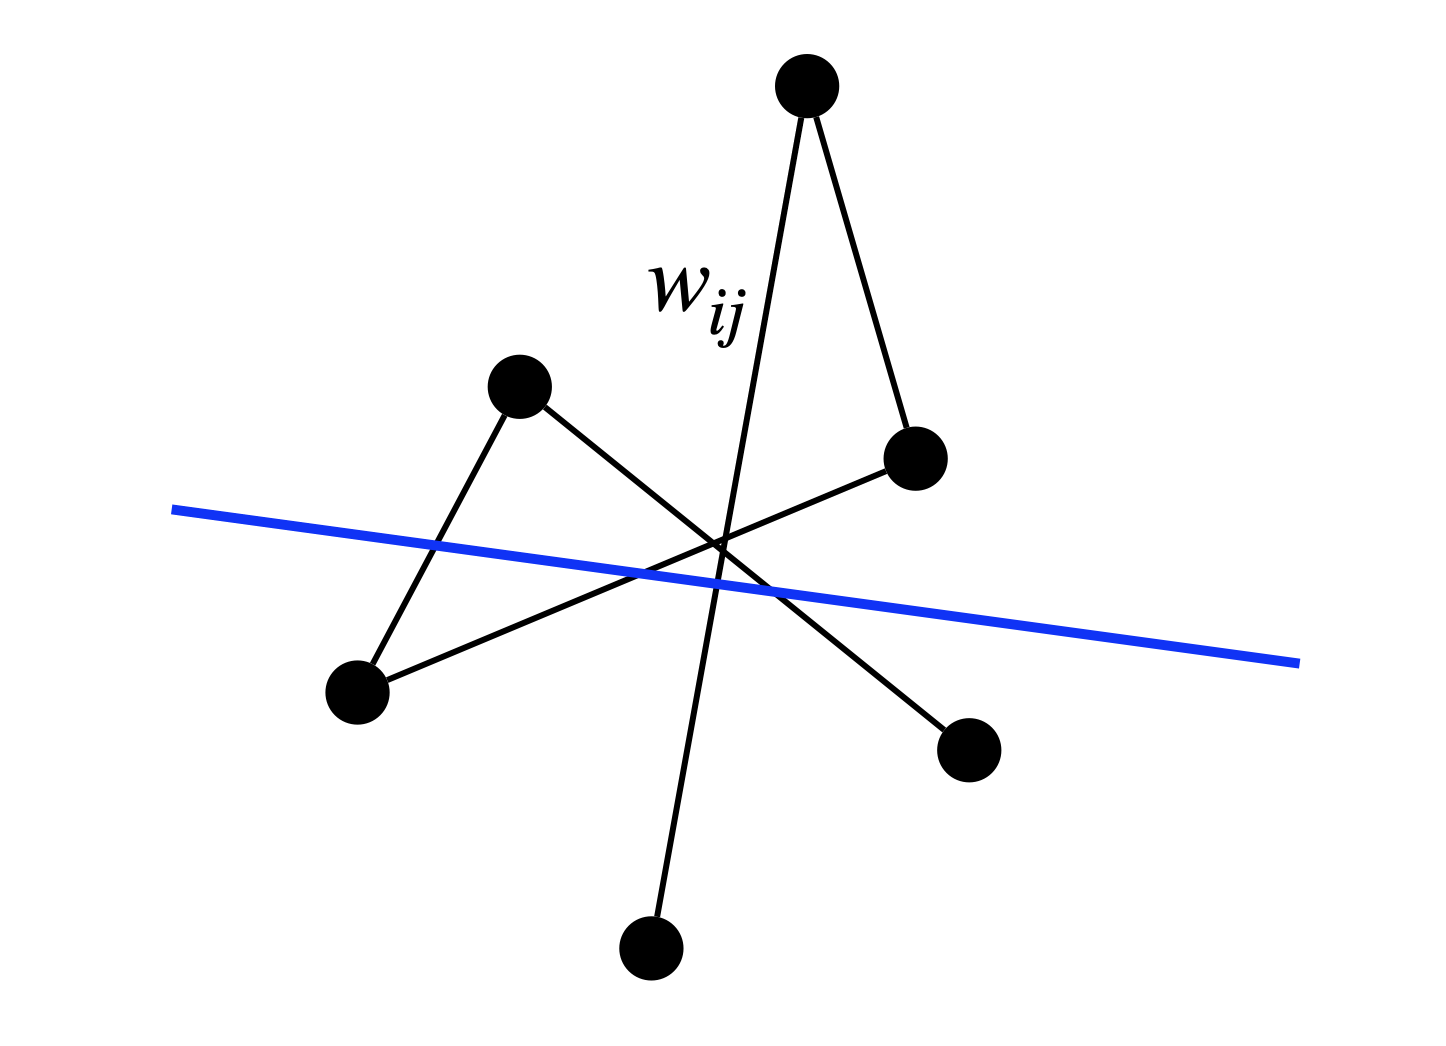
\includegraphics[width=0.6\linewidth]{images/max_cut} 

}

\caption{MAXCUT seeks to separate the node set of a graph into two disjoint groups such that the separation line cuts as many (weighted) edges as possible. For example, the blue line cuts four edges.}\label{fig:MAXCUT}
\end{figure}

Removing the constant terms in \eqref{eq:maxcut-org}, it is equivalent to the followng BQP
\begin{equation}
\min_{x_i^2 = 1}  \sum_{i,j} w_{ij} x_i x_j.
\label{eq:maxcut-bqp}
\end{equation}

\textbf{Random Rounding}. In general, solving the SDP relaxation of the MAXCUT problem will not produce a certifiably optimal solution. It is therefore interesting to ask if solving the SDP relaxation can produce provably good approximations.

Let \(X\) be the optimal solution of the SDP relaxation, and \(X = V^\top V\) be a rank-\(r\) factorization with \(V \in \mathbb{R}^{r \times n}\)
\[
V = [v_1,\dots,v_n]
\]
and each vector \(v_i \in \mathbb{R}^{r}\). We have \(X_{ij} = v_i^\top v_j\). Since \(X_{ii} = 1\), the vectors \(v_i\)'s lie on the unit sphere. Goemans and Williamson \citep{goemans95jacm-improved} proposed to obtain a feasible point to the orignal BQP by first choosing a random unit direction \(p \in \mathbb{R}^{r}\) and then assign
\[
x_i = \mathrm{sgn}(p^\top v_i), i=1,\dots,n.
\]
The expected value of this solution can be written as
\[
\mathbb{E}_p  \left\{ x^\top C x \right\}  = \sum_{i,j} C_{ij} \mathbb{E}_p  \left\{ x_i x_j \right\}  = \sum_{i,j} C_{ij} \mathbb{E}_p  \left\{ \mathrm{sgn}(p^\top x_i) \mathrm{sgn}(p^\top x_j) \right\} .
\]
This expectation can be computed using geometric intuition. Consider the plane spanned by \(v_i\) and \(v_j\) and let \(\theta_{ij}\) be the angle between them. Then, it is easy to see that the desired expectation is equal to the probability that both points are on the same side of the hyperplane, minus the probability that they are on different sides. These probabilities are \(1- \theta_{ij} / \pi\) and \(\theta_{ij} / \pi\), respectively. Therefore, the expected value of the rounded solution is
\[
\sum_{i,j} C_{ij} \left( 1- \frac{2\theta_{ij}}{\pi} \right) = \sum_{i,j} C_{ij} \left( 1- \frac{2}{\pi} \arccos (v_i^\top v_j)  \right) = \frac{2}{\pi} \sum_{i,j} C_{ij} \arcsin X_{ij},
\]
where we have used
\[
\arccos t + \arcsin t = \frac{\pi}{2}.
\]

\textbf{MAXCUT Bound}. For the MAXCUT problem, there are constant terms involved in the original cost function, which leads to the expected cut of the rounded solution to be
\[
c_{\mathrm{expected}} = \frac{1}{4} \sum_{i,j} w_{ij} \left( 1- \frac{2}{\pi} \arcsin X_{ij} \right) = \frac{1}{4} \frac{2}{\pi} \sum_{ij} w_{ij} \arccos X_{ij}.
\]
On the other hand, the optimal value of the SDP relaxation produces an upper bound on the true MAXCUT
\[
c_{\mathrm{ub}} = \frac{1}{4} \sum_{i,j} w_{ij} (1 - X_{ij}).
\]
We have
\[
c_{\mathrm{expected}} \leq c_{\mathrm{MAXCUT}} \leq c_{\mathrm{ub}}.
\]
We want to find the maximum possible \(\alpha\) such that
\[
\alpha c_{\mathrm{ub}} \leq c_{\mathrm{expected}} \leq c_{\mathrm{MAXCUT}} \leq c_{\mathrm{ub}},
\]
so that \(\alpha\) acts to be the best approximation ratio. To find such \(\alpha\), we need to find the maximum \(\alpha\) such that
\[
\alpha (1 - t) \leq \frac{2}{\pi} \arccos(t), \forall t \in [-1,1].
\]
The best possible \(\alpha\) is \(0.878\), see Fig. \ref{fig:MAXCUTAlpha}.

\begin{figure}

{\centering 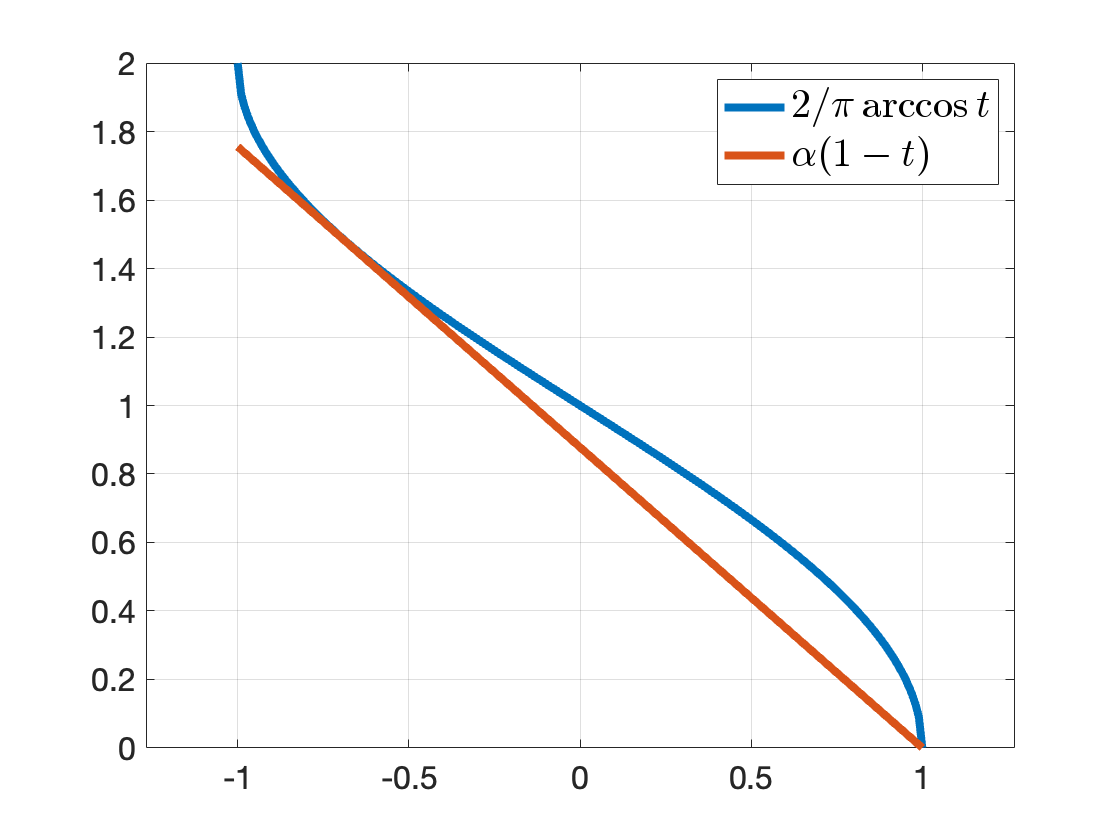
\includegraphics[width=0.6\linewidth]{images/maxcut_alpha} 

}

\caption{Best approximation ratio.}\label{fig:MAXCUTAlpha}
\end{figure}

\hypertarget{certifiably-optimal-rotation-averaging}{%
\section{Certifiably Optimal Rotation Averaging}\label{certifiably-optimal-rotation-averaging}}

Consider a graph \(\mathcal{G}= (\mathcal{V},\mathcal{E})\) with node set \(\mathcal{V}= [N]\) and edge set \(\mathcal{E}= \{(i,j) \mid i,j \in \mathcal{V}\}\). Each node \(i\) is associated with an unknown rotation matrix \(R_i \in \mathrm{SO}(3)\), and each edge is associated with a relative rotation
\begin{equation}
\tilde{R}_{ij} = R_i^\top R_j \cdot R_{\epsilon},
\label{eq:rotation-averaging-gen-model}
\end{equation}
that measures the relative rotation between \(R_i\) and \(R_j\), up to some small noise corruption \(R_{\epsilon} \in \mathrm{SO}(3)\). See Fig. \ref{fig:RotationAveraging}.

The goal of (multiple) rotation averaging is to estimate the absolute rotations \(\{R_i \}_{i=1}^N\) given the noisy relative rotation measurements on the edges \(\{\tilde{R}_{ij} \}_{(i,j) \in \mathcal{E}}\). This problem is also known as rotation synchronization and it finds applications in computer vision \citep{eriksson18cvpr-rotation}, robotics \citep{rosen19ijrr-sesync}, and medical imaging \citep{wang13ima-exact}.

\begin{figure}

{\centering 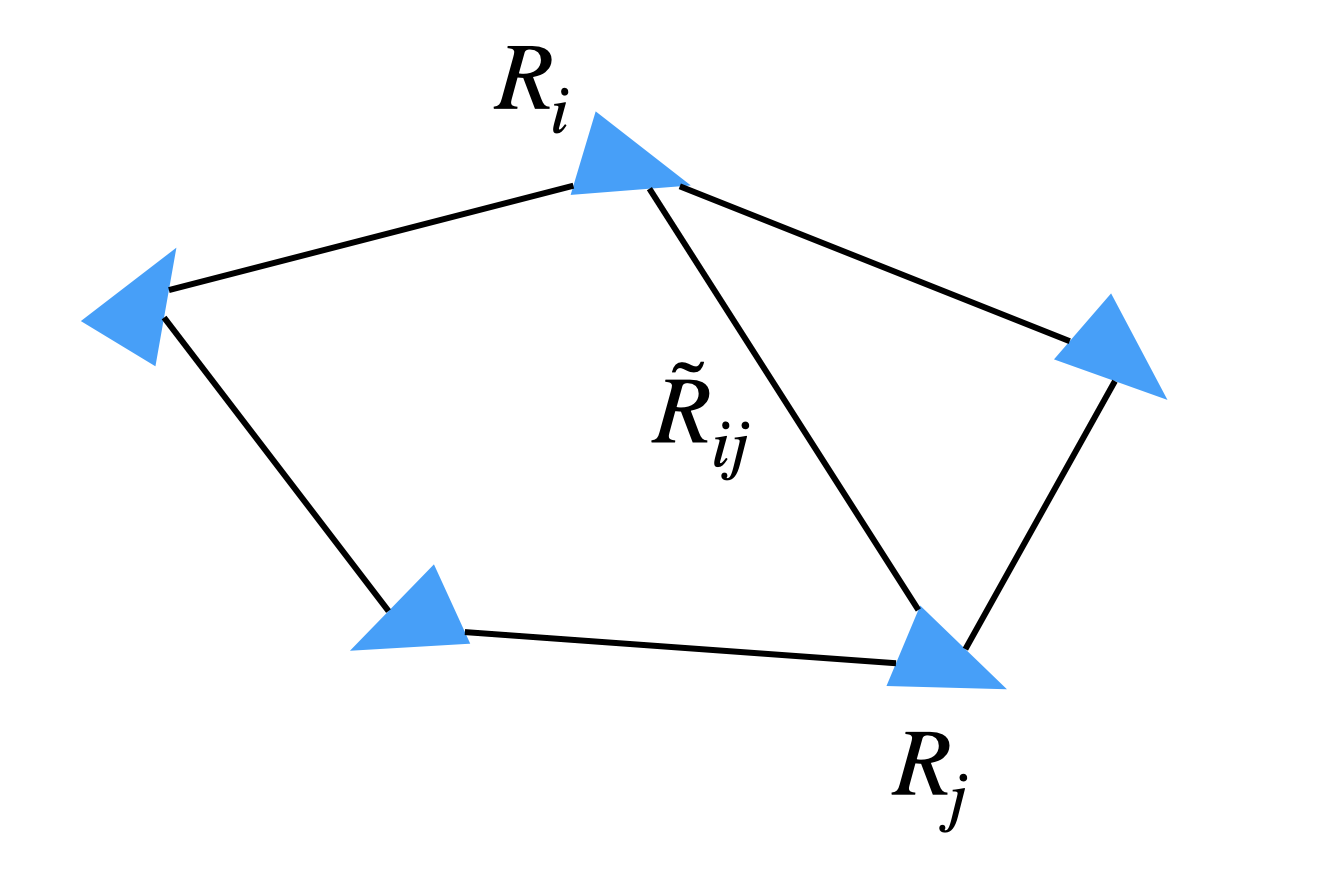
\includegraphics[width=0.6\linewidth]{images/rotation_avg} 

}

\caption{Rotation Averaging.}\label{fig:RotationAveraging}
\end{figure}

To synchronize the absolute rotations from relative measurements, it is common practice to formulate the following optimization problem
\begin{equation}
\min_{R_i \in \mathrm{SO}(3), i\in \mathcal{V}} \sum_{(i,j) \in \mathcal{E}} \Vert \tilde{R}_{ij} - R_i^\top R_j \Vert_\mathrm{F}^2,
\label{eq:rotation-averaging}
\end{equation}
to seek the best absolute rotations that fit the relative measurements according to the generative model \eqref{eq:rotation-averaging-gen-model}. It can be shown that when the noise \(R_\epsilon\) satisfies a Langevin distribution, then problem \eqref{eq:rotation-averaging} returns the maximum likelihood estimator. Even when the noise distribution is not Langevin, problem \eqref{eq:rotation-averaging} often produces accurate estimates.

\textbf{QCQP Formulation}. We will first simplify problem \eqref{eq:rotation-averaging} as a QCQP. Note that the objective is equivalent to
\[
\sum_{(i,j) \in \mathcal{E}} \mathrm{tr}\left( (\tilde{R}_{ij} - R_i^\top R_j)^\top(\tilde{R}_{ij} - R_i^\top R_j) \right) = \sum_{(i,j) \in \mathcal{E}} \mathrm{tr}\left( 2 \mathrm{I}_3 - 2 \tilde{R}_{ij}^\top R_i^\top R_j \right).
\]
Therefore, problem \eqref{eq:rotation-averaging} is equivalent to
\begin{equation}
\min_{R_i \in \mathrm{SO}(3), i\in\mathcal{V}} -2\sum_{(i,j)\in\mathcal{E}} \mathrm{tr}(\tilde{R}_{ij}^\top R_i^\top R_j).
\label{eq:rotation-averaging-qcqp}
\end{equation}
This is a QCQP because the objective is quadratic, and \(\mathrm{SO}(3)\) can be described by quadratic equality constraints.

\textbf{Matrix Formulation}. Let
\[
R = \begin{bmatrix} 
R_1^\top\\
\vdots \\
R_N^\top
\end{bmatrix} \in \mathrm{SO}(3)^N,\quad 
RR^\top= \begin{bmatrix}
R_1^\top R_1 & R_1^\top R_2 & \cdots & R_1^\top R_N \\
R_2^\top R_1 & R_2^\top R_2 & \cdots & R_2^\top R_N \\
\vdots & \vdots & \ddots & \vdots \\
R_N^\top R_1 & R_N^\top R_2 & \cdots & R_N^\top R_N
\end{bmatrix} \in \mathbb{S}^{3N}_{+}
\]
and
\begin{equation}
\tilde{R}= \begin{bmatrix}
0 & \tilde{R}_{12} & \cdots & \tilde{R}_{1N} \\
\tilde{R}_{12}^\top& 0 & \cdots & \tilde{R}_{2N}\\
\vdots & \vdots & \ddots & \vdots \\
\tilde{R}_{1N}^\top& \tilde{R}_{2N}^\top& \cdots & 0
\end{bmatrix} \in \mathbb{S}^{3N}
\label{eq:rotation-averaging-tldR}
\end{equation}
Then problem \eqref{eq:rotation-averaging-qcqp} can be compactly written as
\begin{equation}
\min_{R \in \mathrm{SO}(3)^N} - \langle \tilde{R}, RR^\top \rangle
\label{eq:rotation-averaging-matrix}
\end{equation}

\textbf{Semidefinite Relaxation}. Problem \eqref{eq:rotation-averaging-matrix} is nonconvex, so we apply semidefinite relaxation. Observe that, because \(R_i \in \mathrm{SO}(3)\), we have
\[
R_i^\top R_i = \mathrm{I}_3, \forall i=1,\dots,N.
\]
Therefore, the diagonal blocks of \(RR^\top\) are all \(3\times 3\) identity matrices. We have also that \(RR^\top\succeq 0\) by construction. Therefore, the following SDP is a convex relaxation of problem \eqref{eq:rotation-averaging-matrix}
\begin{equation}
\begin{split}
\min_{X \in \mathbb{S}^{3N}} & \quad - \langle \tilde{R}, RR^\top \rangle \\
\mathrm{s.t.}& \quad X \succeq 0 \\
& \quad [X]_{ii} = \mathrm{I}_3, \quad i=1,\dots,N
\end{split}
\label{eq:rotation-averaging-sdp-relax}
\end{equation}
where the last constraint in \eqref{eq:rotation-averaging-sdp-relax} enforces all diagonal blocks to be identity matrices.

How powerful is this SDP relaxation? You may think that it will be quite loose (and hence not very useful) because we have dropped many nonconvex constraints from the original QCQP to the convex SDP (e.g., \(\mathrm{rank}(X) = 3\), \(R_i \in \mathrm{SO}(3)\) but we only used \(R_i \in \mathrm{O}(3)\)), but empirically it is almost always exact.

\begin{example}[Rotation Averaging]
\protect\hypertarget{exm:RotationAveraging}{}\label{exm:RotationAveraging}I will generate a fully connected graph \(\mathcal{G}\) with \(N\) nodes.

\begin{itemize}
\item
  For each node \(i\), I associate a random 3D rotation matrix \(R_i\). For the first node, I always let \(R_1 = \mathrm{I}_3\).
\item
  For each edge \((i,j)\), I generate a noisy measurement
  \[
  \tilde{R}_{ij} = R_i^\top R_j \cdot R_\epsilon,
  \]
  where \(R_\epsilon\) is a rotation matrix with a random rotation axis and a rotation angle uniformally distributed between \(0\) and \(\beta\) degrees.
\end{itemize}

After this graph is generated, I form the \(\tilde{R}\) matrix in \eqref{eq:rotation-averaging-tldR} and solve the SDP \eqref{eq:rotation-averaging-sdp-relax}. This can be easily programmed in Matlab:

\begin{Shaded}
\begin{Highlighting}[]
\VariableTok{X} \OperatorTok{=} \VariableTok{sdpvar}\NormalTok{(}\FloatTok{3}\OperatorTok{*}\VariableTok{n}\OperatorTok{,}\FloatTok{3}\OperatorTok{*}\VariableTok{n}\NormalTok{)}\OperatorTok{;}
\VariableTok{F} \OperatorTok{=}\NormalTok{ [}\VariableTok{X} \OperatorTok{\textgreater{}=} \FloatTok{0}\NormalTok{]}\OperatorTok{;}
\KeywordTok{for} \VariableTok{i} \OperatorTok{=} \FloatTok{1}\OperatorTok{:}\VariableTok{n}
    \VariableTok{F} \OperatorTok{=}\NormalTok{ [}\VariableTok{F}\OperatorTok{,}
        \VariableTok{X}\NormalTok{(}\VariableTok{blkIndices}\NormalTok{(}\VariableTok{i}\OperatorTok{,}\FloatTok{3}\NormalTok{)}\OperatorTok{,}\VariableTok{blkIndices}\NormalTok{(}\VariableTok{i}\OperatorTok{,}\FloatTok{3}\NormalTok{)) }\OperatorTok{==} \VariableTok{eye}\NormalTok{(}\FloatTok{3}\NormalTok{)]}\OperatorTok{;}
\KeywordTok{end}
\VariableTok{obj} \OperatorTok{=} \VariableTok{trace}\NormalTok{(}\OperatorTok{{-}}\VariableTok{Rtld}\OperatorTok{*}\VariableTok{X}\NormalTok{)}\OperatorTok{;}
\VariableTok{optimize}\NormalTok{(}\VariableTok{F}\OperatorTok{,}\VariableTok{obj}\NormalTok{)}\OperatorTok{;}
\VariableTok{Xval} \OperatorTok{=} \VariableTok{value}\NormalTok{(}\VariableTok{X}\NormalTok{)}\OperatorTok{;}
\VariableTok{f\_sdp} \OperatorTok{=} \VariableTok{value}\NormalTok{(}\VariableTok{obj}\NormalTok{)}\OperatorTok{;}
\end{Highlighting}
\end{Shaded}

Note that \texttt{f\_sdp} will be a lower bound.

Let \(X_\star\) be the optimal solution of the SDP. We know that, if the SDP relaxation is tight, then \(X_\star\) will look like \(RR^\top\). Because \(R_1 = \mathrm{I}_3\), we can directly read off the optimal rotation estimations from the first row of blocks. However, if the relaxation is not tight, the blocks there will not be valid rotation matrices, and we can perform a projection onto \(\mathrm{SO}(3)\). Using the estimated rotations, I can compute \texttt{f\_est}, which is an upper bound to the true global optimum.

\begin{Shaded}
\begin{Highlighting}[]
\VariableTok{R\_est} \OperatorTok{=}\NormalTok{ []}\OperatorTok{;}
\VariableTok{R\_errs} \OperatorTok{=}\NormalTok{ []}\OperatorTok{;}
\KeywordTok{for} \VariableTok{i} \OperatorTok{=} \FloatTok{1}\OperatorTok{:}\VariableTok{n}
    \KeywordTok{if} \VariableTok{i} \OperatorTok{==} \FloatTok{1}
        \VariableTok{Ri} \OperatorTok{=} \VariableTok{eye}\NormalTok{(}\FloatTok{3}\NormalTok{)}\OperatorTok{;}
    \KeywordTok{else}
        \VariableTok{Ri} \OperatorTok{=} \VariableTok{project2SO3}\NormalTok{(}\VariableTok{Xval}\NormalTok{(}\FloatTok{1}\OperatorTok{:}\FloatTok{3}\OperatorTok{,}\VariableTok{blkIndices}\NormalTok{(}\VariableTok{i}\OperatorTok{,}\FloatTok{3}\NormalTok{)))}\OperatorTok{;}
    \KeywordTok{end}
    \VariableTok{R\_errs} \OperatorTok{=}\NormalTok{ [}\VariableTok{R\_errs}\OperatorTok{,} \VariableTok{getAngularError}\NormalTok{(}\VariableTok{Ri}\OperatorTok{,} \VariableTok{R\_gt}\NormalTok{(}\VariableTok{blkIndices}\NormalTok{(}\VariableTok{i}\OperatorTok{,}\FloatTok{3}\NormalTok{)}\OperatorTok{,:}\NormalTok{))]}\OperatorTok{;}
    \VariableTok{R\_est} \OperatorTok{=}\NormalTok{ [}\VariableTok{R\_est}\OperatorTok{,} \VariableTok{Ri}\NormalTok{]}\OperatorTok{;}
\KeywordTok{end}
\VariableTok{X\_est} \OperatorTok{=} \VariableTok{R\_est}\OperatorTok{\textquotesingle{}*}\VariableTok{R\_est}\OperatorTok{;}
\VariableTok{f\_est} \OperatorTok{=} \VariableTok{trace}\NormalTok{(}\OperatorTok{{-}}\VariableTok{Rtld}\OperatorTok{*}\VariableTok{X\_est}\NormalTok{)}\OperatorTok{;}
\end{Highlighting}
\end{Shaded}

With \texttt{f\_est} and \texttt{f\_sdp}, an upper bound and a lower bound, I can compute the relative suboptimality gap \(\eta\). If \(\eta = 0\), then it certifies global optimality.

How does this work?

For \(N=30\) and \(\beta = 10\) (small noise), I got \(\eta = 6.26\times 10^{-13}\). Fig. \ref{fig:MVA-rot-err-30-10} plots the rotation estimation errors at each node compared to the groundtruth rotations.

\begin{figure}

{\centering 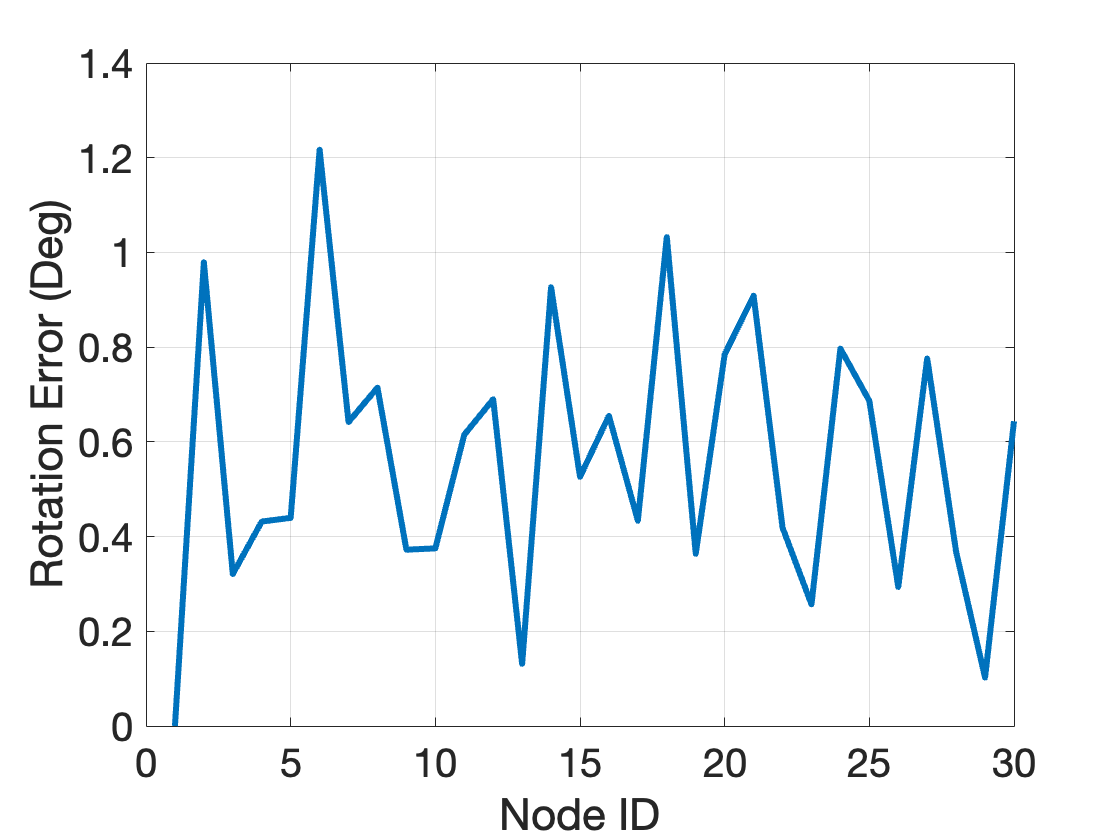
\includegraphics[width=0.6\linewidth]{images/mva_rot_err_30_10} 

}

\caption{Rotation estimation errors, 30 nodes, noise bound 10 degrees.}\label{fig:MVA-rot-err-30-10}
\end{figure}

What if I increase the noise bound to \(\beta = 60\)? It turns out the relaxation is still exact with \(\eta = 6.84 \times 10^{-10}\)! Fig. \ref{fig:MVA-rot-err-30-60} plots the rotation estimation errors at each node compared to the groundtruth rotations.

\begin{figure}

{\centering 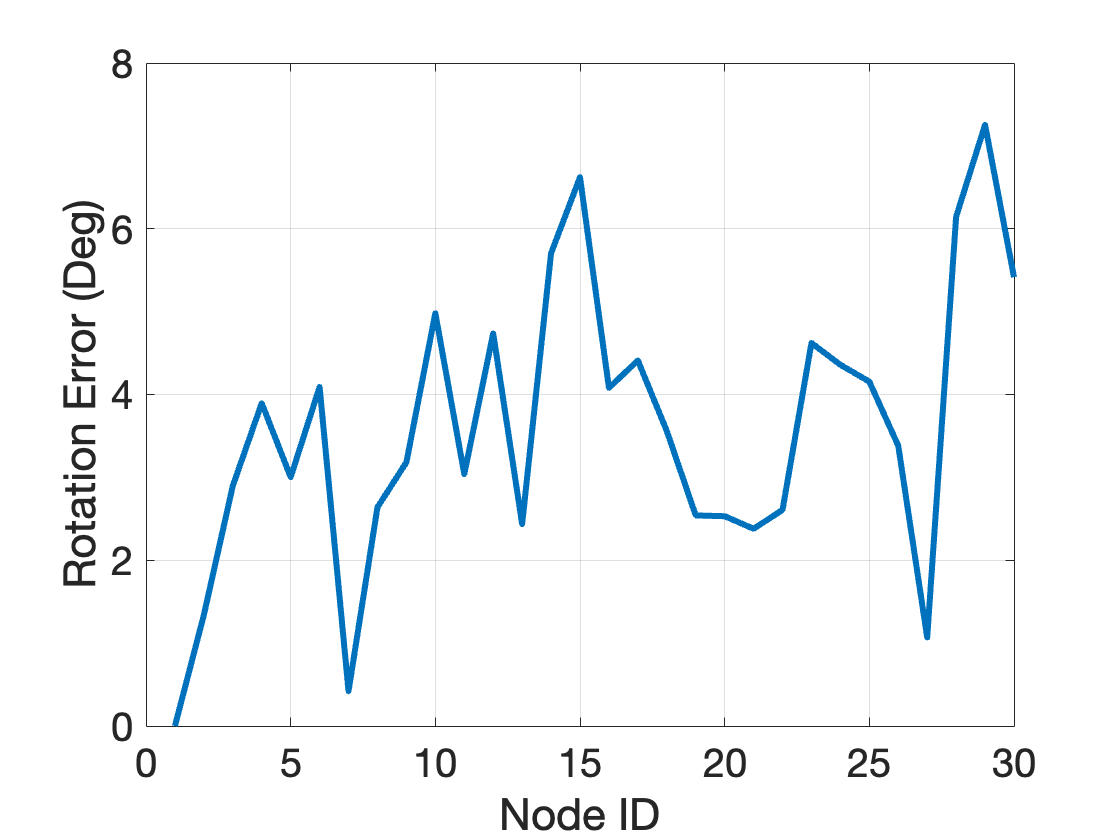
\includegraphics[width=0.6\linewidth]{images/mva_rot_err_30_60} 

}

\caption{Rotation estimation errors, 30 nodes, noise bound 60 degrees.}\label{fig:MVA-rot-err-30-60}
\end{figure}

What if I set \(\beta = 120\)? The relaxation still remains exact with \(\eta = 9.5 \times 10^{-10}\). Fig. \ref{fig:MVA-rot-err-30-120} plots the rotation estimation errors at each node compared to the groundtruth rotations. Observe that even when the rotation estimates have large errors, they are still the certifiably optimal estimates.

\begin{figure}

{\centering 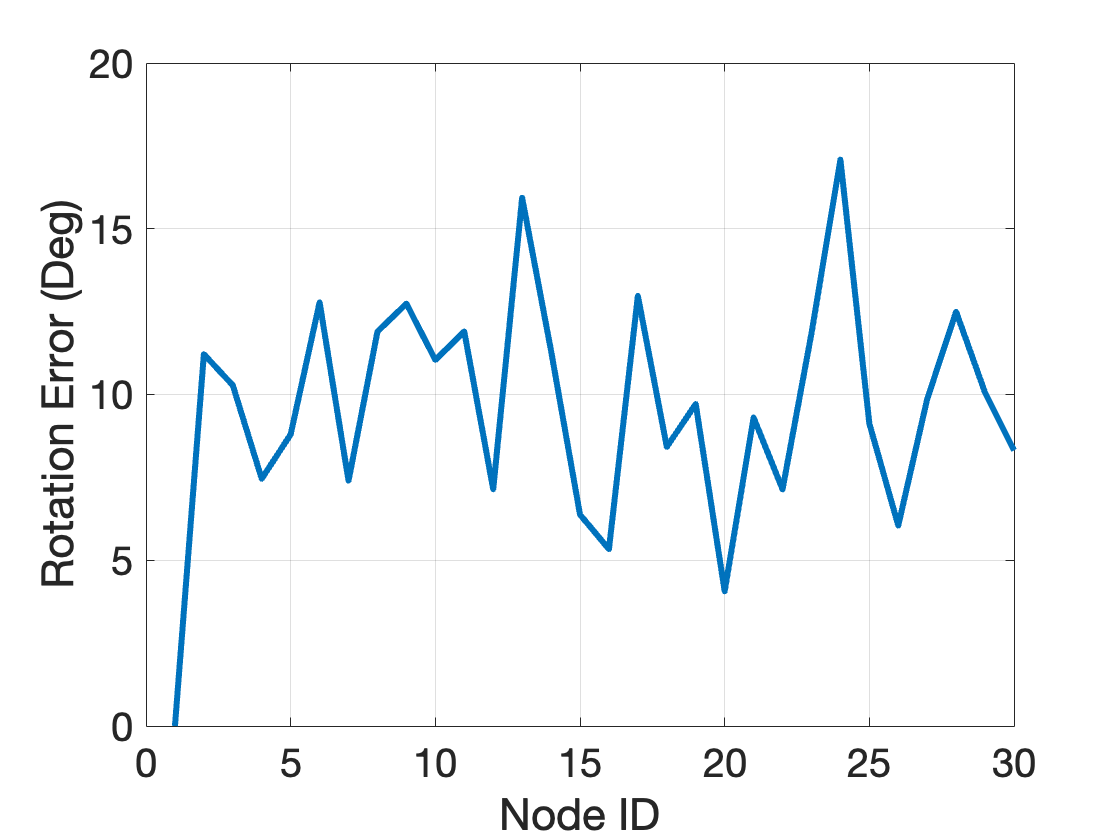
\includegraphics[width=0.6\linewidth]{images/mva_rot_err_30_120} 

}

\caption{Rotation estimation errors, 30 nodes, noise bound 120 degrees.}\label{fig:MVA-rot-err-30-120}
\end{figure}

Play with the \href{https://github.com/ComputationalRobotics/Semidefinite-Examples/blob/main/rotation_averaging/example.m}{code} yourself to appreciate the power of this simple SDP relaxation. You can, for example, increase the number of nodes \(N\). What if you make the graph sparse (e.g., fewer edges but still a connected graph)?
\end{example}

\hypertarget{dual-optimality-certifier}{%
\subsection{Dual Optimality Certifier}\label{dual-optimality-certifier}}

\hypertarget{stretch-to-high-degree-polynomial-optimization}{%
\section{Stretch to High-Degree Polynomial Optimization}\label{stretch-to-high-degree-polynomial-optimization}}

We have seen that Shor's semidefinite relaxation for QCQPs can be derived both using Lagrangian duality, or simply by dropping a rank constraint, both of which are straightforward to understand. When applied to the MAXCUT problem, it produces a provably good approximation ratio. When applied to the rotation averaging problem, it directly gives us the optimal solution without any approximation, and the optimality comes with a certificate.

However, not every optimization problem is a QCQP, right? Is it possible to generalize Shor's semidefinite relaxation to higher-degree polynomial optimization problems? As we will see in the next Chapters, the moment and sums-of-squares (SOS) hierarchy delivers the perfect and principled generalization.

Before going to the moment-SOS hierarchy, let me give you an example of a quartic (degree-4) optimization problem, for which we can still use Shor's relaxation, albeit with some (in my opinion, not so elegant) mathematical massage. This example in fact is from a recent paper in computer vision \citep{briales18cvpr-certifiably}.

\textbf{Two-view Geometry}. Consider the problem of estimating the motion of a camera from two views illustrated in Fig. \ref{fig:two-view}. Let \(C_1\) and \(C_2\) be two cameras (or the same camera but in two different positions) observing the same 3D point \(p \in \mathbb{R}^{3}\). The 3D point will be observed by \(C_1\) and \(C_2\) via its 2D projections on the image plane, respectively. Let \(f_1 \in \mathbb{R}^{3}\) and \(f_2 \in \mathbb{R}^{3}\) be the unit-length bearing vector that emanates from the camera centers to the 2D projections in two cameras, respectively. Our goal is to estimate the relative rotation and translation between the two cameras \(C_1\) and \(C_2\), denoted by \(R \in \mathrm{SO}(3)\) and \(t \in \mathbb{R}^{3}\). The pair of bearing vectors \((f_1,f_2)\) is typically known as a \textbf{correspondence}, or a \textbf{match} in computer vision.

\begin{figure}

{\centering 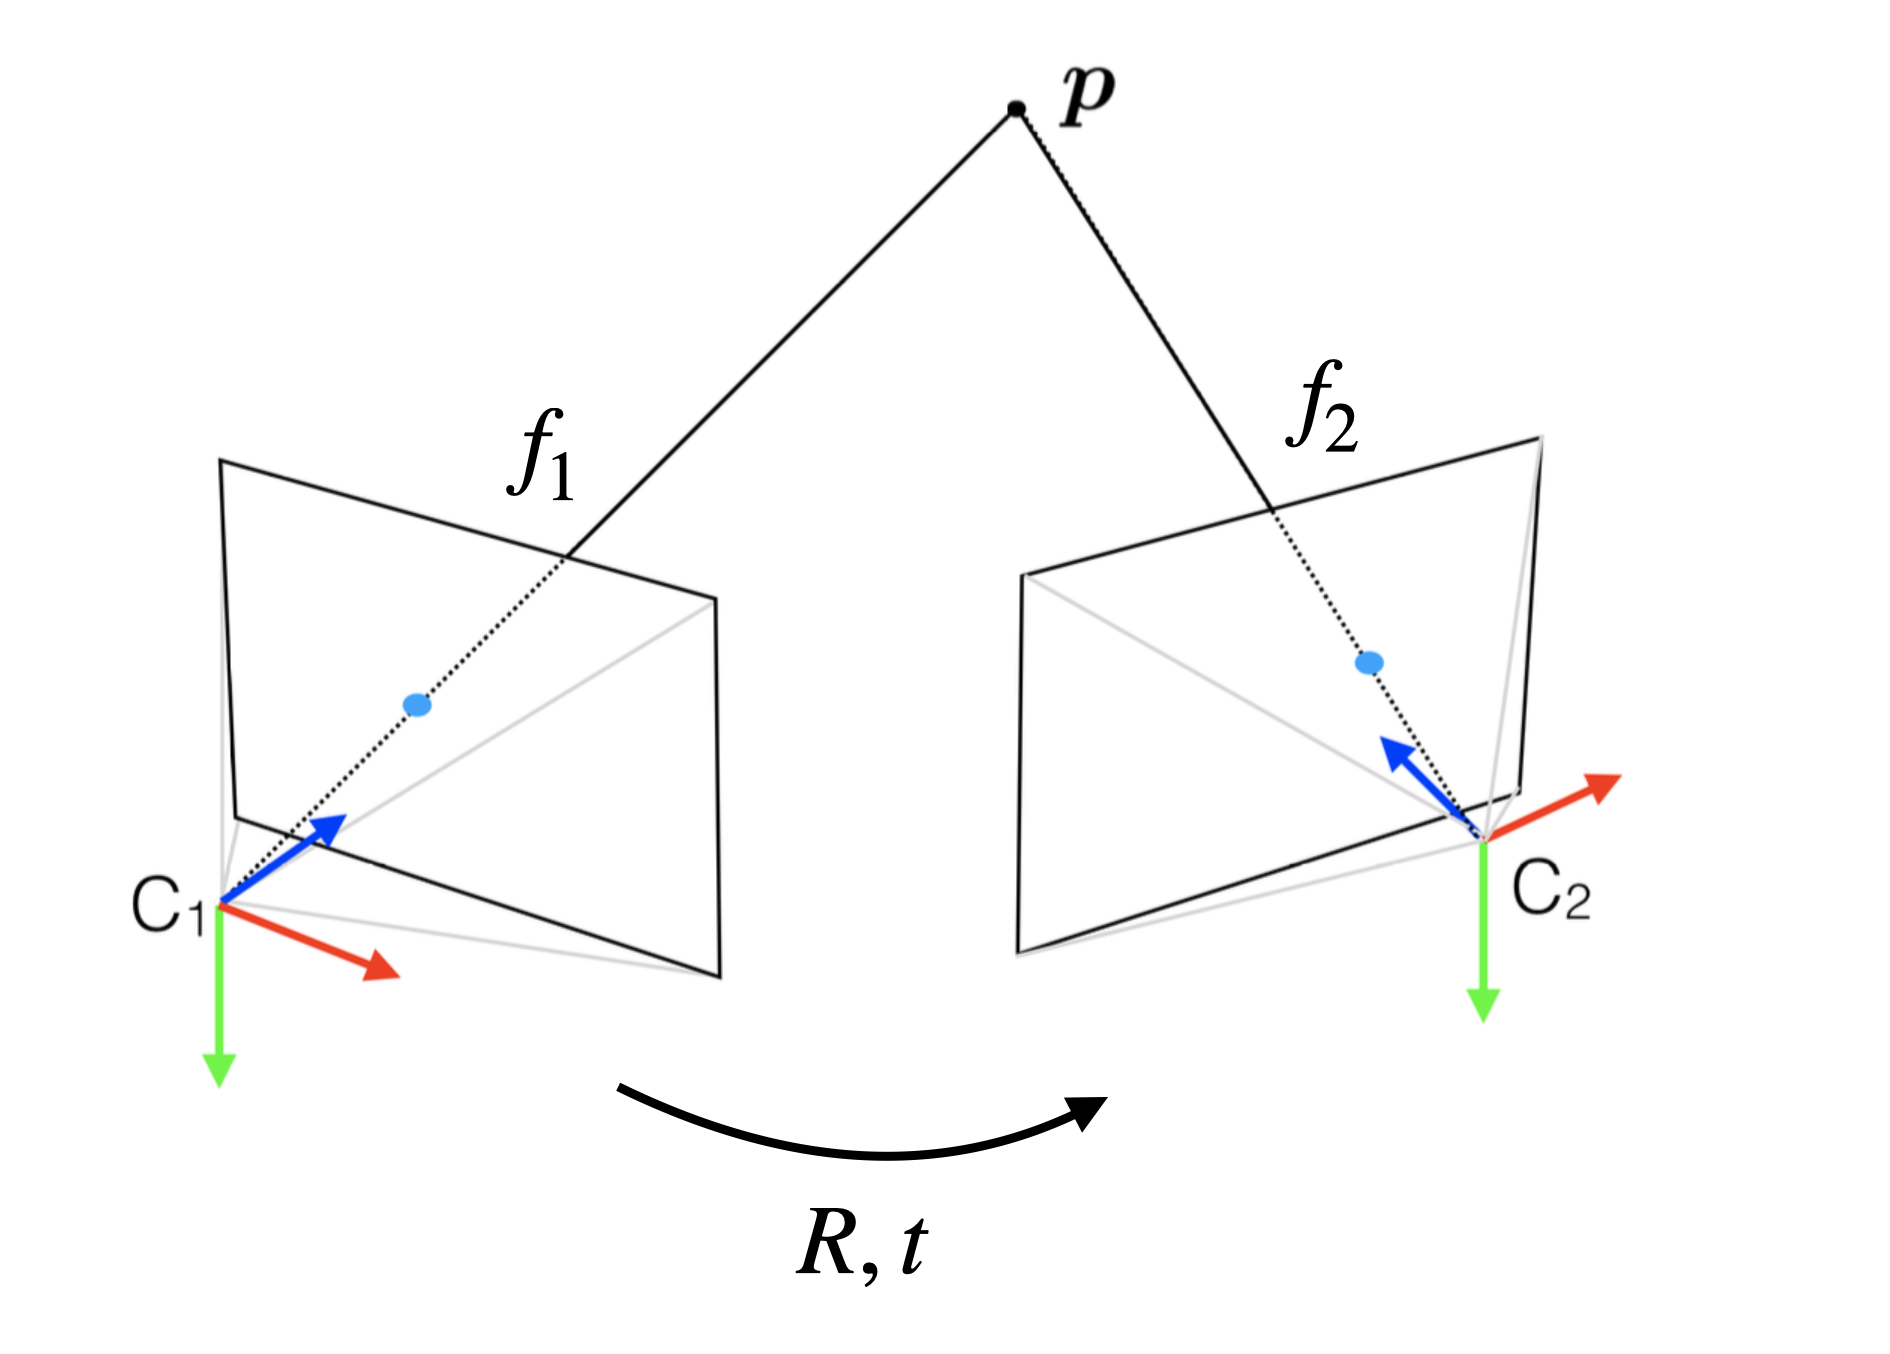
\includegraphics[width=0.6\linewidth]{images/two_view} 

}

\caption{Two-view Geometry.}\label{fig:two-view}
\end{figure}

It turns out only having one correspondence is insufficient to recover \((R,t)\), and we need at least \(5\) such correspondences \citep{nister04pami-efficient}. See Fig. \ref{fig:two-view-example} for an example I adapted from \href{https://www.mathworks.com/help/vision/ref/estimateessentialmatrix.html}{Mathworks}.

\begin{figure}

{\centering 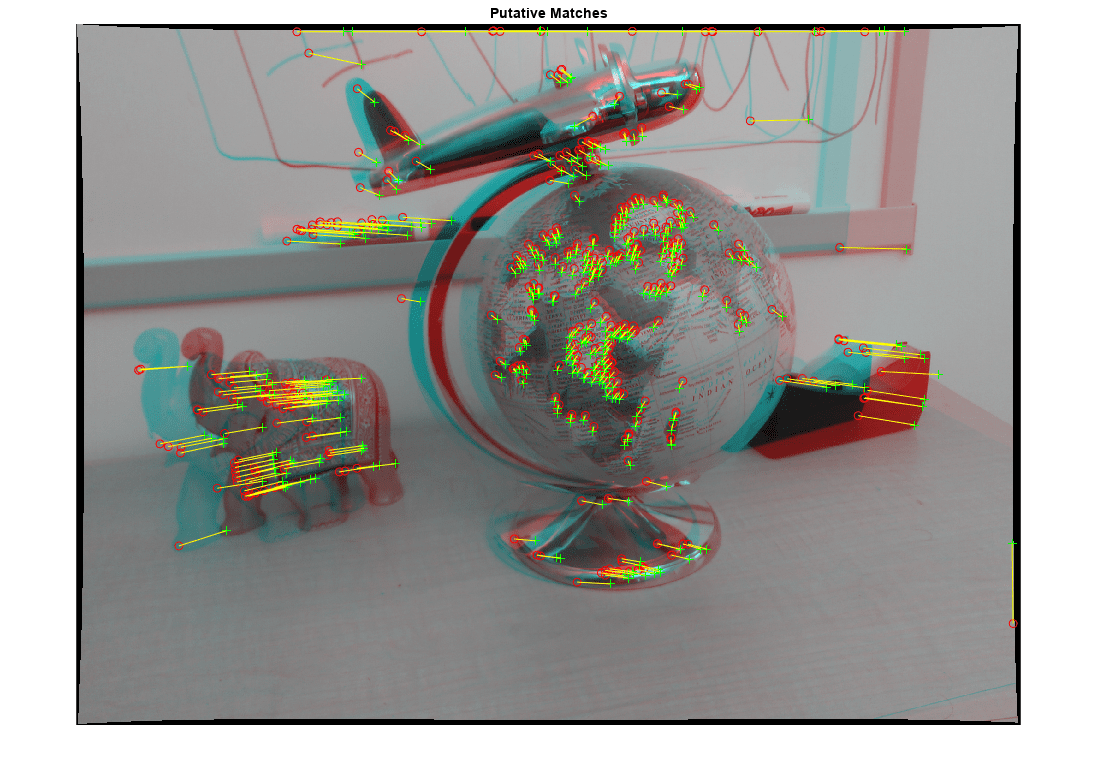
\includegraphics[width=0.8\linewidth]{images/two_view_example_matlab} 

}

\caption{A real two-view motion estimation example. Copyright: Mathworks.}\label{fig:two-view-example}
\end{figure}

Consequently, to formally state our problem, we are given a set of \(N\) correspondences (these correspondences are typically detected by neural networks today \citep{wang20eccv-caps})
\[
\{f_{1,i},f_{2,i} \}_{i=1}^N
\]
between two images taken by two cameras, and our goal is to estimate the relative motion \((R,t)\).

\textbf{Epipolar Constraint}. When the correspondences are noise-free, it is known that they must satisfy the following epipolar constraint \citep{hartley03book-multiple}
\begin{equation}
f_{2,i}^\top[t]_{\times} R f_{1,i} = 0, \quad \forall i=1,\dots,N,
\label{eq:epipolar-constraint}
\end{equation}
where
\[
[t]_{\times} := \begin{bmatrix} 0 & - t_3 & t_2 \\
t_3 & 0 & - t_1 \\
- t_2 & t_1 & 0 \end{bmatrix}
\]
is a linear map such that \(t \times v = [t]_{\times} v\) for any \(v \in \mathbb{R}^{3}\) and \(\times\) denotes cross product in 3D.

\textbf{Nonlinear Least Squares}. Since the correspondences are detected by neural networks, they will be noisy and the epipolar constraint \eqref{eq:epipolar-constraint} will not be perfectly satisfied. Therefore, we formulate the following optimization problem to seek the best estimate that minimize the sum of the squared violations of \eqref{eq:epipolar-constraint}
\begin{equation}
\min_{R \in \mathrm{SO}(3), t \in \mathcal{S}^{2}} \sum_{i=1}^N (f_{2,i}^\top[t]_{\times} R f_{1,i})^2
\label{eq:two-view-estimation-problem}
\end{equation}
Note that I have asked \(t \in \mathcal{S}^{2}\) to lie on the unit sphere, why?

Problem \eqref{eq:two-view-estimation-problem} is not a QCQP anymore, because its objective is a degree-4 polynomial. However, all the constraints of \eqref{eq:two-view-estimation-problem} are quadratic equalities and inequalities. To see this, note that \(t \in \mathcal{S}^{2}\) can be written as
\begin{equation}
1 - t^\top t = 0,
\label{eq:two-view-t-con}
\end{equation}
which is a quadratic polynomial equality.
The constraint \(R \in \mathrm{SO}(3)\) can also be written as quadratic equalities. Let
\[
R = [c_1, c_2, c_3]
\]
where \(c_i\) is the \(i\)-the column. Then \(R\in \mathrm{SO}(3)\) is equivalent to
\begin{equation}
\begin{split}
c_i^\top c_i - 1= 0, & \quad i=1,2,3 \\
c_i^\top c_j = 0, & \quad (i,j) \in \{ (1,2),(2,3),(3,1) \} \\
c_i \times c_j = c_k,& \quad (i,j,k) \in \{ (1,2,3),(2,3,1),(3,1,2) \}. 
\end{split}
\label{eq:two-view-R-con}
\end{equation}
all of which are quadratic polynomial equalities.

Let \(r = \mathrm{vec}(R)\), \(x = [r^\top, t^\top]^\top\in \mathbb{R}^{12}\), we will collectively call all the constraints in \eqref{eq:two-view-t-con} and \eqref{eq:two-view-R-con} as
\[
h_k(x) = 0, k=1,\dots,l, 
\]
with \(l=16\).

\textbf{Semidefinite Relaxation}. Clearly, we cannot directly apply Shor's semidefinite relaxation, because \(X = xx^\top\) only contains monomials in \(x\) of degree up to \(2\), but our objective function is degree \(4\) -- this matrix variable is not powerful enough.

To fix this issue, a natural idea is to create a larger matrix variable
\begin{equation}
\hspace{-16mm}
v = \begin{bmatrix} 
1 \\ r \\ t \\ t_1 r \\ t_2 r \\ t_3 r \end{bmatrix} \in \mathbb{R}^{40}, \quad X = vv^\top= \begin{bmatrix} 1 & * & * & * & * & * \\
r & rr^\top& * & * & * & * \\
t & tr^\top& tt^\top& * & * & * \\
t_1 r & t_1 rr^\top& t_1 r t^\top& t_1^2 rr^\top& * & * \\
t_2 r & t_2 rr^\top& t_2 r t^\top& t_1 t_2 rr^\top& t_2^2 rr^\top& * \\
t_3 r & t_3 rr^\top& t_3 r t^\top& t_3 t_1 rr^\top& t_3 t_2 rr^\top& t_3^2 rr^\top\end{bmatrix} \in \mathbb{S}^{40}_{+}
\label{eq:two-view-larger-X}
\end{equation}
Note that now \(X\) has degree-4 monomials, which allows me to write the objective of the original problem \eqref{eq:two-view-estimation-problem} as
\[
\langle C, X \rangle
\]
with a suitable constant matrix \(C \in \mathbb{S}^{40}\).

I can also write all the original constraints \(h_k(x) = 0,k=1,\dots,l\) as
\[
\langle A_k, X \rangle = 0, k=1,\dots,l,
\]
plus an additional constraint
\[
\langle A_0, X \rangle = 1, 
\]
where \(A_0\) is all zero except its top-left entry is equal to 1.

This seems to be all we need for Shor's relaxation, will this work?

\textbf{``Redundant'' Constraints}. In the original paper \citep{briales18cvpr-certifiably}, the authors found that we are missing some important constraints that we can add to the convex SDP. For example, in the matrix \(X\), we have
\[
t_1^2 rr^\top+ t_2^2 rr^\top+ t_3^2 rr^\top= (t_1^2 + t_2^2 + t_3^2) rr^\top= rr^\top,
\]
which gives us additional linear constraints on the entries of \(X\) (for free)! Essentially, these constraints are generated by multiplying the original constraints \(h_k(x)\) by suitable monomials:
\[
h_k(x) = 0 \Rightarrow h_k(x) \cdot \lambda(x) = 0,
\]
where \(\lambda(x)\) is a monomial such that all the monomials of \(h_k(x) \cdot \lambda(x)\) appear in the big matrix \(X\) (so that the resulting equality constraint can still be written as a linear equality on \(X\)). The authors of \citep{briales18cvpr-certifiably} enumerated all such constraints (by hand) and added them to the SDP relaxation, which led to the relaxation going from loose to tight/exact.

\citep{briales18cvpr-certifiably} called these constraints ``redundant'', are they? We will revisit this after we study the moment-SOS hierarchy!

  \bibliography{book.bib}

\end{document}
